\documentclass[letterpaper,tocnosub,noragright,centerchapter,12pt,edeposit]{uiucecethesis09}

\makeatletter

\usepackage{amsmath}
\usepackage{amsthm}
\usepackage{amssymb}
\usepackage{bbm}
\usepackage{bm}
\usepackage{calc}
\usepackage[justification=raggedright]{caption}
\usepackage{graphicx}
\usepackage{mathrsfs}
\usepackage{natbib}
\usepackage{psfrag}
\usepackage[overload]{textcase}
%% hyperref manual advises loading this package last
\usepackage{hyperref}
\hypersetup{colorlinks=true,linkcolor=blue,citecolor=blue,breaklinks=true}

\phdthesis

\title{Stochastic Averaging for Mechanical Systems}
\author{Kristjan Onu}
\department{Mechanical Science \& Engineering}
\degreeyear{2010}

\advisor{Professor N. Sri Namachchivaya}

\committee{Professor N. Sri Namachchivaya, Director of Dissertation Research\\
Professor Matthew West, Chair\\
Professor R. Lee DeVille\\
Professor Martin Ostoja-Starzewski}

\newcommand{\Aave}{\operatorname{\mathbf A}}
\newcommand{\Aa}{\mathfrak a}
\newcommand{\prob}{\mathbf P}
\newcommand{\Expectation}{\operatorname{\mathbf E}}
\newcommand{\Graph}{\mathfrak G}
\newcommand{\Haus}{\mathscr H}
\newcommand{\Hup}{H^*}
\newcommand{\Int}{\mathcal I}
\newcommand{\Real}{\mathbf R}
\newcommand{\Ss}{\mathbf S}
\newcommand{\Strat}{\mathfrak M}
\newcommand{\period}{T}
\newcommand{\Tave}{\operatorname{\mathbf M}}
\newcommand{\Zz}{\mathbf Z}
\newcommand{\Order}{\mathcal{O}}
\newcommand{\crit}{\mathfrak c}
\newcommand{\dom}{\mathscr D}
\newcommand{\eval}[2][\right]{\relax\ifx#1\right\relax \left.\fi#2#1\rvert}
\newcommand{\exit}{\mathfrak e}
\newcommand{\filt}{\mathscr F}
\newcommand{\gen}{\mathscr L}
\newcommand{\sech}{\operatorname{sech}}
\newcommand{\s}{S}
\newcommand{\BDY}{\circledast}
\newcommand{\INT}{\mathscr I}
\newcommand{\bigc}{\mathcal C}
\newcommand{\bb}{\mathbf b}
\newcommand{\bigb}{\mathcal B}
\newcommand{\xv}{\boldsymbol x}

\newtheorem{theorem}{Theorem}[section]
\newtheorem{assumption}[theorem]{Assumption}
\newtheorem{definition}[theorem]{Definition}
\newtheorem{lemma}[theorem]{Lemma}
\newtheorem{proposition}[theorem]{Proposition}
\newtheorem{remark}[theorem]{Remark}

\hyphenation{time-scale time-scales}
\hyphenation{sto-chas-tic}
\hyphenation{pa-ra-me-tri-zed}
\hyphenation{nu-me-ri-cal}
\hyphenation{data-set}

\begin{document}

\maketitle

\frontmatter

\begin{abstract}
% -*- mode: LaTeX -*-

Two mechanical systems are studied in this thesis. One is a model for the motion of water waves and the other is an autoparametric oscillator. These systems are studied when driven by stochastic forcing. The analysis presented is based on the theory of stochastic averaging. This theory provides a mathematically rigorous method to reduce the number of differential equations required to describe the long term evolution of dynamical systems forced by small amplitude stochastic forces. There are three novelties in the work presented in this thesis.

First, and perhaps most importantly, the systems studied exhibit bifurcations. In order to average such systems, modern stochastic averaging theory based on the martingale problem is necessary. Bifurcations in the fast deterministic dynamics, it is seen, are associated with gluing boundary conditions in the averaged systems.

Second, mechanical systems have three intrinsic timescales whereas averaging methods are normally used to treat two timescale problems. The presence of a third timescale leads to the introduction of a second averaging operator.

The third novelty presented in this thesis is the treatment of systems in near-resonant motion. More specifically, the surface wave and autoparametric systems are studied as two degree of freedom systems that are set near 1:1 or 1:2 resonance. Stochastic averaging then reduces those systems' dimensions from four to two. Previously, stochastic averaging of mechanical systems has only been used to perform reductions from two dimensions to one.

The results of stochastic averaging theory lead to an equation describing the evolution of the probability distributions of the reduced system, the Fokker--Planck equation. Solving the steady-state two-dimensional Fokker--Planck equation forms a major part of this thesis; a finite-element method is used. Solving the Fokker--Planck equation necessitates the development of computational procedures to calculate the drift and diffusion coefficients of the equation, it also necessitates a clear understanding of how the gluing condition enters the specification of the equation, and, since the two-dimensional domain of the Fokker--Planck equation contains cusps, one must proceed with care when applying the finite-element method.

From an engineering standpoint, the utility of the procedures developed in this thesis is to provide a new, semi-analytic probabilistic description of the long term response of stochastically forced systems. In closing, a few peculiar characteristics of the solutions produced are noted. These do not constitute a comprehensive study of the physical implications of the results obtained, but the methods presented do seem to put such a comprehensive endeavor within reach.

\end{abstract}

\begin{dedication}
To Maris V. Neimanis.
\end{dedication}

\begin{acknowledgments}
Prof. N. Sri Namachchivaya's importance in allowing me to complete this thesis cannot be overestimated. I thank him sincerely for his patience teaching and advising me. Prof. Matthew West graciously agreed to step in as my adviser of record. The help he has provided goes well above the requirements of this official role and his interest in this research has been stimulating. Professors Martin Ostoja-Starzewski and Lee DeVille round out my examination committee. Both have helped me understand my own research much better and I feel fortunate to have met them. My daily interactions with other students in the Aerospace Engineering Nonlinear Systems Group have been vital. I hope to keep in touch and collaborate for a long time. When I started at the University of Illinois, I did not know anyone in Champaign-Urbana, now some of my closest friends are here. For numerous wonderful evenings together, I have them to thank. My family has consistently supported me; their requests to explain my research in terms they can understand have encouraged me more than they may realize.

Financial support has been provided by Canada's Natural Sciences and Engineering Research Council and the United States National Science Foundation.

% \begin{itemize}
% \item{Prof. N. Sri Namachchivaya}
% \item{Prof. Matthew West}
% \item{Examination committee members}
% \item{Students in the Aerospace Engineering Nonlinear Systems Group}
% \item{Friends at the University of Illinois and in Urbana-Champaign}
% \item{Family}
% \item{Financial support from NSERC and NSF}
% \end{itemize}

\end{acknowledgments}

\tableofcontents
%\listoffigures

\mainmatter

\chapter{Introduction}
\section{Motivation}

The research presented in this thesis is intended as a contribution to scientific research in multiscale dynamical systems. Multiscale systems often arise when a physical process is modeled mathematically. In such cases, fundamental physical conservation laws are often used to derive the differential equations governing a system at microscopic scales. It frequently happens that one seeks to understand phenomena that occur on time or space scales orders of magnitude larger than those on which the microscopic equations are derived. In theory, this does not present a problem; in order to understand macroscopic phenomena, one should simply calculate with the microscopic equations over and over until the large scales of interest are reached. In practice, things can become complicated, and the results in this thesis help address two problems that arise.

The first problem is one of computational cost. Despite advances in computational power, one cannot always take the microscopic equations and hope to simulate them for time-spans orders of magnitude larger than their intrinsic time-scales to reveal macroscopic phenomenology. To borrow from the computational mechanics community, the problem may be too ``stiff'', so that obtaining results on the scales of interest will require so many calculations at the microscopic timescales that observing macroscopic phenomena will take far too much computer time.

Another problem can arise due to noise. It is almost a given that any mathematical model of a physical system neglects certain phenomena. While it may be possible to demonstrate that the exclusion of certain effects is inconsequential over microscopic length scales, this seldom proves that these same effects can be ignored over macroscopic scales. In order to elucidate such problems, it can be fruitful to lump all unmodeled dynamics into small amplitude stochastic forcing terms. The question then becomes one of determining if and how forcing on microscopic scales is transferred to macroscopic scales. The method known as stochastic averaging directly addresses this question.

%\section{History of stochastic averaging}
%% Important papers
%%% Stratonovich
%%% Khasminskii
%%% Strook, Varadhan, Papanicolaou: the martingale problem
%%% Fredlin and Wentzell: stochastic averaging with the martingale problem
%%% Namachchivaya & Sowers: rederived classical results, extended and applied methods.

%\section{The Duffing van der Pol oscillator}
%% Toy problem

\section{Stochastic Averaging Theory}
\label{s:stochatic averaging theory}

In this section, the general formulation used to setup mechanical systems so as to make them amenable to analysis with stochastic averaging is given. The key formulas that enable the application of stochastic averaging theory to mechanical systems are then presented.

The starting point is a general form for the equations of the dynamical systems that shall be averaged. The results of stochastic averaging based on the martingale problem are then given. The section concludes by giving a precise definitions for the drift and diffusion coefficients of a stochastically averaged Markov. In addition, the domain of the reduced Markov process is fully defined.

Note that proofs are not provided in this thesis. Quite similar results were developed in \citet{namachchivaya01:_unified_approac_noisy_nonlin_mathieu_type_system} although in that publication stochastic averaging was used to reduce a system from two dimensions to one. While it is expected that for the problems presented in this thesis, where the reduction is from four dimensions to two, theoretical results will carry over in a straightforward manner, strictly speaking the stochastic averaging formulas used here should be taken as conjectures.

The mechanical systems analyzed in this thesis are governed by Hamiltonian dynamics. The Hamiltonian is nonlinear and by introducing a scaling parameter, $\epsilon$, the Hamiltonian can be expanded in powers of $\epsilon$:
\begin{equation}
\label{e:hamiltonian}
H(q,p) = H_0(q,p) + \epsilon H_1(q,p) + \epsilon^2 H_2(q,p) + \Order(\epsilon^3)
\end{equation}
with $q,p \in \reals^2$. The Hamiltonian dynamics are perturbed by a stochastic forcing function, $\sigma$, and to compensate for the energy input from forcing, a damping function, $\zeta$, is also introduced:
\begin{gather*}
dq_k = \frac{\partial H}{\partial p_k} dt,\\
dp_k = -\frac{\partial H}{\partial q_k} dt + \epsilon^2 \zeta(q,p) dt + \epsilon \sigma(q,p) dt.
\end{gather*}
Note that despite the different powers of $\epsilon$ in front of the damping and noise, these two effects ultimately have equal influence; the peculiar scaling stems from the quadratic variation of Brownian processes that affects how such processes rescale with timescale changes.

In order to remove the leading order terms of the Hamiltonian, i.e. $H_0$, a canonical transformation is used. Symbolically, the transformation can be denoted $(q_1,q_2,p_1,p_2) \mapsto (x_1,x_2,x_3,x_4)$; the conjugate pairs are $(x_1,x_3)$ and $(x_2,x_4)$. It is important to note that this transformation is time-dependent, therefore it involves a generating function \citep[\S 9.1]{goldstein80:_class}.

The dynamics of $x \equiv (x_1,x_2,x_3,x_4)$ have the form:
\begin{equation}
\label{e:perturbed dynamics}
dx^\epsilon_t = \epsilon b^1(x^\epsilon_t,t) dt + \epsilon^2 b^2(x^\epsilon_t,t) dt + \epsilon g (x^\epsilon_t, t) dt.
\end{equation}
In this equation, $b^1$ is associated with Hamiltonian dynamics, $b^2$ with damping and $g$ with stochastic forcing.

A key difference between typical stochastic averaging problems and stochastic averaging applied to mechanical systems now comes to light. Typically, stochastic averaging is applied to systems with two timescales, Equation \eqref{e:perturbed dynamics} however, contains three timescales: (i) the timescale associated with the time-dependent transformation from $(q_1,q_2,p_1,p_2) \mapsto (x_1,x_2,x_3,x_4)$; this is the shortest timescale of the system, (ii) the timescale associated with periodic motion along Hamiltonian orbits; this is an intermediate timescale and (iii) the timescale over which stochastic forcing, which is of small amplitude, has an effect; this is the longest timescale. These timescales are separated from one another by a factor of $\epsilon$. Typically, stochastic averaging would be applied to average out our intermediate timescale so as to obtain an averaged equation valid at our longest timescale. In order to arrive at such results for the problems presented in this thesis, a supplementary averaging step will be necessary. Specifically, a time averaging operator with a period equal to the period of the canonical transformation mentioned above will appear. This supplementary averaging operator is defined below.
\begin{definition}[Time averaging operator]
\label{d:Tave}
For a function $\varphi \in C^\infty(\reals^4 \times \reals)$ which is $2\pi$ periodic in its last argument, define the time averaging operator $\Tave$ by
\[
(\Tave \varphi)(x)\equiv \frac{1}{2\pi}\int_0^{2\pi} \varphi(x,t) dt.
\]
\end{definition}
Stochastic averaging with this additional time-scale was first presented in \citet{namachchivaya01:_unified_approac_noisy_nonlin_mathieu_type_system}.

\subsection{Structure of the Unperturbed System}

Having stated that stochastic averaging enables the analysis of the effects of small amplitude stochastic perturbations over long timescales, selection of the slow variables must now be considered. In the context of multiscale dynamical systems, knowing how to select good slow variables can be challenging. Recently, anisotropic diffusion maps \citep{singer09:_detec} have been proposed as machinery that would help automate the discovery of slowly changing variables, however in this thesis we used the more traditional approach of relying on insight into the problem at hand for finding the slowly changing variables. For mechanical system with a Hamiltonian structure, it seems quite natural to select the Hamiltonian as a slow variable. It is the average of the Hamiltonian of Equation \eqref{e:hamiltonian} over its cyclic coordinates that gives the first integral of motion, $K$, defined as follows:
\[
K = \Tave[H_1].
\]
$K$ generates Hamiltonian dynamics. The variable $z$ will be associated with these unperturbed dynamics, so that:
\begin{equation}
\label{e:unperturbed dynamics}
\dot z = \bar \nabla K
\end{equation}
where
\[
\bar \nabla \equiv \left(\frac{\partial}{\partial z_3}, -\frac{\partial}{\partial z_1}, \frac{\partial}{\partial z_4}, -\frac{\partial}{\partial z_2}\right)
\]
A key objective of this thesis is to treat 2-D averaging problems, thus two degree of freedom systems (i.e. systems in $\reals^4$) are taken as the starting point and their reduction to 2-D is sought. The second slow variable is introduced by setting the two modes of system \eqref{e:unperturbed dynamics} to be in low-order resonance with each other. This second slow variable is akin to an angular momentum and is denoted by $I$. Thus, the two slow variables that will be part of our analysis are $K$ and $I$, we combine them in the vector $y = (K,I)$.

Before considering the dynamics of $y$, let us start by considering the geometric structure of space associated with the unperturbed system. This is important since the stochastically perturbed system evolves in the domain defined by the unperturbed system.

The main point behind the stochastic averaging method developed here is to use the geometric structure of the averaged integrable Hamiltonian problem, Equation \eqref{e:unperturbed dynamics} in order to develop an appropriate set of ``coordinates'' for studying the perturbed problem, Equation \eqref{e:perturbed dynamics}.

The simplest case one can encounter is when the Hamiltonian has a single elliptic fixed point. As illustrated in Figure \ref{f:classical reduction}, the reduced space is then a line segment. When the Hamiltonian has more than one fixed point, the notion of a reduction to a line segment is insufficient. As illustrated in Figure \ref{f:graph reduction}, the reduced space is a graph.

\begin{figure}
\begin{center}
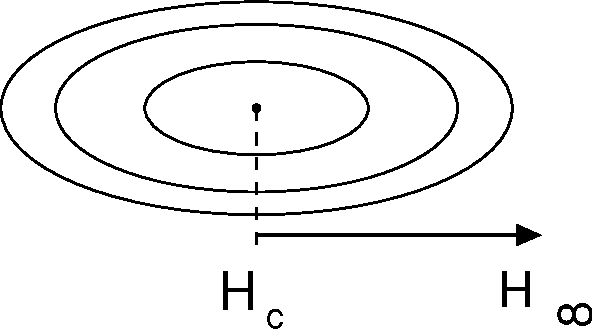
\includegraphics[width=\textwidth*7/8]{figures/classical_sa}
\caption{Depiction of the relation between the 2-D phase space of a Hamiltonian system with a single elliptic fixed point and the reduced space, a line segment.}
\label{f:classical reduction}
\end{center}
\end{figure}

\begin{figure}
\begin{center}
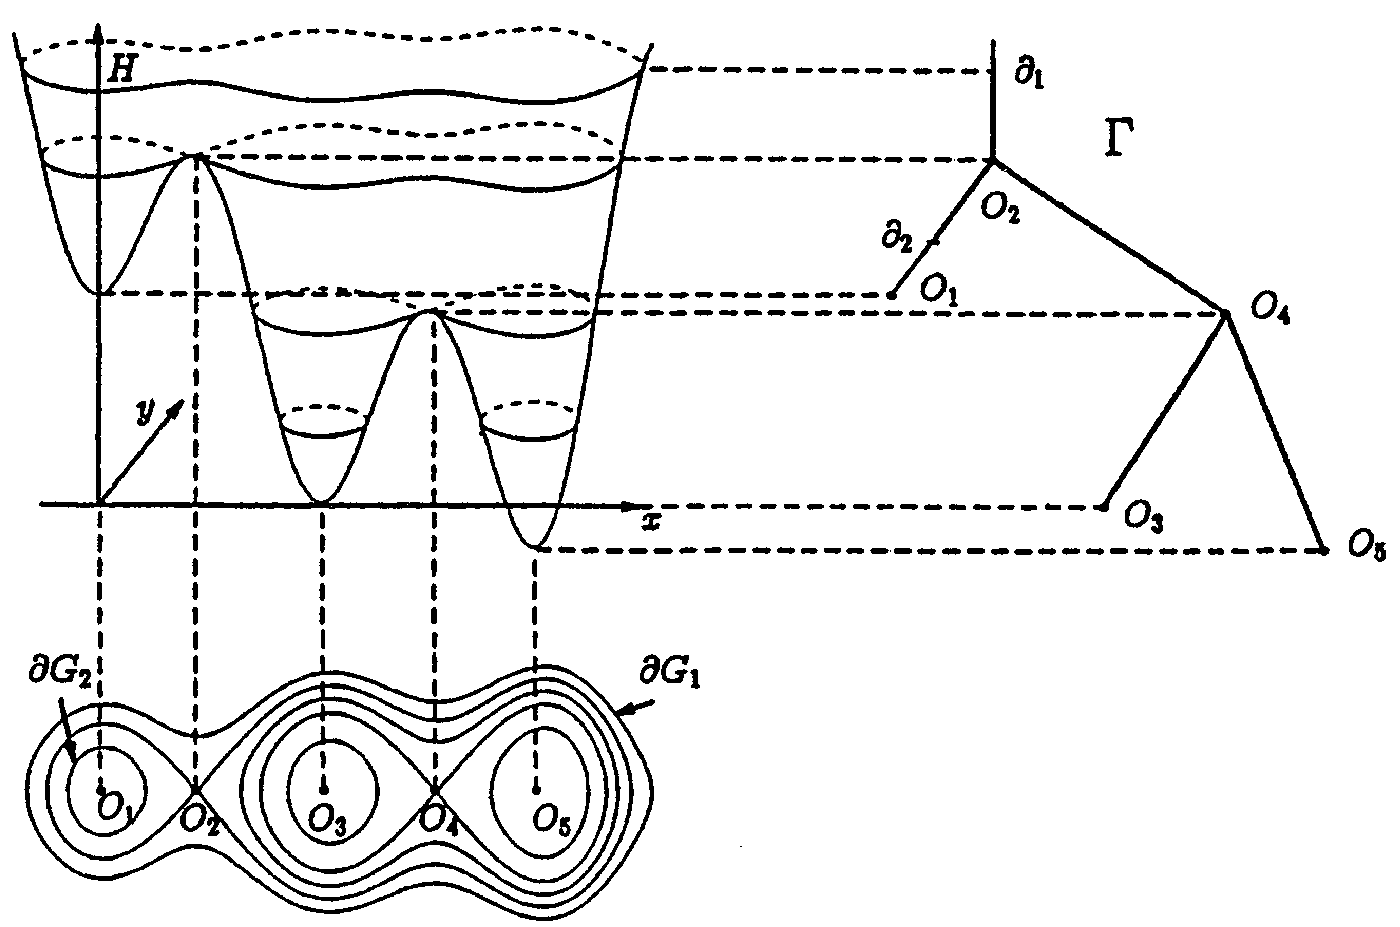
\includegraphics[width=\textwidth*7/8]{figures/graph_reduction_freidlin_weber}
\caption{Depiction of the relation between the 2-D phase space of a Hamiltonian system with multiple fixed points and the corresponding reduced graph. Figure reproduced from \citet{freidlin98:_random_pertur_nonlin_oscil}.}
\label{f:graph reduction}
\end{center}
\end{figure}

The reduced space of the problems studied in this thesis is two dimensional. Line segments seen in Figures \ref{f:classical reduction} and \ref{f:graph reduction} then become planes and the terminology of reduction on an open book \cite{freidlin04:_diffus} is introduced. Specific open book geometries will be given in \ref{s:unperturbed structure} and \ref{S:Unperturbed}, but here a general description is presented, in part to introduce notation.

The phase space of the systems we consider is composed  of elliptic and saddle fixed points, $\mathfrak{c}_i$, closed orbits with arbitrarily large values of $I$ where the process is killed $\BDY_i$ and open leaves, $\Gamma_i$ within which classical averaging results are valid. The union of these three components forms the graph of the reduced process:
\[
\Graph \equiv \bigcup_{i=1}^{N} \Gamma_i \cup \bigcup_{i=1}^{N_c}
[\mathfrak{c}_i] \cup \bigcup_{i=1}^{N_b}\BDY_i.
\]

\subsection{Main Results}

The dynamics of $y$ will deviate from those of $z$ noticeably only on time scales of order $\epsilon^{-1}$, thus time is rescaled such that $X^\epsilon_t \equiv x^\epsilon_{t/\epsilon^2}$. The fast dynamics are then governed by
\begin{equation}
\label{e:fast sde}
d X^\epsilon_t = \frac{1}{\epsilon} b^1 (X^\epsilon_t, t/\epsilon^2) dt + b^2 (X^\epsilon_t,t/\epsilon^2) dt + \frac{1}{\epsilon} g(X^\epsilon_t,t/\epsilon^2) dt
\end{equation}
and the slow dynamics are governed by
\begin{equation}
\label{e:slow sde}
dY^{\epsilon}_t = \frac{1}{\epsilon} F^1(X^\epsilon_t,t/\epsilon^2) dt + F^2(X^\epsilon_t,t/\epsilon^2) dt + \frac{1}{\epsilon} G(X^\epsilon_t,t/\epsilon^2) dt.
\end{equation}
The coefficients of the slow equation are found using the chain rule and Ito's formula (i.e. the stochastic chain rule), specifically,
% Formulas below are the standard chain rule, which is valid for real noise forcing. Do the formulas change if white noise forcing is used?
\begin{equation}
\label{e:slow sde coefficients}
\begin{aligned}
F^1_1& = \sum^4_{i = 1} \frac{\partial K}{\partial x_i} b^1_i& F^1_2& = \sum^4_{i = 1} \frac{\partial I}{\partial x_i} b^1_i\\
F^2_1& = \sum^4_{i = 1} \frac{\partial K}{\partial x_i} b^2_i& F^2_2& = \sum^4_{i = 1} \frac{\partial I}{\partial x_i} b^2_i\\
G_1& = \sum^4_{i = 1} \frac{\partial K}{\partial x_i} g_i&
G_2& = \sum^4_{i = 1} \frac{\partial I}{\partial x_i} g_i
\end{aligned}
\end{equation}
Note that $\Tave[b^1] = \bar \nabla K$, therefore
\[
\Tave[F^1_1] = \nabla K \cdot \bar \nabla K.
\]
Since the gradient and symplectic gradient produce vectors perpendicular to each other, $\Tave[F^1_1] = 0$. Similarly $\Tave[F^1_2] = 0$, therefore it starts to become evident that the dynamics of Equation \eqref{e:slow sde} are an order of $\epsilon$ slower than those of Equation \eqref{e:fast sde}.

This demonstrates that the dynamics of $Y_t^\epsilon$ are indeed slow compared to those of $X_t^\epsilon$.

For all problems treated in this thesis, it is a given that the fast process is a Markov process, which is to say a process for which the future is independent of everything but the present (delay differential equations do not satisfy this property.) Equation \eqref{e:fast sde} has a generator (\citep[\S 7.3]{øksendal03:_stoch_differ_equat}). For $\phi \in C^2(\reals^4 \times \reals)$ this generator is:
\[
(\gen^\epsilon \phi)(x,t) = \epsilon^{-1} (b^1,\nabla \phi)(x,t) + (\gen \phi)(x,t)
\]
where
\[
(\gen \phi)(x,t) = \sum_{i = 1}^4 b_i^2(x,t) \frac{\partial \phi}{\partial x_i}(x) + \frac12 \sum_{i,j=1}^4 a_{ij}(x,t) \frac{\partial^2 \phi}{\partial x_i \partial x_j}(x)
\]
where $a_{ij}(x,t) \equiv (g(x,t) g^T(x,t))_{ij}$. The theory of stochastic averaging provides the formalism required to prove that in the limit of infinitesimally small $\epsilon$, the generator for
$Y_t^\epsilon$ becomes decoupled from $X_t^\epsilon$. Effectively then, averaging becomes a method for dimensional reduction since a system in $\reals^4$ is approximated by one in $\reals^2$. Formally this result holds for infinitesimally small $\epsilon$.

The problem has now been setup to apply stochastic averaging theory. First, the results of stochastic averaging theory are stated and then the methods used to arrive at those results is explained. It must be noted that proofs for the results given below are not provided in this thesis, although in \citet{namachchivaya01:_unified_approac_noisy_nonlin_mathieu_type_system} similar results are proved. The principal difference between results in that reference and those used in this thesis is that in the reference, reduction from $\reals^2 \to \reals$ is analyzed, whereas here, the case of reduction from $\reals^4 \to \reals^2$ is treated. While this difference should not lead to significant changes, strictly speaking, the stochastic averaging formulas given below should be termed conjectures.

To begin, an averaging operator is defined.
\begin{definition}[Hamiltonian orbit averaging operator]
\label{d:Aave}
For a function $\varphi \in C^\infty(\reals^4)$, define averaging operator acting over Hamiltonian orbits, $\Aave$ by
\[
(\Aave \varphi) (y) \equiv \frac{1}{\period(y)} \int_0^{\period(y)} \varphi(z_s(x)) ds
\]
where $T(y)$ is the period associated with a Hamiltonian orbit.
\end{definition}

The reduced Markov process is defined in terms of its drift and diffusion coefficients. These two quantities are given by the following definition.
\begin{definition}[Averaged drift \& diffusion coefficients]
\begin{gather}
\mathfrak{b}_i(y) \equiv \left(\Aave \left(\Tave \left(F_i^2 + \mathfrak{f}_i + \mathfrak{g}_i\right)\right)\right)(y)\label{e:drift}\\
\Aa_{ij}(y) \equiv \left(\Aave \left(\Tave \left(\sigma\sigma^T\right)_{ij}\right)\right)(y)\label{e:diffusion}
\end{gather}
for $i,j = 1,2$, where
\[
\mathfrak f_i(x,t) \equiv \sum_{j=1}^4 \frac{\partial F_i^1(x,t)}{\partial x_j} \tilde f_j^1(x,t)
\]
\[
\tilde f_i^1 (x,t) \equiv \int_0^t \left\{b_i^1 (x,s) - \Tave_s (b_i^1(x,s)) \right\} ds\\
\]
\[
\mathfrak g_i(x,t) \equiv \int_{-\infty}^0 \Expectation \left[ \frac{\partial G_i (x,t,\xi_t)}{\partial x_j} g_j(x,t+\tau,\xi_{t+\tau}) \right] d\tau
\]
\[
\left(\sigma\sigma^T\right)_{jk}(x,t) \equiv \int_{-\infty}^\infty
\Expectation \left[G_j(x,t,\xi_t) G_k (x, t + \tau, \xi_{t+\tau}) \right] d\tau
\]
\end{definition}
It's worth pointing out that classical stochastic averaging theory, i.e. \citet{khasminskii68:_ito} is sufficient to provide these results since they hold within the leaves of the reduced domain, where one need not deal with fixed points and infinite periods.

\begin{definition}[Generator of the reduced Markov process]
\label{d:reduced generator}
The generator of the reduced Markov process is, for a function $f \in
C^2(\reals^2)$,
\[
(\gen_i^\dagger f)(y) = \sum_{j=1}^2
\mathfrak{b}^i_j(y) \frac{\partial f(y)}{\partial y_j} +
\frac12 \sum_{j,k = 1}^2 \mathfrak{a}^i_{jk}(y)
\frac{\partial^2 f(y)}{\partial y_j \partial y_k}
\]
$\mathfrak{b}$ is the drift coefficient and $\mathfrak{a}$ the diffusion coefficient. The domain of the generator of the process evolving on a $\mathfrak{G}$ with $n$ leaves is defined by
\begin{multline}
\mathfrak{D}_\mathfrak{G}^\dagger = \{f \in C(\mathfrak{G}) \cap
C^2(\bigcup_{i=1}^n \Gamma_i): \lim_{y \to \mathfrak c_i} (\gen^\dagger_i f)(y) \text{ exists}, \lim_{y \to \BDY_i} (\gen^\dagger_i f)(y) = 0 \quad \forall\, i,\\
\sum_{i=1}^n \{\pm\} \sum_{j=1}^2 \Bigl\{\sum_{k=1}^2
\mathring{\mathfrak a}^i_{jk}(\mathcal{O}) \frac{\partial f}{\partial
y_k}\bigg|_\mathcal{O} \Bigr\} \cdot \nu_j(\mathcal O) =0 \}
\label{e:generator domain}
\end{multline}
where $\mathring{\mathfrak{a}}$ denotes the same coefficient as in equation \eqref{e:diffusion} except that the $\Aave$-averaging operator excludes division by the period and $\mathcal O$ denotes the gluing vertex.
\end{definition}

The sum involving $\mathring{\mathfrak a}$ constitutes the gluing condition. An intuitive interpretation of the gluing condition is provided in \citet{namachchivaya01:_unified_approac_noisy_nonlin_mathieu_type_system}. This interpretation is extended to two-dimensions here. Define
\[
\alpha = \sum_{i=1}^n \lVert \mathring{\mathfrak a}^i(\mathcal{O}) \rVert.
\]
Suppose the limiting process starts on the page $\Gamma_1$. It will evolve according to $\gen_1^\dagger$ until it hits the gluing vertex. The process will then return to page $\Gamma_1$ with probability $\lVert \mathring{\mathfrak a}^1(\mathcal{O}) \rVert/\alpha$ and it will go to page $\Gamma_i$ with probability $\lVert \mathring{\mathfrak a}^i(\mathcal{O}) \rVert/\alpha$.

Now, a sketch is given for the proof that $\gen^\dagger$ is the generator of a Markov process and Equation \eqref{e:generator domain} its domain.
% FIXME Wiener vs. Brownian process
The Wiener process of the fast process given in Equation \eqref{e:fast sde} is given on the \emph{original} probability space, $(\Omega^o,\filt^o,\prob^o)$, where $\Omega^o$ is the event space, $\filt^o$ the filtration, and $\prob^o$ the probability measure. A \emph{canonical} space is introduced so as to transfer the dependence on $\epsilon$ from the process onto the measure. The original and canonical spaces are related by
\[
\prob^\epsilon(A) \equiv \prob^o(X^\epsilon \in A), \quad A \in B(\Omega)
\]
where $B(\Omega)$ denotes the space of Borel measures on $\Omega$.

The martingale problem is used because it gives an alternative formulation for the existence and uniqueness of weak solutions of stochastic differential equations (SDEs). Classical existence and uniqueness properties of are proved using Holder continuity of the SDE's coefficients, but such conditions are too strong to deal with the topology of the reduced space, which consists of leaves with edges that have singularities due to the homoclinic structure of the fast deterministic dynamics. Formally, the martingale problem is stated as follows \citep{rogers00:_diffus_markov}. Denote an SDE by:
\[
dX = b(X,t) dt + \sigma(X,t) dW
\]
Suppose $X$ is a weak solution to this equation starting at $y \in \reals^n$. Let $\prob^y$ be the law of $X$; $\prob^y$ is a probability measure on $(\Omega^n,\filt_t^n)$. Then $\prob^y$ has the following properties
\begin{enumerate}
\item $\prob^y(x_0 = y) = 1$
\item under $\prob^y$, for each $f \in C^\infty(\real^n)$
\[
M_t^f \equiv f(x_t) - f(x_0) - \int_0^t L f(x,s) ds
\]
where $L$ denotes the SDE's generator, is an $\filt_t^n$ martingale.
\end{enumerate}

For the fast process, $X_t^\epsilon$, the existence and uniqueness of weak solutions is assured by the fact that \eqref{e:fast sde} is a well-behaved SDE. Thus, by the martingale problem we can state that, for $f \in C^2(\reals^4 \times \reals)$ a function $2\pi$-periodic in its last argument,
\[
M_t^{f,\epsilon} \equiv f(X_t,t/\epsilon^2) - \int_0^t \epsilon^{-2} \frac{\partial f}{\partial s}(X_s,s/\epsilon^2) + (\gen^\epsilon f)(X_s,s/\epsilon^2) ds,
\]
% FIXME Where does the \order(\epsilon^{-2}) term come from?
is a martingale with respect to the filtration ${\filt_t; t \geq 0}$ under the probability measure $\prob^\epsilon$. An alternative form of the martingale problem is used in proofs \citep{ethier86:_markov_process}. If $0 \leq r_1 < r_2 \dots < r_n \leq s < t$ and ${\phi_j; j = 1,2 \dots n} \in C_b(\reals^n)$, then
\begin{multline*}
\Expectation^\epsilon \Big[\Big\{f(X_t) - f(X_s) - \int_s^t \epsilon^{-2} \frac{\partial f}{\partial s}(X_u,u/\epsilon^2) \\
+ (\gen^\epsilon f)(X_u,u/\epsilon^2) du\Big\} \prod_{j=1}^{n} \phi_j(X_{r_j})\Big] = 0.
\end{multline*}
This form of the martingale property relies on the fact that functions of the form $\prod_{j=1}^n \phi_j(X_{r_j})$ generate $\filt_s$.

Stochastic averaging theory show that the law of the reduced process, $Y^\epsilon_t$, converges to a unique limit. This is also stated in a canonical space. $Y^\epsilon_t$ takes values in $\Graph$. The event space is $\Omega^\dagger \equiv C([0,\infty),\Graph)$, the filtration is $\filt^\dagger$ and the canonical probability measure is defined by
\[
\prob^{\epsilon,\dagger} \equiv \prob^{\epsilon}(Y \in A),\quad A \in B(\Omega^\dagger).
\]
Stochastic averaging theory is used to prove the existence and uniqueness of the limit
\begin{equation}
\label{e:limit def}
\prob^\dagger \equiv \lim_{\epsilon \to 0} \prob^{\epsilon,\dagger}.
\end{equation}
Formally, the main theorem of stochastic averaging is stated as follows. $\prob^{\epsilon,\dagger}$ tends to a unique solution $\prob^\dagger$ of the martingale problem with generator $\gen^\dagger$ and with initial condition $\delta_{y_0}$. This means $\prob(Y_0^\dagger = Y_0) = 1$, and if $f \in \mathfrak{D}_\mathfrak{G}^\dagger$, $0 \leq r_1 < r_2 \dots < r_n \leq s < t$ and ${\phi_j^\dagger; j = 1,2 \dots n} \in C(\Graph)$, then
\begin{equation}
\label{e:sa main}
\Expectation^\dagger \left[\left\{f(Y_t^\dagger) - f(Y_s^\dagger) - \int_s^t (\gen^\dagger f)(Y_u^\dagger) du\right\} \prod_{j=1}^{n} \phi_j^\dagger(Y_{r_j}^\dagger)\right] = 0.
\end{equation}

% FIXME \gen^\dagger vs. \gen^\dagger_i
To prove that $\gen^\dagger$ is the generator of a Markov process, the first step is to show the reduced probability measure, $\prob^{\epsilon,\dagger}$ is tight in the Prohorov topology on $B(\Omega^\dagger)$. Then, by Prokhorov's theorem, there exists at least one cluster point in the weak topology of probability measures on $\Omega^\dagger$.

Based on definition \eqref{e:limit def}, \eqref{e:sa main} can be stated as
\[
\lim_{\epsilon \to 0} \Expectation^{\epsilon,\dagger} \left[\left\{f(Y_t^\dagger) - f(Y_s^\dagger) - \int_s^t (\gen^\dagger f)(Y_u^\dagger) du\right\} \prod_{j=1}^{n} \phi_j^\dagger(Y_{r_j}^\dagger)\right] = 0
\]
and reverting back to the unreduced process, the above can be stated as
\[
\lim_{\epsilon \to 0} \Expectation^\epsilon \left[\left\{f(Y_t) - f(Y_s) - \int_s^t (\gen^\dagger f)(Y_u) du\right\} \prod_{j=1}^{n} \phi_j(Y_{r_j})\right] = 0.
\]
In the original canonical space, it's known that, if $y = \mathcal R(x,y)$,
\[
\Expectation^\epsilon \left[\left\{f(Y_t) - f(Y_s) - \int_s^t (\gen^\epsilon (f \circ \mathcal R))(X_u) du\right\} \prod_{j=1}^{n} \phi_j(X_{r_j})\right] = 0
\]
for all $\epsilon > 0$. This demonstrates that the bulk of the work that needs to be performed to prove stochastic averaging results is to show
\[
\lim_{\epsilon \to 0} \Expectation \left[\left| \left(\int_0^t (\gen^\epsilon (f \circ \mathcal R))(X_s) - (\gen^\dagger f)(Y_s)\right) du \right|\right] = 0.
\]
Denoting
\[
(\gen^\epsilon (f \circ \mathcal R))(x,t) = L^\epsilon_1(x,t) + L^\epsilon_2(x,t)
\]
where
\[
\begin{aligned}
L^\epsilon_1(x,t) &\equiv (\gen K)(x,t) \frac{\partial f^\epsilon}{\partial K} (K(x),I(x)) + (\gen I)(x,t)\frac{\partial f^\epsilon}{\partial I} (K(x),I(x))\\
&\quad + \frac12 \Big\{\langle dK,dK \rangle(x,t) \frac{\partial^2 f^\epsilon}{\partial k^2} (K(x),I(x))\\
&\quad + \langle dI,dI \rangle(x,t) \frac{\partial^2 f^\epsilon}{\partial i^2} (K(x),I(x))\Big\}\\
&\quad + \langle dK,dI \rangle(x,t) \frac{\partial^2 f^\epsilon}{\partial k \partial i} (K(x),I(x))\\
\end{aligned}
\]
and
\begin{multline*}
L^\epsilon_2(x,t) \equiv \frac{1}{\epsilon} \Big\{( b^1, \nabla K)(x,t)\frac{\partial f^\epsilon}{\partial k}(K(x),I(x))\\
+ (b^1, \nabla I)(x,t)\frac{\partial f^\epsilon}{\partial i}(K(x),I(x))\Big\}
\end{multline*}
for all $x \in \reals^4$ and $t \ge 0$. The fastest variation is the oscillation of coefficients, which has period $\epsilon^2$; the second-fastest variation is the motion around the orbits of $z$; these oscillations have period $\epsilon$. Thus we should have
\[
\int_0^t L^\epsilon_1(X_u,u/\epsilon^2)du \approx \int_0^t (\Tave L^\epsilon_1)(X_u)du \approx \int_0^t(\Aave \Tave L^\epsilon_1)(K(X_u),I(X_u)) du.
\]
It should be possible to prove this using standard averaging techniques, as was done for reduction from $\reals^2 \to \reals$ in \citet{namachchivaya01:_unified_approac_noisy_nonlin_mathieu_type_system}.
The analysis of $L^\epsilon_2$ is a bit more delicate since it contains large fluctuations, which are of order one on average.

\section{Thesis Outline}

The remainder of this thesis is organized as follows. Chapter \ref{c:oscillator} applies stochastic averaging techniques to a resonant periodically driven noisy oscillator. This is problem where the original system is two-dimensional and the reduced system is one dimensional. Thus the averaging analysis can be done without recourse to numerical techniques. In this sense, Chapter \ref{c:oscillator} serves as an introductory example. This chapter is self-contained.

In Chapter \ref{c:sgwaves} a model of surface wave motion will be analyzed. This is perhaps the most challenging application of stochastic averaging in this thesis. The first step is to transform partial differential equations into an infinite system of ordinary differential equations. The graph of the reduced process has a relatively complicated geometry and in order to calculate averaged drift and diffusion coefficients, numerical algorithms are devised.

In Chapter \ref{c:autoparametric} an autoparametric oscillator model will be analyzed. The level of complexity of this problem is similar to the wave motion problem, however more calculations can be done analytically, simplifying the analysis slightly.

In Chapter \ref{c:pdf}, the main results of this thesis are developed. Stationary probability density solutions are given for the surface wave and autoparametric problems. These solutions are found with a finite-element method (FEM). In Chapter \ref{c:pdf}, a sample path method is also developed to solve the Fokker--Planck equation. This serves to validate the FEM.

Chapter \ref{c:conclusions} concludes the thesis. In that chapter, results are summarized and possible extensions to the work in this thesis are presented.

%% Classical vs. non-standard stochastic averaging: 2-D problems, third time scale, bifurcations and martingale problem and gluing condition

%%% Local Variables: 
%%% mode: latex
%%% TeX-master: "main"
%%% End: 


\chapter{Resonant Dynamics of a Periodically Driven Noisy Oscillator}
\label{c:oscillator}
\section{Introduction}
\label{sec:intro}

We are interested in the nonlinear response of a single-degree-of-freedom system under both \emph{periodic} and \emph{stochastic} external excitations. The general form of the equations studied here is given by

\begin{equation}
\ddot q_t + \frac{\partial U}{\partial q}(q_t) + G(q_t, \dot q_t) \dot q_t
= \mu_0 \cos(\omega t) + \mu_1 \xi(t),
\label{E:geom}
\end{equation}
where $q \in \reals$ represents a generalized coordinate and the potential $U: \reals \to \reals$ has a single well. More precisely, we require that $U \in C^\infty(\reals; \reals_+)$, that $\lim_{|x|\to\infty}U(x) = \infty$, that
\[
\{x \in \reals: U^\prime(x) = 0\} = \{x \in \reals: U(x)=0\} = 0,
\]
and that $\omega_0^2 \equiv U^{\prime \prime}(0)>0$. See Figure~\ref{F:Pot}.
\begin{figure}
\begin{equation*}
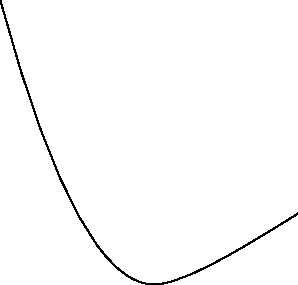
\includegraphics[width=\textwidth*1/3]{figures/pot}
\end{equation*}
\caption{Potential energy}
\label{F:Pot}
\end{figure}

In~\eqref{E:geom}, $G$ represents dissipative terms, and $\xi$ represents mean zero, stationary, independent Gaussian white noise processes. For convenience, we shall define
\[
U_h(q) \equiv U(q) + \frac12 \omega_0^2 q^2. \qquad q \in \reals
\]
Since an exact solution of~\eqref{E:geom} is not known, the purpose of the present analysis is to develop a stochastic averaging technique of perturbed two-dimensional Hamiltonian systems with an elliptic fixed point. The analytical methods presented are based on \citet{freidlin98:_random_pertur_nonlin_oscil, namachchivaya01:_unified_approac_noisy_nonlin_mathieu_type_system, namachchivaya02:_rigor_stoch_averag_center_addit_noise, sowers03:_stoch_averag_near_homoc_orbit}.

Introducing appropriate scaling of parameters for the nonlinear, dissipative, and time dependent terms, we recast~\eqref{E:geom} as
\begin{equation}
\ddot q_t^\epsilon + \omega_0^2 q_t^\epsilon + \epsilon^n \frac{\partial U_h}{\partial q}(q_t^\epsilon) + \epsilon^d G(q_t^\epsilon,\dot q_t^\epsilon) \dot q_t^\epsilon = \epsilon \mu_0 \cos(\omega t) + \epsilon^\nu \mu_1 \xi(t),
\label{E:geom_scale}
\end{equation}
Our interest is the behavior of $q$ in a certain \emph{limiting regime}. Depending on the values of $n,d,\nu$, the limiting dynamics of the state $(q^\epsilon,\dot q^\epsilon)$ as $\epsilon \to 0$ are significantly different. In \citet{namachchivaya01:_unified_approac_noisy_nonlin_mathieu_type_system} a unified approach for noisy weakly nonlinear systems like~\eqref{E:geom_scale} was developed for the case when $n=1$. Here, by appropriate scaling of the nonlinear term $\partial U_h/\partial q$, the solution $(q^\epsilon,\dot q^\epsilon)$ over any finite interval converges in probability, as $\epsilon \to 0$, to the solution of an averaged equation which has a conservation law. The averaged equation has certain nontrivial (yet generic) types of fixed points. The evolution of the first integral (associated with a conservation law) was examined on a rescaled time interval.

A number of researchers have worked on Duffing oscillators in various environments. In the absence of noisy perturbations (i.e., $\mu_1=0$), equation~\eqref{E:geom_scale} represents a harmonically forced nonlinear oscillator. This has been studied extensively \citep{guckenheimer83:_nonlin, nayfeh79:_nonlin_oscil}. On the other hand, in the absence of periodic perturbations (i.e., $\mu_0 = 0$),~\eqref{E:geom_scale} represents the noisy \emph{Duffing-van der Pol} equation which has been studied by \citet{arnold96:_towar_hopf, liang99:_stoch_dynam, lin67:_probab_theor_struc_dynam} and \citet{bolotin84:_random}, to name a few. Here the work of \citet{namachchivaya01:_unified_approac_noisy_nonlin_mathieu_type_system} is extended to include more general (strongly) nonlinear systems ($n=0$ in~\eqref{E:geom_scale}) and obtain analytical results for a low-dimensional model of~\eqref{E:geom_scale}. \emph{Stochastic averaging} can achieve model-reduction for two different sets of values of $d$ and $\nu$. Here, we consider the case in which the order of the noise equals that of the dissipation, i.e., $d = \nu = 1$. Note that when the noise intensity is larger than the dissipative or periodic perturbations, i.e., $\nu=1/2$, it becomes possible to use the results of \citet{pinsky88:_lyapun}. Pinsky-Wihstutz scaling stretches the coordinates in such a way that to leading order, stochastic forcing induced diffusion balances dissipative drift.

It is well known that stochastic resonance (SR) can arise in under-damped systems with a single-well potential, unlike \emph{conventional} SR in multi-well potentials. Therefore, to study such SR, we shall consider a prototypical single-well potential
\[
U(q) = \frac12 q^2 + \frac14 q^4 + Bq
\]
with two distinct cases depending on the constant $|B|$. In the first case, when $|B| \le B_c$ the nonlinear oscillation frequency $\Omega(E)$ monotonically increases with total energy $E$ as shown in Figure~\ref{F:frequency}(a). In the second case with $|B| > B_c$, the system frequency $\Omega(E)$ is non-monotonic as sketched in Figure~\ref{F:frequency}(b). Furthermore, in the absence of the periodic forcing, the under-damped oscillator exhibits the so-called sharp \emph{zero-dispersion spectral peaks} (ZDPs) close to the extremal frequency $\Omega_m$ in the fluctuation spectrum. The magnitude of the ZDP climbs up exponentially with increasing noise strength $\mu_1$. The extreme narrowness of the ZDP~\citet{soskin89:_fluct, soskin92:_evolut} suggests that stochastic resonance in the latter case is far more dramatic phenomenon than in the former case. Here, we investigate the system with a symmetric single potential, i.e., $B=0$ and the constant damping coefficient, $G(q^\epsilon_t,\dot q_t^\epsilon) = \zeta$. Thus Equation~\eqref{E:geom_scale} becomes
\[
\ddot q_t^\epsilon + \epsilon \zeta \dot q_t^\epsilon + q_t^\epsilon + {q_t^\epsilon}^3 = \epsilon \mu_0 \cos (\omega t) + \epsilon \mu_1 \xi(t)
\]

In section~\ref{S:problem setup} is devoted to setting up a framework to study the effect of random perturbation of the system near the resonance surface. In other words, adequately scaled local coordinates adjacent to the resonance surface are introduced from the system in action space. In section~\ref{S:reduction}, a cascaded averaging approach is presented for the local system under the capture into resonance. More specifically, we address a separation of time scales so that state variables of fast time scale can be averaged out while the equation of the slow variable is approximated. The near resonant motion is reduced to a graph valued process which turns out to converge weakly to a Markov process with a limiting generator. Section~\ref{S:stationary pdf} presents stationary probability density from the limiting generator which characterize the reduced Markov process. In the final section, we give conclusion and conjecture regarding the effect of SR.

\section{Problem Setting}
\label{S:problem setup}

By making use of the system Hamiltonian with strong nonlinear terms, we write~\eqref{E:geom} with the standard rescaling for dissipation, as a weakly perturbed Hamiltonian system
\begin{equation}
\begin{aligned}
\dot x_t^\epsilon &= \frac{\partial {\mathcal H}(x_t^\epsilon,y_t^\epsilon)}{\partial y}\\
\dot y_t^\epsilon &= -\frac{\partial {\mathcal H}(x_t^\epsilon,y_t^\epsilon)}{\partial x} + \epsilon F^y (x_t^\epsilon, y_t^\epsilon, \theta_t) + \epsilon G^y(x_t^\epsilon, y_t^\epsilon) \xi(t)\\
\dot \theta_t &= \omega,
\end{aligned}
\label{E:eom-qp-eps}
\end{equation}
where $(x_0^\epsilon, y_0^\epsilon)\equiv(x,y) \in \reals^2$, $\theta_0 \equiv \theta \in S$. The unperturbed ($\epsilon = 0$) equations corresponding to~\eqref{E:eom-qp-eps} form a Hamiltonian
\[
\mathcal H (x,y) = \frac{y^2}{2} + U (x)
\]
where $U(x) = x^2/2+x^4/4$. We apply a canonical transformation to obtain new variables $\phi, I$ in such a way that the transformed Hamiltonian remains a constant, $I$, and the angle $\phi$ increases by one during every period of rotation. The conjugate momentum corresponding to $\phi$ is the action $I$. Thus, the unperturbed integrable Hamiltonian equations with elliptic fixed points can be written as
\begin{align}
\dot I_t &= 0, & \dot \phi_t &= \Omega (I_t), & \dot \theta_t &= \omega,
\label{E:eom-aca-zero}
\end{align}
and the perturbed equations \eqref{E:eom-qp-eps} simplify to the following Stratonovich equations
\begin{equation}\begin{aligned}
d I_t^\epsilon &= \epsilon f^I(I_t^\epsilon, \phi_t^\epsilon, \theta_t) dt + \epsilon g^I (I_t^\epsilon, \phi_t^\epsilon) \circ dW_t\\
d \phi_t^\epsilon &= \Omega(I_t^\epsilon) dt + \epsilon f^\phi (I_t^\epsilon, \phi_t^\epsilon, \theta_t) dt+ \epsilon g^\phi (I_t^\epsilon, \phi_t^\epsilon) \circ dW_t\\
d \theta_t &= \omega d t,
\end{aligned}\label{E:eom-aca-eps}
\end{equation}
where $I_0=I \in \reals, \phi_0 = \phi \in S, \theta_0=\theta \in S$. $S$ denotes the circle with unit radius in 2-dimensional Euclidean space. We shall use the dominant global dynamics and the \emph{phase-space stratification} of~\eqref{E:eom-aca-zero} to capture the long-term behavior of the dissipative, periodically driven, noisy system~\eqref{E:eom-aca-eps}.

As stated in the introduction, our principal technique of dimensional reduction will be the method of stochastic averaging for nonlinear systems with small noise. As the noise becomes asymptotically small, one can exploit separation of scales to find an appropriate lower-dimensional description of the system for many important random vibration problems. The unique feature in our treatment will be the inclusion of resonances, as we shall describe below.

\subsection{Resonances in Two Frequency System}

In an integrable Hamiltonian system such as~\eqref{E:eom-aca-zero}, if the frequencies are non-commensurable, then the orbits are everywhere dense on $S^2$ and the motion corresponding to the unperturbed system~\eqref{E:eom-aca-zero} is called \emph{quasi-periodic}. Resonance occurs when the frequencies are commensurable or nearly commensurable, and the closure of an orbit is a one-dimensional torus. Since $\Omega$ depends on the action $I$, the resonance will depend on certain values of the action.

\begin{definition}[Resonance]
For the two-phase system, resonances occur when $\Omega$'s, are connected by a commensurability relation
\begin{align}
\kappa_1 \,\Omega(I) + \kappa_2 \, \omega &= 0, & \kappa &= (\kappa_1,\kappa_2) \in \integers^2 - (0,0)
\label{E:resonance}
\end{align}
and the order of the resonance is given by $|\kappa| = \sum_{i=1}^2 \kappa_i$.
\end{definition}
If we regard $(\kappa_1,\kappa_2) \in \integers^2 -(0,0)$ as fixed, then~\eqref{E:resonance} is a single equation in one unknown. Away from the equilibrium point~($\Omega(I) \neq 0$) and at a particular value $I^{m:n}$ with $(\kappa_1,\kappa_2)=(m,-n)$, we have
\[
\frac{\Omega(I^{m:n})}{\omega} = \frac{n}{m} \in \rationals
\]
So each rational value assumed by the above frequency ratio corresponds with a resonance domain, in principal, an infinite number of such resonance domains exist.
\begin{definition}[Resonance Module: $\Omega^{\perp}$]
For some fixed $I$, the resonance module is a 2-dimensional integer vector
\[
\Omega^{\perp} \equiv \{ \kappa = (\kappa_1,\kappa_2) \in \integers^2 - (0,0): \kappa_1 \Omega(I) + \kappa_2 \omega = 0 \}
\]
\end{definition}
\begin{definition}[Resonance Set: $\reals_k$]
The resonance set are those values of $I$ for which a particular resonance $\kappa = (m,-n) \in \integers^2 - (0,0)$ occurs, i.e.,
\[
\reals_k \equiv \{ I \in \dom \subset \reals^2: \kappa_1 \Omega(I) + \kappa_2 \omega  = 0, \kappa = (\kappa_1,\kappa_2) \in \integers^2 - (0,0) \}
\]
\end{definition}
A resonance set is a point in the one-dimensional action space and this point along with the variables $(\phi, \theta) \in S^2$ forms, what is often called a resonance surface.
\begin{figure}[htbp]
\centering
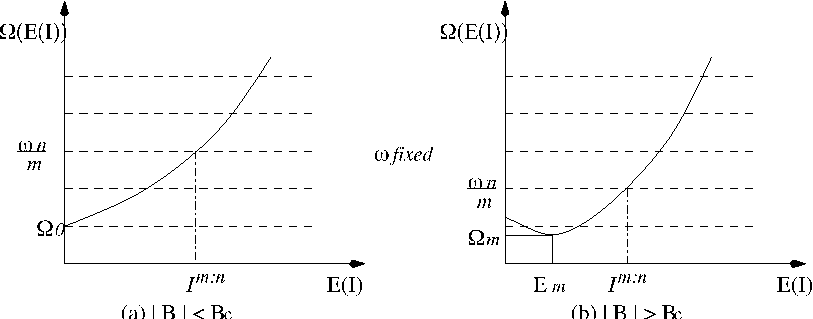
\includegraphics[width=\textwidth]{figures/freq}
\caption{Resonance sets for the Duffing equation}
\label{F:frequency}
\end{figure}
For some fixed $(\kappa_1,\kappa_2) = (m,-n)$, the resonance set for the Duffing equation, for example, consists of just one point $I^{m:n}$. When the trajectory of a phase point arrives at this surface, the trajectory either passes through the resonance and gets away from the resonant surface or gets captured into resonance. The captured trajectory moves slowly while preserving the resonance condition and may leave the resonance surface after a time interval of order $\epsilon^{-1}$. In the next section we describe the perturbed stochastic dynamics of system~\eqref{E:eom-qp-eps} close to this resonance surface with the aim of determining the effects of noisy perturbations on the passage of trajectories through the resonance zone.

\subsection{Scaling Close to a Resonant Surface}
\label{S:scaling}

The near resonant motion of randomly perturbed integrable systems is not well understood. In this section, we will study this problem in depth by introducing local coordinates close to the resonance surface. A point ($I,\phi,\theta$) in the neighborhood of the resonant surface will be specified by $r$, the distance to the resonant surface, and the angles ($\gamma,\theta$). Since in the frequency plane, $\Omega(I)-\omega$, the resonance curve forms a straight line through the origin with the normal defined by $r \equiv m \Omega(I) - n \omega$. If we assume
\[
\frac{\partial \Omega}{\partial I} (I) \neq 0
\]
then the transformation is invertible, i.e. $I=I(r)$. Hence, we introduce a distance to the resonant manifold as
\[
\eta \equiv I - I^{m:n},
\]
Making use of~\eqref{E:eom-aca-zero} we introduce a slow angle $\gamma$
\[
m \dot \phi - n \dot \theta = \frac{d}{dt} \left(m \phi - n \theta \right) \equiv \frac{d \gamma}{dt}, \quad \text{for} \quad \kappa =(m,-n) \in \Omega^{\perp}.
\]
and it is clear that there is a 2$\times$2 matrix
\[
A = \left[
\begin{array}{cc} m & -n \\ 0 & 1 \\ \end{array} \right],
\]
with $m \neq 0$. The matrix $A$ satisfies $A \cdot \Omega = [0, \omega]^\text{T}$ and it can be used to transform between fast and slow variables since $A \cdot [\phi, \theta]^\text{T} = [\gamma, \theta]^\text{T}$. We can write the evolutions in the new variables $\eta_t^\epsilon,\gamma_t^\epsilon,\theta_t$ using the Taylor expansion, about $\eta = 0$ as
\begin{equation}
\begin{aligned}
d {\eta}_t^\epsilon &= \epsilon \left\{
f^I(I^{m:n},\phi_t^\epsilon(\gamma_t^\epsilon,\theta_t),\frac{\theta_t}{\omega}) + \frac{\partial f^I}{\partial I}(I^{m:n},\phi_t^\epsilon(\gamma_t^\epsilon,\theta_t),\frac{\theta_t}{\omega}) \, {\eta}_t^\epsilon \right.\\
&\quad \left. + \frac12 \frac{\partial ^2 f^I}{\partial I ^2}(I^{m:n},\phi_t^\epsilon(\gamma_t^\epsilon,\theta_t),\frac{\theta_t}{\omega}) \, ({\eta}_t^\epsilon)^2 \right\} + \epsilon \left\{g^I(I^{m:n}, \phi_t^\epsilon(\gamma_t^\epsilon, \theta_t)) \right.\\
&\quad \left. + \frac{\partial g^I}{\partial
I}(I^{m:n},\phi_t^\epsilon(\gamma_t^\epsilon,\theta_t)) \,
{\eta}_t^\epsilon + \frac12 \frac{\partial^2 g^I}{\partial I^2}(I^{m:n},\phi_t^\epsilon(\gamma_t^\epsilon,\theta_t)) \, ({\eta}_t^\epsilon)^2\right\} \circ dW_t\\
d {\gamma}_t^\epsilon &= m \frac{\partial \Omega}{\partial I}
(I^{m:n}) {\eta}_t^\epsilon +\frac{m}{2}\frac{\partial
^2\Omega}{\partial I^2} (I^{m:n}) ({\eta}_t^\epsilon)^2
 + \epsilon  m \left\{ f^{\phi}(I^{m:n},\phi_t^\epsilon(\gamma_t^\epsilon,\theta_t),\frac{\theta_t}{\omega}) \right.\\
&\quad + \left.\frac{\partial f^{\phi}}{\partial
I}(I^{m:n},\phi_t^\epsilon(\gamma_t^\epsilon,\theta_t),\frac{\theta_t}{\omega})
\, {\eta}_t^\epsilon+ \frac12 \frac{\partial^2 f^{\phi}}{\partial
I^2}(I^{m:n},\phi_t^\epsilon(\gamma_t^\epsilon,\theta_t),\frac{\theta_t}{\omega})
({\eta}_t^\epsilon)^2\right\}\\
&\quad + \epsilon m \left\{g^{\phi}(I^{m:n},\phi_t^\epsilon(\gamma_t^\epsilon,\theta_t))
+ \frac{\partial g^{\phi}}{\partial
I}(I^{m:n},\phi_t^\epsilon(\gamma_t^\epsilon,\theta_t)) \eta_t^\epsilon\right.\\
&\quad + \left.\frac12 \frac{\partial^2 g^{\phi}}{\partial I^2}(I^{m:n},\phi_t^\epsilon(\gamma_t^\epsilon,\theta_t)) ({\eta}_t^\epsilon)^2\right\} \circ dW_t\\
d {\theta}_t &= \omega d t \quad \text{where} \quad
\phi_t^\epsilon(\gamma_t^\epsilon,\theta_t)\equiv\frac{\gamma_t^\epsilon}{m}+\frac{n}{m}\theta_t
\end{aligned}
\label{E:pw}
\end{equation}
On the resonant surface $\eta=0$ and in the neighborhood of that surface $\eta$ is small, since the effect of a resonance is felt in a narrow strip about the resonance line called the \emph{resonant zone}. Due to the nilpotent structure of the zeroth order terms in equations~\eqref{E:pw}, we need an appropriate scaling to capture the dynamics in the proximity of the resonant zone. For the case of interest in the current analysis (i.e. noise intensity  of the same order as the dissipative perturbation) the width of the resonant zone is of order $\sqrt\epsilon a_k$ where $a_k$ is an upper bound for the amplitudes of the resonant harmonics of the perturbations. Accordingly, $\eta$ is rescaled:
\[
\eta = \epsilon^\frac12 h.
\]
Thus, we obtain the following set of stochastic equations from~\eqref{E:pw}
\begin{equation}
\begin{aligned}
d h_t^\epsilon &= \left\{\epsilon^{1/2} f^I_0\Big(I^{m:n},\phi_t^\epsilon(\gamma_t^\epsilon,\theta_t),\frac{\theta_t}{\omega}\Big)
 + \epsilon f^I_1 \Big(I^{m:n}, \phi_t^\epsilon(\gamma_t^\epsilon, \theta_t), \frac{\theta_t}{\omega}\Big) h_t^\epsilon \right\} dt\\
&\quad + \left\{\epsilon^{1/2} g^I_0(I^{m:n}, \phi_t^\epsilon(\gamma_t^\epsilon, \theta_t)) + \epsilon g^I_1(I^{m:n},\phi_t^\epsilon(\gamma_t^\epsilon,\theta_t)) {h}_t^\epsilon\right\} \circ dW_t\\
d \gamma_t^\epsilon &= m \left\{ \epsilon^{1/2} \frac{\partial \Omega}{\partial I} (I^{m:n}) {h}_t^\epsilon + \frac{\epsilon}{2}\frac{\partial^2 \Omega}{\partial I^2} (I^{m:n}) ({h}_t^\epsilon)^2 \right\} dt\\
&\quad + m \left\{ \epsilon f^\phi_0\Big(I^{m:n},\phi_t^\epsilon(\gamma_t^\epsilon,\theta_t),\frac{\theta_t}{\omega}\Big) + \epsilon^{3/2} f^{\phi}_1\Big(I^{m:n},\phi_t^\epsilon(\gamma_t^\epsilon,\theta_t),\frac{\theta_t}{\omega}\Big) h_t^\epsilon \right\} d t\\
&\quad + m \left\{\epsilon g^{\phi}_0(I^{m:n}, \phi_t^\epsilon(\gamma_t^\epsilon, \theta_t)) + \epsilon^{3/2} g^\phi_1(I^{m:n},\phi_t^\epsilon(\gamma_t^\epsilon,\theta_t)) h_t^\epsilon\right\} \circ dW_t\\
d {\theta}_t &= \omega dt
\end{aligned}\label{E:zrgp}
\end{equation}
It is important to realize that the scaled Stratonovich
equation~\eqref{E:zrgp} are the \emph{starting point} for the
rest of the analysis.

\section{Reduction to Graph Valued Processes}
\label{S:reduction}

Our goal in the first part of this section is to describe the perturbed stochastic dynamics of the system~\eqref{E:zrgp} close to this resonance surface for the case $\mu=1/2$. Keeping the first two orders in each equations of motion~\eqref{E:zrgp}, we get
\begin{equation}
\begin{aligned}
d h_t^\epsilon &= \left\{\epsilon^{1/2} f^I_0\Big(I^{m:n},\phi_t^\epsilon(\gamma_t^\epsilon,\theta_t),\frac{\theta_t}{\omega}\Big) + \epsilon f^I_1\Big(I^{m:n}, \phi_t^\epsilon(\gamma_t^\epsilon, \theta_t), \frac{\theta_t}{\omega}\Big) h_t^\epsilon \right\} dt\\
&\quad + \epsilon^{1/2} g^I_0(I^{m:n}, \phi_t^\epsilon(\gamma_t^\epsilon, \theta_t)) \circ dW_t\\
d \gamma_t^\epsilon &= m \left\{\epsilon^{1/2} \frac{\partial \Omega}{\partial I} (I^{m:n}) {h}_t^\epsilon + \epsilon f^\phi_0\Big(I^{m:n}, \phi_t^\epsilon(\gamma_t^\epsilon, \theta_t), \frac{\theta_t}{\omega}\Big) + \frac{\epsilon}{2} \frac{\partial^2 \Omega}{\partial I^2}(I^{m:n}) (h^\epsilon_t)^2 \right\} dt\\
&\quad + \epsilon  m g^\phi_0(I^{m:n}, \phi_t^\epsilon(\gamma_t^\epsilon, \theta_t)) \circ dW_t\\
d {\theta}_t &= \omega d t
\end{aligned}
\label{E:zrgp-case2}
\end{equation}
where
\begin{gather*}
f_0^I = \frac{\partial I}{\partial y} (\mu_0 \cos \omega t - \zeta y) = \frac{y}{\Omega(I)} (\mu_0 \cos \omega t - \zeta y),\\
f_1^I = \frac{\partial f_0^I}{\partial I}, \quad g_0^\phi = \mu_1 \frac{\partial \phi}{\partial y} = - \mu_1 \frac{\partial x}{\partial I},\\
g_0^I = \mu_1 \frac{\partial I}{\partial y} = \mu_1 \frac{\partial I}{\partial H}\frac{\partial H}{\partial y} = \frac{\mu_1}{\Omega(I)} y,\\
f_0^\phi = \frac{\partial \phi}{\partial y} (\mu_0 \cos \omega t - \zeta y) = -\frac{\partial x}{\partial I} (\mu_0 \cos \omega t - \zeta y).
\end{gather*}
Since this section deals with a fixed resonance band, we can easily express
\[
\phi_t^\epsilon(\gamma_t^\epsilon,\theta_t)= \Omega(I^{m:n}) t +  \frac{\gamma_t^\epsilon}{m} = \frac{\omega n}{m} t + \frac{\gamma_t^\epsilon}{m} \text{ and } \theta_t= \omega t
\]
Define $\tilde\epsilon\equiv{\sqrt{\epsilon}}$. We can then rewrite \eqref{E:zrgp-case2} as the Ito stochastic differential equation,
\begin{equation}
\begin{aligned}
d \hat Z_t^{\tilde\epsilon} &= \tilde\epsilon  b^1 (\hat Z_t^{\tilde\epsilon},t) dt
  + \tilde\epsilon^2 b^2 (\hat Z_t^{\tilde\epsilon},t) dt
+ \tilde\epsilon \sigma(\hat Z_t^{\tilde\epsilon},t) d W_t \\
\hat Z^{\tilde\epsilon}_{0} &= x\equiv(h,\gamma) \in \reals^+ \times S
\end{aligned} t \ge 0
\label{E:2}
\end{equation}
where the vectors $b^1,\,b^2$ and the matrix $\sigma$ are given by
\begin{equation*}
\begin{aligned}
b^1(x,t)= b^1({h, \gamma},t)&\equiv
\begin{pmatrix} f^I_{0}(I^{m:n},\Omega(I^{m:n}) t +  \gamma/m , \omega t) \\  m\frac{\partial \Omega}{\partial I} (I^{m:n}) \,{h}\end{pmatrix} \\
b^2(x,t)= b^2({h, \gamma},t)&\equiv
\begin{pmatrix} f^I_{1}(I^{m:n}, \Omega(I^{m:n}) t + \gamma/m, \omega t) \, {h} \\  mf^{\phi}_{0}(I^{m:n},\Omega(I^{m:n}) t +  \gamma/m , \omega t)+\frac{m}{2} \frac{\partial^2 \Omega}{\partial I^2}(I^{m:n}) h^2\end{pmatrix} \\
\sigma(x,t)= \sigma({h, \gamma/m},t) &\equiv \begin{pmatrix}
g^I_0(I^{m:n}, \Omega(I^{m:n}) t +  \gamma/m )\\
0 \end{pmatrix}
\end{aligned}
\end{equation*}
and where $x$ is an initial condition (that will remain fixed throughout). In~\eqref{E:2}, $b^1$, $b^2$ and $\sigma$ are $2 \pi$-periodic in their last argument, time, and $W$ is a $\reals^2$-valued Wiener process given on some probability space $(\Omega^\circ, \filt^\circ, \prob^\circ)$; as usual, we let $\Expectation^\circ$ denote the expectation operator with respect to $\prob^\circ$. We attach the superscript $\circ$ to denote that this is the \emph{original} probability triple.

As in the previous section, the effects of the dissipation and noise can be understood via a diffusive \emph{generator} and a \emph{symbol}. For future reference, we define these operators.
\begin{definition}[Generator and Symbol]
\label{D:generator-case2}
For each $\varphi$ and $\psi$ in $C^2(\reals^+ \times S)$, define
\begin{equation*}
\begin{aligned}
(\gen \varphi)(x,t) &\equiv \frac12 \sum_{i,j}a_{i
j}(x,t)\frac{\partial^2 \varphi}{\partial x_i \partial x_j}(x)
+ \sum_{i} b^2_i(x,t)\frac{\partial \varphi}{\partial x_i}(x) \\
\langle d\varphi, d\psi\rangle (x,t) &\equiv
\sum_{i,j}a_{i j}(x,t)\frac{\partial \varphi}{\partial
x_i}(x)\frac{\partial \psi}{\partial x_j}(x)
\end{aligned}\end{equation*}
for all $x\equiv(h,\gamma)\in\reals^+ \times S$, and $t\ge 0$, where $a_{i j}(x,t)\equiv(\sigma(x,t)\sigma^T(x,t))_{ij}$.
\end{definition}

There are three timescales in~\eqref{E:2}. The $2\pi/\omega$-periodicity of the coefficients appears on time intervals of order 1. Since in the time interval $1/\tilde\epsilon$ the slow variables, $x$, are constants, we can average with respect to the fast time in the above equations. The drift term $b^2$ and the diffusion cause fluctuations of order ${\tilde\epsilon^2}$ and $\tilde\epsilon$, whereas the drift term $b^1$ causes fluctuations of order $\tilde\epsilon$. Our interest here is when the periodic fluctuations of the coefficients in a sense cancel out the fluctuations due to $b^1$, leaving us with fluctuations of order $\tilde\epsilon^2$. First, we give a definition.
\begin{definition}[Time-Averaging Operator]
\label{D:Tave}
Fix $\varphi\in C^\infty(\reals^+ \times S \times \reals)$ which is $T$-periodic in its last argument. Define $\Tave\varphi\in C^\infty(\reals^+\times S)$ by
\begin{equation*}
(\Tave \varphi)(x) \equiv \frac{1}{T} \int_0^T \varphi({x},t)dt
\end{equation*} for all $x\in \reals^+ \times S$.\end{definition}

To see fluctuations, we need to examine~\eqref{E:2} on a time scale of order $1/{\tilde\epsilon}$. Namely, consider the following stochastic differential equation
\begin{equation}
\begin{aligned}
d \tilde Z_t^{\tilde\epsilon} &=  b^1 (\tilde Z_t^{\tilde\epsilon},t/\tilde\epsilon) dt
+ \tilde\epsilon b^2 (\tilde Z_t^{\tilde\epsilon},t/\tilde\epsilon) dt + \sqrt{\tilde\epsilon} \sigma (\tilde Z_t^{\tilde\epsilon},t/\tilde\epsilon)  d W_t\\
\tilde Z^{\tilde\epsilon}_0 &= x \equiv (h,\gamma) \in\reals^+\times S
\end{aligned} \quad t \ge 0
\label{E:21}
\end{equation}
then the law of $\{\tilde Z^{\tilde\epsilon}_t;\, t\ge 0\}$ is the same as the law of $\{\hat Z^{\tilde\epsilon}_{t/\tilde\epsilon};\, t\ge 0\}$.

\begin{theorem}
\label{T:Khasminskii}
Consider~\eqref{E:21}, where $b^1$'s are bounded with bounded first and second derivatives. For any $T>0$ and $\{\tilde x^{\tilde\epsilon}_t;\, 0\le t\le T\}$ converges in probability to the flow $\{z_t(x);\, 0\le t\le T\}$ generated by
\begin{equation}
\begin{aligned}
\dot z_t(x) &= \bar \nabla H(z_t(x))\\
z_0(x) &= x \equiv (\bar{h},\bar{\gamma})\in\reals^+\times S.
\end{aligned}\qquad t \in \reals,
\label{e:flow} 
\end{equation}
where for all $x\in \reals^+\times S$,
\[
\begin{aligned}
\bar \nabla H(x) &\equiv (\Tave b^1)(x) = \begin{pmatrix} -\,
\frac{\zeta}{2\pi} J_{1} + \frac{\mu_0}{2\pi} J_{2} \sin
(\bar{\gamma})
\\  m\frac{\partial \Omega}{\partial I} (I^{m:n}) {\bar
h}_t^\epsilon
\end{pmatrix} \\
J_1 &\equiv \frac83 \frac{(1-k^2) K(k) +(2k^2-1)E(k)}{(1-2k^2)^{3/2}}\\
J_2 &\equiv \left\{ \begin{array}{cc}
0 & \mbox{for $n \neq 1$}\\
2\sqrt{2}\pi \omega \sech \frac{m\pi K(1-k^2)}{2K(k)} & \mbox{for $n = 1$, $m=$odd}     \end{array} \right.
\end{aligned}
\]
i.e., for any $\delta>0$,
\[
\lim_{{\tilde\epsilon} \to 0} \prob^\circ\left\{\sup_{0\le t\le T}\| x^{\tilde\epsilon}_t - z_t(x)\|\ge \delta\right\} = 0.
\]
Furthermore, if we define $\zeta_t^{\tilde\epsilon}\equiv(x^{\tilde\epsilon}_t - z_t(x))/{\tilde\epsilon}$ for $t \ge 0$ and $\tilde\epsilon>0$, then the law of $\zeta^{\tilde\epsilon}$ converges in law to a Gaussian Markov process $\zeta^0$ satisfying
\begin{align*}
d \zeta_t^0 &= D \bar \nabla H (z_t(x)) \zeta_t^0 dt + \bar \sigma (z_t(x)) dW_t\\
\zeta_0^0&=0
\end{align*}
where $\bar \sigma$ is a $4 \times 4$ matrix such that
\begin{equation*}
(\bar \sigma(x) \bar \sigma^T(x))_{ij} \equiv (\Tave a_{i,j})(x)
=\begin{pmatrix} \Tave({g^I_0}^2(I^{m:n},{\bar \gamma})) & 0\\ 0 & 0\end{pmatrix}
\end{equation*}
and
\[
\Tave({g^I_0}^2(I^{m:n},{\bar \gamma})) = \frac{4 \mu_1^2}{3\pi n\Omega(I^{m:n}) (1 - 2k^2)^{3/2}}\left[(1 - k^2) K(k)+(2k^2 - 1)E(k)\right]
\]
for all $x \in \reals^2$.
\end{theorem}
\begin{proof}
Application of \citet{khasminskii66:_stoch_proc}.
\end{proof}

Since the leading order partially averaged system~\eqref{e:flow} in the resonance zone is Hamiltonian and the higher order terms contain both noisy and dissipative perturbations, the phase points may cross the homoclinic orbit. The phase space has no fixed points for
\[
\frac{\mu_0}{\zeta} \le R^m(\omega)\equiv\frac{J_1(m,1)}{J_2(m,1,\omega)}\,
\]
and the solution trajectories pass through the resonance zone quickly. Here we consider the case of
\[
\frac{\mu_0}{\zeta} > R^m(\omega).
\]
A typical form of $H(x;I^{m:n})$, introduced in equation~\eqref{e:flow}, is
\begin{equation}
\label{E:hamiltonian-ave}
H(\gamma,h;I^{m:n}) = \frac{m}{2}  \frac{\partial \Omega}{\partial I} (I^{m:n}) h^2 + V(\gamma,I^{m:n}) - \tau (I^{m:n}) \gamma
\end{equation}
which represents a pendulum-like system with a constant torque parametrized by $I^{m:n}$,
\begin{equation}
\label{E:pendulum}
\begin{gathered}
\frac{1}{m \Omega'(I^{m:n})} \ddot\gamma_t^{\tilde\epsilon} + \frac{\partial V(I^{m:n},{\gamma}_t^{\tilde\epsilon})}{\partial {\gamma}} = \tau (I^{m:n}), \quad I^{m:n} = \text{constant},\\
V({\gamma},I^{m:n}) \equiv \, \frac{\mu_0}{2\pi} J_2 \cos \gamma, \quad
\tau(I^{m:n}) \equiv - \frac{\zeta}{2\pi} J_1.
\end{gathered}
\end{equation}

There are a number of interesting and interrelated effects at play in our problem. In the deterministic context, $\tau (I^{m:n})\ne 0$ is called the Neishtadt condition. Under Neishtadt's condition, only trajectories corresponding to a set of initial conditions of measure of order ${\Order (\bar \epsilon)}$ get trapped into resonance. All other trajectories pass through the resonance zone within a time duration such that the separation between the exact and the averaged trajectories is insignificant. Under this condition, for large values of the angle ${\gamma}$ the periodic part given by $V(\bar{\gamma})$ is small compared to the linear part thus the driving torque dominates at high speeds. There are only two phase portraits for the forced pendulum equation above which may possess both elliptic and saddle fixed points. We make the following assumption on the structure of the integrable Hamiltonian.
\begin{assumption}[phase portrait of constant torque pendulum]
For $I^{m:n} \in Z \subset \reals$, there exists $\bar{\gamma}_c(I^{m:n})$ and $\bar{\gamma}_s(I^{m:n})$ such that
$(0,\bar{\gamma}_c(I^{m:n}))$ is a center type fixed point of \eqref{E:pendulum} while $(0,{\gamma}_s(I^{m:n}))$ is a saddle
type fixed point of~\eqref{E:pendulum}. Moreover, the saddle is connected to itself by a homoclinic orbit and the center is the only fixed point inside the homoclinic orbit.
\end{assumption}
The Hamiltonian~\eqref{E:hamiltonian-ave} has multiple critical points and the reduced state space is a graph. The vertices of this graph represent the homoclinic or heteroclinic orbits of~\eqref{e:flow}. At the vertices, \emph{gluing conditions} need to be added in order to completely specify the behavior of the reduced model; the analysis at the vertices (i.e. the critical points of $H$) is somewhat subtle. Making use of the martingale formulation, \citet{freidlin94:_random_pertur_of_hamil_system, freidlin98:_random_pertur_nonlin_oscil, sowers03:_stoch_averag_near_homoc_orbit} identified some of the issues relating to boundary-layer behavior close to the homoclinic orbits of~\eqref{e:flow}. Similar rigorous results at elliptic and saddle points are given by \citet{namachchivaya01:_unified_approac_noisy_nonlin_mathieu_type_system}.
To see the fluctuations of $H$, we need to look on an even longer time scale. Guided by Theorem~\ref{T:Khasminskii}, we write that $\tilde Z^{\tilde\epsilon}_t \approx z_t(x) + \tilde\epsilon \zeta^0_t$. We then expect $\tilde Z^{\tilde\epsilon}_t$ to noticeably deviate from $z_t(x)$ only on time scales which are of order at least $\tilde\epsilon^-1$. Thus, we make another (final) rescaling. Consider the SDE
\begin{equation}
\begin{aligned}
d Z_t^{\tilde\epsilon} &= \frac{1}{\tilde\epsilon} b^1 (Z_t^{\tilde\epsilon},t/\tilde\epsilon^2) dt + b^2 (Z_t^{\tilde\epsilon},t/\tilde\epsilon^2) dt
+ \sigma (Z_t^{\tilde\epsilon},t/\tilde\epsilon^2) d W_t, \qquad t \ge 0\\
Z^{\tilde\epsilon}_0 &= x
\end{aligned}
\label{E:Zeps}
\end{equation}
Then the law of $\{Z^{\tilde\epsilon}_t;\, t\ge 0\}$ is the same as the law of $\{\tilde Z^{\tilde\epsilon}_{t/\tilde\epsilon};\, t\ge 0\}$ (which is in turn the same as the law of $\{\hat Z^{\tilde\epsilon}_{t/\tilde\epsilon^2};\, t\ge 0\}$). 

Our goal is to study~\eqref{E:Zeps} and show that as $\tilde\epsilon$ tends to zero, the dynamics of $H(Z^{\tilde\epsilon})$ tend to a lower-dimensional Markov process and to identify the generator of the limiting law. Our aim is to do this via the \emph{martingale problem}. The random motion across the unperturbed trajectories is approximated by a Markov process which is obtained by averaging with respect to both the fast oscillations and the invariant measure concentrated on the closed trajectories of~\eqref{e:flow}. Thus we shall appeal to the results of \citet{namachchivaya01:_unified_approac_noisy_nonlin_mathieu_type_system} and \citet{sowers03:_stoch_averag_near_homoc_orbit} to complete the analysis relating to boundary-layer behavior close to the elliptic and saddle points of $H$, respectively.

\subsection{Reduced State Space}
\label{S:RSS}

We are interested in the behavior of $\prob^{\tilde\epsilon}_x$ as $\tilde\epsilon$ tends to zero. In essence, the underpinning of the classical stochastic averaging method is a separation of time scales; under $\prob^{\tilde\epsilon}_x$, the process $X_t$ evolves around the level sets of $H$ very quickly, and thus a coarse-grained description of the process records only $H(X_t)$, and the $\prob^{\tilde\epsilon}_x$-dynamics of $H(X_t)$ depend only on $H(X_t)$ itself, i.e., $\{H(X_t); 0\le t \le \exit\}$ is a slowly varying process, where $\exit$ is the stopping time. As $\tilde\epsilon$ tends to zero, one should be able to find closed dynamics for the projection of the process onto the space of such level sets.

Consider the flow~\eqref{e:flow}, we use $z$ to generate an equivalence relation on the original state space $\bar \Ss$. Mathematically, the level sets can be understood via an equivalence relation; we say that any two points $x$ and $y$ in $\reals^+\times S$ are equivalent, i.e., $x \sim y$, if $H(x)=H(y)$; if $x\in \bar \Ss$, we let $[x]\equiv \{y\in \bar \Ss:\, y\sim x\}$ denote the equivalence class of $x$.

To make our analysis easier, let us take advantage of the fact that the reduced state space looks like a number of intersecting lines. For each $1\le i\le N$, let $\Int_i$ denote all points belonging to the connected components of a level set $\{\reals^+ \times S: H(x)=H\}$ of the state space. We can then treat the reduced state space  as
\[
\Graph \equiv \cup_{i=1}^N \bar \Int_i,
\]
this being interpreted as a disjoint union. To make this rigorous, we need a nontrivial topology on $\Graph$ that reflects the fact that endpoints of different $\bar \Int_i$'s should be identified.

Let us define an averaging operator:
\begin{definition}[Averaging Operator]
For any $\varphi\in B(\Ss)$, we define $\Aave \varphi\in B(\Int)$ by
\begin{align*}
(\Aave \varphi)(H(x)) &\equiv  \frac{\int_{y\in H(x)}\varphi(y)\|\bar \nabla
H(y)\|_{\reals^+\times S}^{-1}\Haus(dy)}{\int_{y\in H(x)}\|\bar \nabla H(y)\|_{\reals^+\times S}^{-1}\Haus(dy)}\\
&= \frac{1}{\period^\circ(H(x))}\int_0^{\period^\circ(H(x))}\varphi(z_s(x))ds
\end{align*}
for all $x\in \Ss$. $\Haus$ is one-dimensional Hausdorff measure and $\period^\circ:\Int \to \reals_+$ is defined by
\[
\period^\circ(H(x)) \equiv \inf\{t> 0:\, z_t(x)=x\} = \int_{y\in H(x)}\|\bar \nabla H(y)\|^{-1}_{\reals^+\times S}\Haus(dy).
\]
\label{D:AVE}
\end{definition}

We then want to find a Markov process on $\Graph$ which represents the limiting dynamics of $X_t$. To start to specify this generator, first define
\[
K(x,t) \equiv \int_0^t (\nabla H, b^1)(x,s) ds
\]
for all $x \in \reals^+\times S$ and $t>0$. We note the easily-seen and important fact that $K$ is $2\pi/ \omega$-periodic in its last argument (time) since
\[
\Tave (\nabla H,b^1) = (\nabla H, \bar \nabla H) \equiv 0.
\]
Next, define the drift and diffusion coefficients
\begin{gather}
b(h) \equiv (\Aave (\Tave (\gen H - (b^1,\nabla K))))(h)\label{e:oscillator drift},\\
\sigma^2(h) \equiv (\Aave (\Tave \langle dH,dH\rangle))(h)\label{e:oscillator diffusion},
\end{gather}
for all $h\in \Int_i$.  We then define for each $1 \le i \le N$ an elliptic operator $\gen_i$ on $C(\Int_i)$ as
\[
(\gen_i f)(h) \equiv \frac12 \sigma^2_i(h) \ddot f(h) + b_i(h)\dot f(h).
\]
We want to put these $\gen_i$'s together to get a Markov process on $\Graph$ with generator $\gen^\dagger_\Graph$ with domain $\dom^\dagger_\Graph$ . Finally, for notational convenience, when $N\ge 2$, we also define $f_i\equiv f\big|_{\Int_i}$ for all $1\le i\le N$. The limiting domain for this case is
\begin{multline*}
\dom_\Graph^\dagger = \{f \in C(\Graph) \cap C^2(\cup_{i=1}^N \Int_i): \lim_{h \to H(\crit_i)}(\gen_i f_i)(h) \text{ exists } \forall i,\\
\lim_{h \to \Hup}(\gen_N f_N)(h) = 0, \sum_{i=1}^N \{\pm\} \; \lim_{h \to h_s}(\mathring{\sigma}_{i}^2\,f^{\prime}_{i})(h) \equiv \sum_{i=1}^N \{\pm\} \mathring{\sigma}_i^2({\Order})f^{\prime}_{i}({\Order}) = 0\}
\end{multline*}
where $\crit_i$'s are the elliptic fixed points, $\Hup$ is the largest allowable value of $H$, $h_s$ is the Hamiltonian at a saddle point and the `$+$' sign is taken if the coordinate $h$ on the leg $\Int_i$ is greater than $h_s$ and the `$-$' sign is taken otherwise. Then for $f\in \dom_\Graph^\dagger$, the generator is
\[
(\gen^\dagger_\Graph f)(h) = \lim_{\substack{h'\to h\\
h\in \Int_i}}(\gen_i f_i)(h') = b_i(h)\dot f_i (h) + \frac12 \sigma^2_i(h)\ddot f_i(h)
\]
for all $h\in \bar \Int_i$.

Our main theorem is thus
\begin{theorem}\label{T:main}
  The $\prob^{\tilde\epsilon,\dagger}$'s tend to the unique solution $\prob^\dagger$ of the martingale problem with generator $\gen^\dagger$ with domain $\dom^\dagger$ and with initial condition $\delta_{H(x^\circ)}$. This means the following. Firstly that $\prob^\dagger\{X^\dagger_0=H(x^\circ)\}=1$. Secondly, that if we fix $f\in \dom^\dagger$, $0\le r_1<r_2\dots <r_n\le s<t$, and $\{\varphi^\dagger_j;\, j=1,2\dots n\}\subset C(\bar \Int)$, then
\[
\Expectation^\dagger\left[\left\{f(X^\dagger_t)-f(X^\dagger_s)-\int_s^t (\gen^\dagger f)(X^\dagger_u)du\right\}\prod_{j=1}^n\varphi^\dagger_j(X^\dagger_{r_j})\right]=0.
\]
\end{theorem}
The proof of this result is given in \citet{namachchivaya01:_unified_approac_noisy_nonlin_mathieu_type_system}.
\begin{remark} Now we interpret the results. We show that the limiting process (as $\tilde\epsilon$ tends to zero) is simply a Markov process on $\Graph$ (a graph) with the generator $\gen^\dagger_\Graph$ whose domain  $\dom^\dagger_\Graph$ consists of all functions $f$ that are continuous on $\Graph$ such that:
\begin{enumerate}
\item $f$ is twice differentiable in $\bigcup_{i=1}^N  \Int_i$, the interior of $\Graph$,
\item
\[
\lim_{h \to H(\crit_i)}|(\gen_i f_i)(h)| < \infty \quad \forall i
\]
\item the process is killed when the energy reaches $\Hup$.
\item the gluing condition is satisfied. This condition has the following interpretation. Define
\[
\alpha \equiv \sum_{i=1}^n \mathring{\sigma}_{i}^2({\Order}).
\]
If the limiting process starts in leg $\Int_1$, it evolves according to $(\gen^\dagger_\Graph f_1)(h)$ for $h\in \Int_1$. Upon reaching the vertex ${\Order}$, it flips an n-sided die to decide where to go next. It will go back to leg 1 with likelihood $\sigma_{1}^2({\Order})/\alpha$, to leg 2 with likelihood $\sigma_{2}^2({\Order})/\alpha$, and to leg n with likelihood $\sigma_{n}^2({\Order})/\alpha$. Once in any of these legs, it will evolve according to $(\gen^\dagger_\Graph f_i)(h)$ with $\sigma_1$ and $b_1$ replaced by the appropriate $\sigma_i$ and $b_i$. When it hits the vertex again, the die-throwing procedure is repeated.
\end{enumerate}
\end{remark}

\subsection{Averaged Results}
\label{Ss:Graph}

In this section, we give the averaged result for the weakly noisy, periodically driven under-damped Duffing equation with symmetric single potential well in~\eqref{E:geom}, i.e., $U(q)=q^2/2 + q^4/4$ with constant damping $G(q^\epsilon_t,\dot{q_t}^\epsilon) = \zeta$. The generator ${\gen}$ and its symbol $\langle\cdot,\cdot\rangle$ in Definition~\ref{D:generator-case2} are obtained by
\begin{multline*}
(\gen H)(h,\gamma,t) = \frac12 {g_0^I}^2(I^{m:n},\Omega(I^{m:n})t+\gamma/m)\frac{\partial^2 H}{\partial h^2}(h,\gamma)\\
+ f_1^I (I^{m:n},\Omega(I^{m:n})t+\gamma/m,t) h\frac{\partial H}{\partial h}(h,\gamma)\\
+ m \left(\frac12\frac{\partial^2 \Omega}{\partial I^2}(I^{m:n})h^2 +f_0^{\phi}(I^{m:n},
\Omega(I^{m:n})t+\gamma/m,t) \right)\frac{\partial H}{\partial \gamma}(h,\gamma),\\
\end{multline*}
\[
\langle dH,dH \rangle (h,\gamma,t) = {g_0^I}^2(I^{m:n},\Omega(I^{m:n})t+\gamma/m)\left(\frac{\partial H}{\partial h}(h,\gamma)\right)^2,
\]
with $H$ as given in \eqref{E:hamiltonian-ave}. The second order term which is created by the averaging of leading order is given in the form
\[
(b^1,\nabla K)(h,\gamma,t) = -m \Omega'(I^{m:n})\frac{\partial H}{\partial \gamma}(h,\gamma) u_1
\]
where
\[
u_1= \int_0^t [f_0^I - \Tave(f_0^I)] ds.
\]
\begin{figure}
\begin{center}
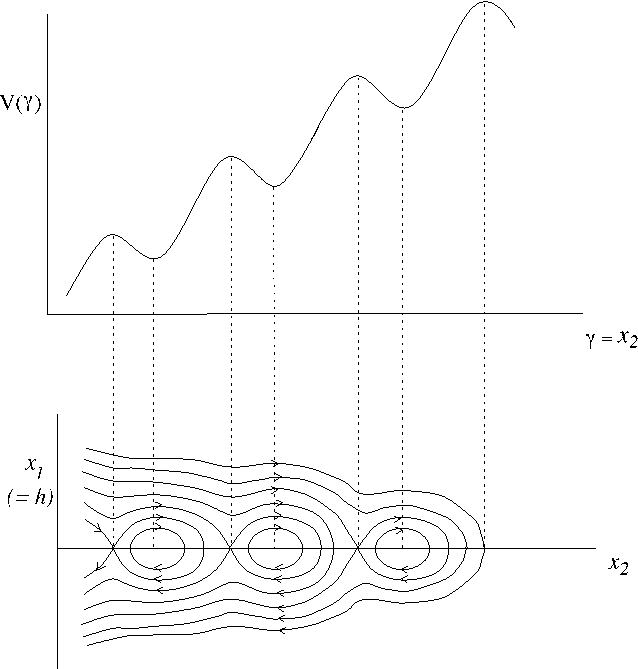
\includegraphics[width=\textwidth*2/3]{figures/asme_portrait}
\end{center}
\caption{Phase portrait}
\label{F:phase2}
\end{figure}
\begin{figure}
\begin{center}
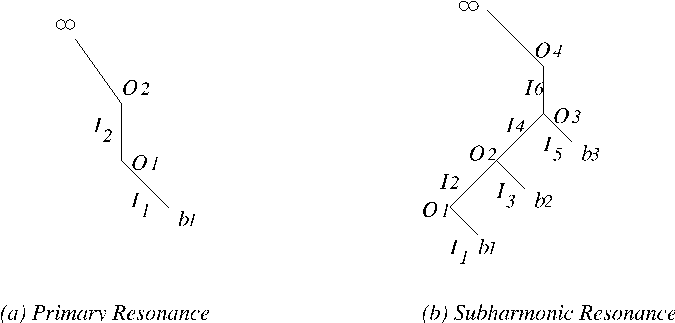
\includegraphics[width=\textwidth]{figures/reducespace}
\end{center}
\caption{Reduced space $\Graph$}
\label{F:reducespace}
\end{figure}

First, the unperturbed averaged Hamiltonian system~\eqref{e:flow} for $m = n = 1$ (i.e., primary resonance) has three fixed points: a center, $b_1$, and two saddles, $\Order_1, \Order_2$ along the $x_2$ ($=\gamma$)-axis. Here the reduced state space is $\Graph = \bigcup_{i=1}^2 \Int_i \bigcup b_1 \bigcup_{i=0}^2 [\Order_i]$, where
\begin{align*}
\Int_1 &\equiv \cup_{\substack{ x=(x_1,x_2) \in \bar \Ss\\
H(x) < \Order_1\\
x \ne b_1}} [x],& \Int_2 &\equiv \cup_{\substack{ x=(x_1,x_2) \in \bar \Ss\\
{\Order}_1<H(x)<{\Order}_2 }} [x],&
\Int_3 &\equiv \cup_{\substack{ x=(x_1,x_2) \in \bar \Ss\\
H(x)>{\Order}_2}}[x].
\end{align*}
See Figure~\ref{F:reducespace}(a). Secondly, the Hamiltonian system~\eqref{e:flow} for $m=3,\ n=1$ (i.e., sub-harmonic resonance) has seven fixed points: three centers, $b_{1,2,3}$, and four saddles, $\Order_{1,2,3,4}$ along the $x_2$-axis. Here the reduced state space is, as illustrated in Figure~\ref{F:reducespace}(b), $\Graph = \bigcup_{i=1}^7 \Int_i \bigcup_{i=1}^3 b_i \bigcup_{i=1}^4 [\Order_i]$, where
\begin{align*}
\Int_1 &\equiv \cup_{\substack{x=(x_1,x_2) \in \bar \Ss\\
H(x)<{\Order}_1\\
x \ne b_1}} [x], & \Int_2 &\equiv \cup_{\substack{ x=(x_1,x_2) \in \bar \Ss\\
{\Order}_1< H(x) < \Order_2\\
x_2 < \{x_2: x = \Order_2 \}}} [x], & \Int_3 &\equiv \cup_{\substack{x=(x_1,x_2) \in \bar \Ss\\
H(x)<{\Order}_2\\
x \ne b_2\\
x_2 > \{x_2: x = \Order_4\}}} [x]\\
\Int_4 &\equiv \cup_{\substack{ x=(x_1,x_2) \in \bar \Ss\\
\Order_2 < H(x) < \Order_3\\
x_2 < \{x_2:x = \Order_3\}}} [x], & \Int_5 &\equiv \cup_{\substack{ x = (x_1,x_2) \in \bar \Ss\\
H(x)<{\Order}_2\\
x \ne b_3\\
x_2 > \{x_2:x = \Order_3\}}} [x], & \Int_6 &\equiv \cup_{\substack{x = (x_1,x_2) \in \bar \Ss\\
{\Order}_3<H(x) < \Order_4}} [x]\\
& &
\Int_7 &\equiv \cup_{\substack{ x=(x_1,x_2) \in \bar \Ss \\
H(x)>{\Order}_4}} [x]
\end{align*}
It should be noted that the Hamiltonian system is $2m\pi$ periodic in the angle variable $x_2$. Namely, the potential for the primary resonance (1:1) contains a single well while the potential for the sub-harmonics (3:1) contains three wells. Besides, except for the orbits inside the closed homoclinic orbits, the remnant of orbits have open trajectories, i.e., their periods become infinite. Henceforth, we can no longer carry out the averaging in the path integrals, namely, the integration with respect to the \emph{Hausdorff measure} in Definition~\ref{D:AVE}. The time averaged drift and diffusion coefficients on each leg $\Int_i$ are calculated as
\begin{align*}
\Tave & (\gen H -(b^1, \nabla K)) =\frac{2m \Omega^\prime (I^{m:n}) \mu_1^2 \left[(1 - k^2) K(k) + (2k^2-1)E(k)\right]}{3\pi n \Omega(I^{m:n}) (1-2k^2)^{3/2}}\\
& - m \Omega^\prime(I^{m:n}) \zeta h^2 \left[(1 - 2k^2)^2 E^2(k)-2(1-3k^2+2k^4)E(k)K(k)+ \right.\\
& \left.(1-5k^2+4k^4)K^2(k) \right]/ \left[3k^2(k^2-1)K^2(k)\right]\\
& + m \Omega^\prime(I^{m:n}) \mu_0 (1 - 2k^2)^2 \pi\ \omega\ \sech^2 A h^2 \sin \gamma \times\\
& \left[-2\cosh A K(k) \left\{(1-2k^2)E(k)+(k^2-1)K(k)\right\} + \right.\\
& \left. \sinh A (2k^2-1)m \pi \left\{ E(1 - k^2)K(k)+(E(k)-K(k))K(1 - k^2)\right\} \right]/\\
& \left[4 \sqrt{2} k^2 \sqrt{1 - 2k^2}(k^2 - 1)K^3(k)\right]\\
& + \frac{m}{4 \pi} (\zeta J_1 -\mu_0 J_2 \Omega^{''}(I^{m:n}) h^2 \sin \gamma)
+ \frac{m}{2 \pi} (\zeta J_1 -\mu_0 J_2 \sin\gamma) \zeta{\mathcal E}_1\\
& +\frac{ (\zeta J_1 -\mu_0 J_2 \sin \gamma)}{2 \pi} \mu_0 (1 - 2k^2)^2 \pi \omega \sech^2 A \cos \gamma \times\\
& \left[- 2\cosh A K(k) \left\{(1-2k^2)E(k)+(k^2-1)K(k)\right\} + \right.\\
& \left. \sinh A (2k^2-1) m \pi \left\{ E(1 - k^2) K(k) + (E(k) - K(k)) K(1 - k^2)\right\} \right]/\\
&\left[ 4\sqrt{2} \ k^2\sqrt{1-2k^2}(k^2-1)K^3(k)\right]
+ \frac{m}{2\pi} \Omega'(I^{m:n})(\zeta J_1-\mu_0 J_2 \sin \gamma) \mathcal E_2,\\
\Tave &(\langle dH, dH \rangle) = \frac{4 m^2 {\Omega'} ^2(I^{m:n}) 
\mu_1^2 h^2 \left[(1-k^2) K(k)+(2k^2-1)E(k)\right]}{3\pi
n\Omega(I^{m:n}) (1-2k^2)^{3/2}}
\end{align*}
where
\begin{gather*}
\begin{aligned}
A &= \frac{m \pi K(1 - k^2)}{2K(k)}, & \mathcal E_1 &= \frac{\omega}{2\pi m}\left.\int_0^{2\pi m/\omega} \frac{\partial x}{\partial I} y \ dt \right|_{I=I^{m:n}},
\end{aligned}\\
{\mathcal E}_2 = \frac{\omega}{2\pi m} \int_0^{2\pi m/\omega}
u_1 ds.
\end{gather*}
Here the modulus $k$ is determined by the resonant orbit $I^{m:n}$ and the detailed calculation of time averaging above are available in \citet[Appendix F]{choi03:_dynam}.

\begin{figure}
\begin{center}
\psfrag{h}{$H$}
\psfrag{b}{$\mathring b$}
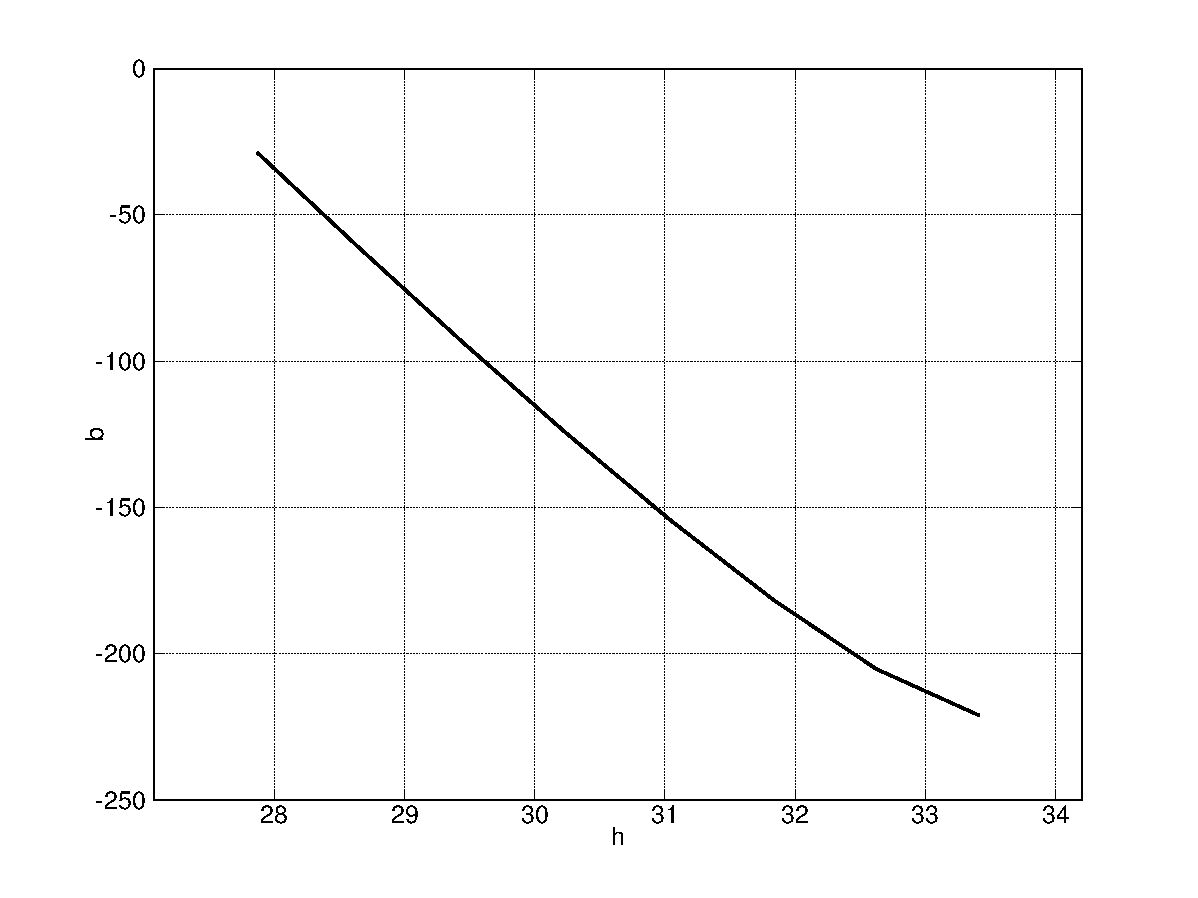
\includegraphics[width=\textwidth*7/8]{figures/oscillator_drift}
\caption{Drift coefficient, $\mathring b$, as a function of the Hamiltonian, $H$.}
\label{f:drift}
\end{center}
\end{figure}

\begin{figure}
\begin{center}
\psfrag{h}{$H$}
\psfrag{s}{$\mathring \sigma$}
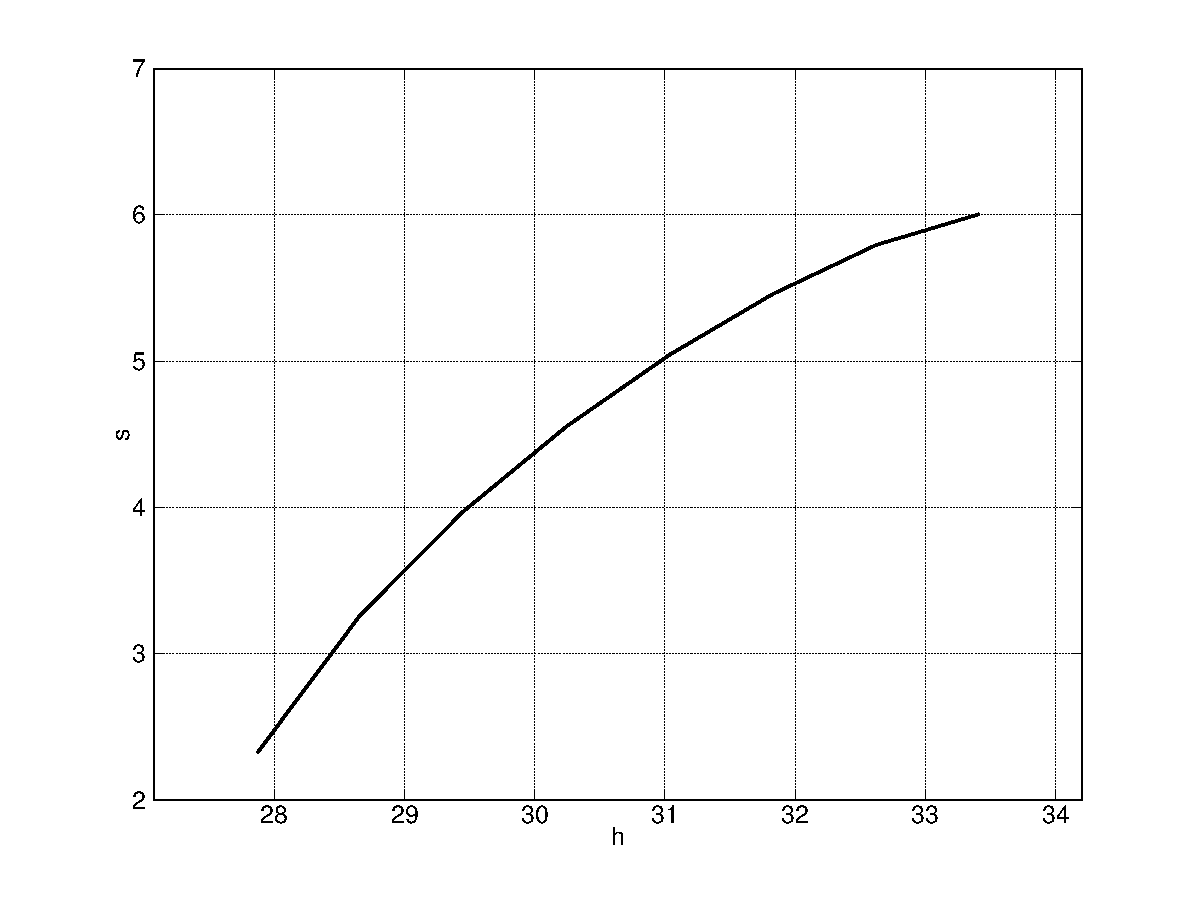
\includegraphics[width=\textwidth*7/8]{figures/oscillator_diffusion}
\caption{Diffusion coefficient, $\mathring \sigma$, as a function of the Hamiltonian, $H$.}
\label{f:diffusion}
\end{center}
\end{figure}

\section{Stationary Probability Density}
\label{S:stationary pdf}

In this section, we examine the stationary probability density of random motions in the resonance zone. The stationary probability density is obtained by solving the Fokker--Planck equation, namely,
\begin{equation}
\gen_i^{adj}\ p_i(z)=-\frac{1}{\period_i}J_i'(z_i) =0, \quad z \in \Int_i,
\label{e:FPE}
\end{equation}
where the probability current which is constant in each leg $\Int_i$ is defined
\[
J_i(z) \equiv \mathring b_i(z) p_i(z)- \frac12
\left({\mathring \sigma}^2_i(z) p_i(z)\right)', \quad z \in
\Int_i,
\]
where the definitions of $\mathring b$ and $\mathring \sigma$ follow Equations \eqref{e:oscillator drift} and \eqref{e:oscillator diffusion}, but the $\Aave$ averaging operator is applied without division by the period.

The limiting domain for our case is
\begin{multline*}
\dom^{adj} = \{p\in C(\Graph)\cap C^2(\cup_{i=1}^N\Int_i):
\text{$\lim_{h \to h_s}(\gen^{adj}_i p_i)(h)$ exists $\forall
i$,}\\
\sum (\pm)J_i(h_s)=0, \text{ and } J_i(\crit_i)=0 \},
\label{E:dom-adjoint}
\end{multline*}
At each of the centers, the so called \emph{entrance boundary} is prescribed because the drift coefficient at the centers is positive whereas the diffusion coefficient is equal to zero. Physically speaking, an entrance boundary (or reflecting boundary) cannot be reached from the interior of the state space because the positive sign of the drift pushes towards the inside. Thus, there is zero net flow of probability across the boundary, which implies that the probability current (or flux) in each leg $\Int_i$ which contains a center becomes identically zero. The reader is referred to \citet{karlin81:_secon_cours_stoch_proces} for a detailed discussion regarding the classification of boundaries. Further, the conservation of probability flux at the interior vertices is imposed

The solution of~\eqref{e:FPE} for the energy level sets is obtained as
\begin{multline*}
p_i(h) = \frac{1}{{\mathring{\sigma}}^2_i(h)}\exp
\left\{2\int^h_{h_i^\crit} \frac{\mathring{b}_i(\eta)}{{\mathring{\sigma}}^2_i(\eta)}\ d\eta \right\} \times\\
\left[ C_i \int^h_{h_i^\crit} \exp \left\{-2
\int^\eta_{h_i^\crit}\frac{\mathring{b}_i(\xi)}{{\mathring{\sigma}}^2_i(\xi)}\
d\xi \right\}\ d\eta +D_i \right] .
\end{multline*}
We need to determine unknown constants $C_i$ and $D_i$ from the prescribed conditions. First, $C_i$'s become identically zero due to the fact of zero probability current condition in the legs $\Int_i$'s which include the centers in Fig.~\ref{F:reducespace}. On the other hand, we have the same constant probability current in the rest of legs due to the conservation of probability current at the interior vertices. We specify the conditions necessary to solve the unknown constants for the primary and sub-harmonic resonance, respectively. For the primary resonance ($1:1$) we encounter $3$ unknown constants, i.e., $D_1,\ C_2,\ D_2$. Then in order to determine them, we apply one continuity and one periodic boundary condition at the saddles
\[
p_1(\Order_1)=p_2(\Order_1)=p_2(\Order_2)
\]
normalization. For the sub-harmonic resonance case ($3:1$), we have
$9$ unknowns, i.e., $D_1,\ C_2,\ D_2,\ D_3,\ C_4,\ D_4,\ D_5,\
C_6,\ D_6$. Thus, in order to determine them completely, we need
nine conditions. Firstly, we apply five continuity conditions and
one periodic boundary condition at the saddle points
\begin{align*}
p_1(\Order_1) &= p_2(\Order_1)=p_6(\Order_4)\\
p_2(\Order_2) &= p_3(\Order_2)=p_4(\Order_2)\\
p_4(\Order_3) &= p_5(\Order_3)=p_6(\Order_3).
\end{align*}
Secondly, we have the conserved probability current at each of saddle points which leads to
\[
C_2 = C_4 = C_6,
\]
and the normalization,
\[
\sum_{i=1}^N \int_{z\in \Int_i} p_i(z)\ dz = 1
\]
completes the determination of the constants.

Graphical results are given in Figures~\ref{reson_den1} and \ref{reson_den2}. For the primary resonance case, we have set the driving frequency $\omega=2$, the damping coefficient $\zeta=1$, the amplitude of the periodic force $\mu_0 = (R^m + 5) \zeta$, and the ratio $R^m(\omega)=3.97$. The corresponding resonant orbit which is determined by the resonance condition becomes $I^{1:1}=0.6345$ in terms of the elliptic modulus. In a similar manner, for the sub-harmonic resonance case, we carried out the numerical analysis with the following values: $\omega=4$, $\zeta=1$, $\mu_0 = (R^m + 20) \zeta$, $R^m(\omega)=23.8$, and $I^{3:1}=0.5068$ (graphical results are omitted.)
\begin{figure}[htbp]
\begin{center}
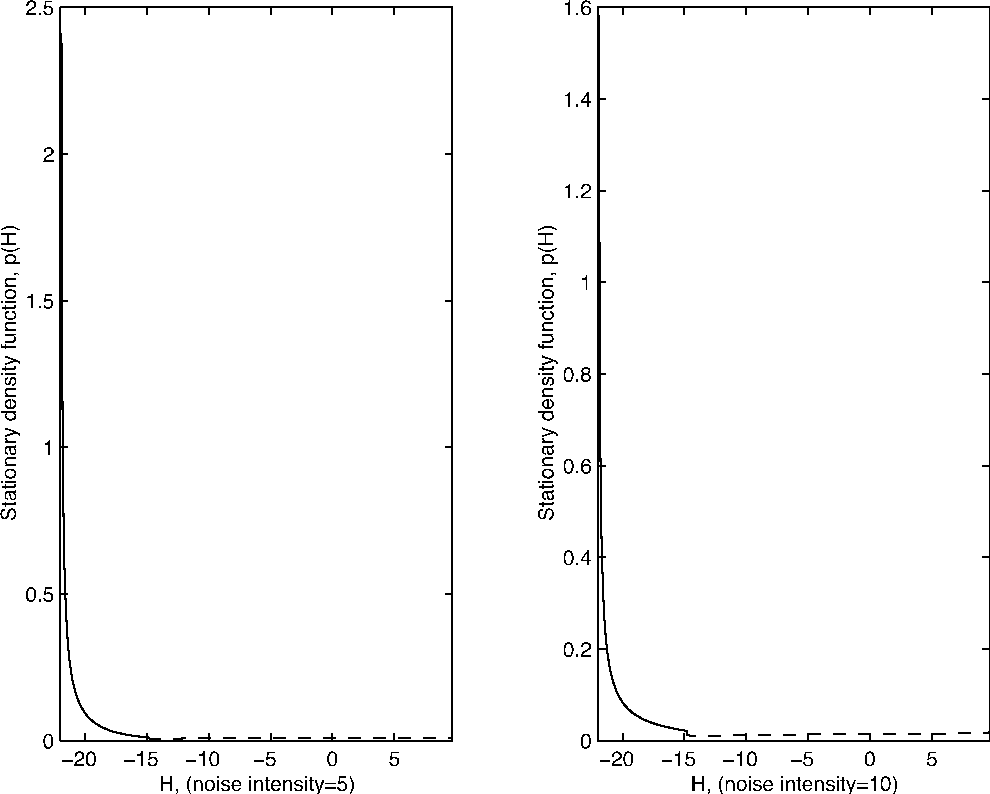
\includegraphics[width=\textwidth]{figures/res_den1}
\caption{Stationary probability density at $1:1$ resonance}
\label{reson_den1}
\end{center}
\end{figure}
\begin{figure}[htbp]
\begin{center}
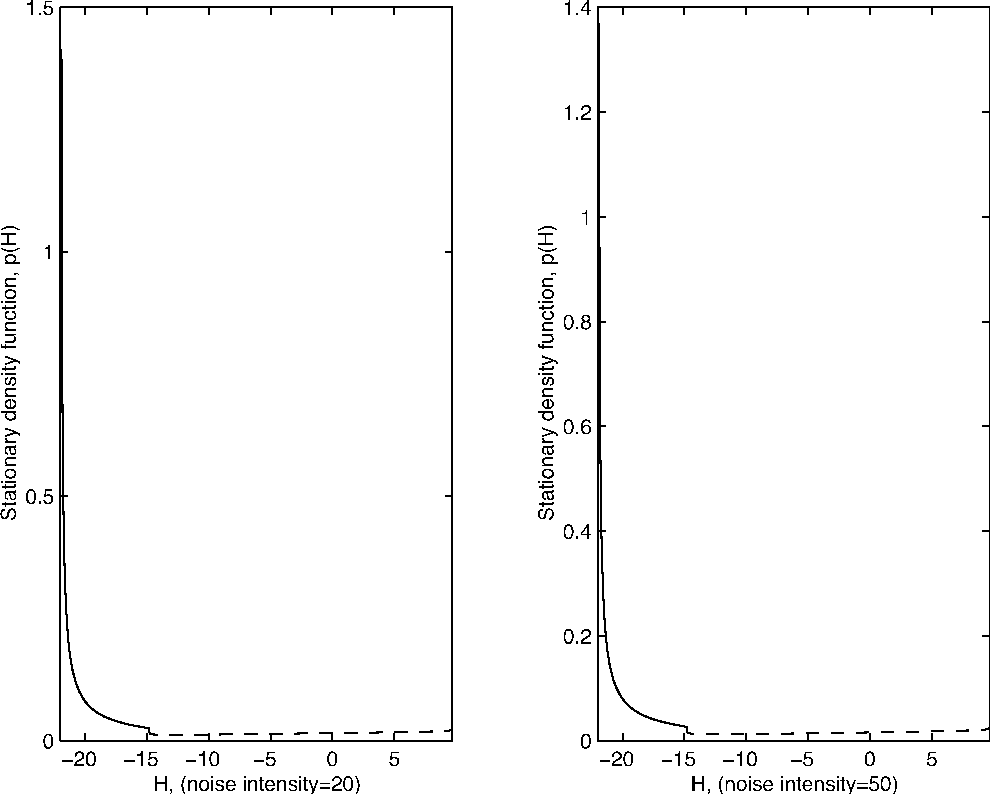
\includegraphics[width=\textwidth]{figures/res_den2}
\caption{Stationary probability density at $1:1$ resonance}
\label{reson_den2}
\end{center}
\end{figure}

\section{Validation With Sample Path Method}

To validate the solutions to the Fokker--Planck equation shown in Figures~\ref{reson_den1} and \ref{reson_den2}, a numerical procedure inspired by the heterogeneous multi-scale methods for stochastic differential equations \citep{e05:_analy} is developed. Instead of solving the FPE, the underlying stochastic differential equations are solved directly.

The stochastic differential equation to be solved is
\begin{equation}
dz = \mathring b(z) dt + \mathring \sigma(z) dW_t,\label{e:hmm sde}
\end{equation}
with $\mathring b$ and $\mathring \sigma$ defined by Equations \eqref{e:oscillator drift} and \eqref{e:oscillator diffusion}. Our numerical validation is used is a multiscale method in the sense that $\Aave$-averaging is performed numerically with time-averaging and the stochastic differential equation above is solved on a longer timescale. At each time-step of the ``macroscopic'' SDE, microscopic $\Aave$-based time averaging is performed.

First, the period of Hamiltonian orbits over which $\Aave$ averaging occurs must be determined. We do this using numerical integration and in that procedure, polar coordinates are used with the arc length being parametrized by the angle variable, $\theta$.

Rewriting the Hamiltonian given in Equation \eqref{E:hamiltonian-ave} as
\[
H = a_1 h^2 + a_2 \gamma + a_3 \cos(\gamma)
\]
where
\begin{align*}
a_1 &= \frac{m}{2} \frac{\partial \Omega}{\partial I} (I^{m:n}), &
a_2 &= \frac{\zeta}{2\pi} J_1, &
a_3 &= \frac{\mu_0}{2\pi} J_2.
\end{align*}
The orbits are translated by $y_c$ so their center is at the origin:
\[
\tilde y = y - y_c,
\]
and polar coordinates are introduced
\begin{align*}
x &= r \cos \theta, &
\tilde y &= r \sin \theta.
\end{align*}
Thus Equation \eqref{E:hamiltonian-ave} becomes
\begin{equation}
H = a_1 (r \cos \theta)^2 + a_2 (r \sin \theta + y_c) + a_3 \cos(r \sin \theta + y_c).
\label{e:hamiltonian polar}
\end{equation}
The arc length formula is
\[
\int_{\theta_1}^{\theta_2} \sqrt{\left(\frac{dr}{d\theta}\right)^2 + r^2} d\theta
\]
Using Equation \eqref{e:hamiltonian polar}, $r(\theta)$ is found numerically (in Octave, the function \emph{fsolve} is used) and to find $dr/d\theta$ one uses
\[
\frac{dr}{d\theta} = \frac{\partial f/\partial \theta}{\partial f/\partial r},
\]
where
\begin{gather*}
\partial f/\partial \theta = -2 a_1 r^2 \cos \theta \sin \theta + a_2 r \cos \theta - a_3 \sin(r \sin \theta + y_c) r \cos \theta,\\
\partial f/\partial r = 2 a_1 r \cos^2 \theta + a_2 \sin \theta - a_3 \sin(r \sin \theta + y_c) \sin \theta.
\end{gather*}
The period is found by numerical quadrature (in Octave, the function \emph{quad} is used.) Thus
\[
T = 2 \int_0^\pi \sqrt{\left(\frac{dr}{d\theta}\right)^2 + r^2} d\theta.
\]

Equation \eqref{e:hmm sde} is solved numerically using the Euler-Maruyama first order scheme \citep{kloeden92:_numer_solut_stoch_differ_equat}
\[
z_{n+1} = z_n + b_n \Delta t + \sigma_n \Xi_{n+1} \sqrt{\Delta t},
\]
where $\Xi_n$ are normally distributed random numbers with mean zero and variance one. Illustrative results obtained with the drift and diffusion coefficients in Figures \ref{f:drift} and \ref{f:diffusion} are shown in Figure \ref{f:sample pdf}.

\begin{figure}
\begin{center}
\psfrag{H}{$H$}
\psfrag{p}{$p$}
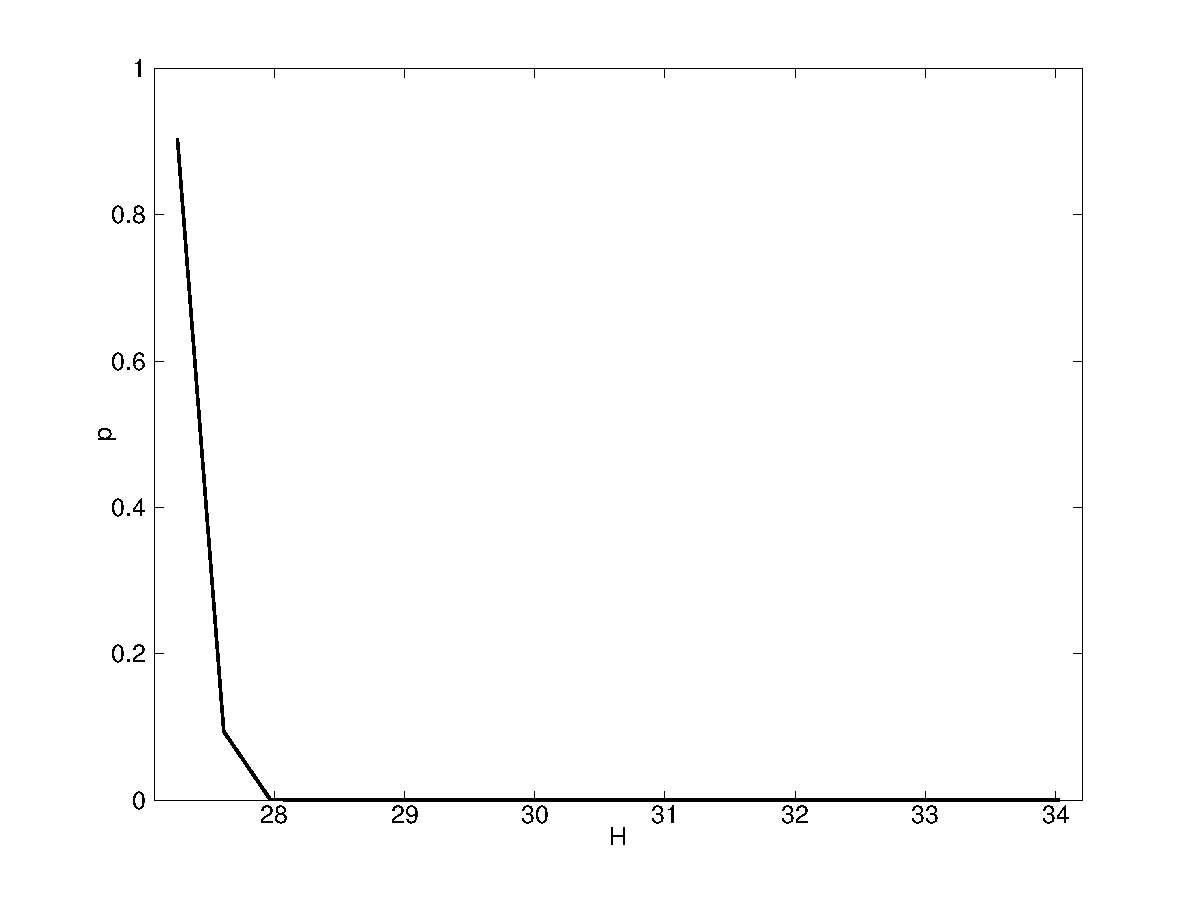
\includegraphics[width=\textwidth*7/8]{figures/oscillator_steady_state_pdf}
\caption{Steady state PDF as a function of the Hamiltonian, $H$. The PDF is produced with the sample path method. 3444 samples have been used. The time-step was set to $10^{-2}$ and 20 time-steps were taken.}
\label{f:sample pdf}
\end{center}
\end{figure}

\section{Conclusions}

An averaging approach has been developed to explore the near resonant motion of a noisy, strongly nonlinear periodically forced system. We first rewrote the perturbed Hamiltonian system with strong nonlinearity in action space by means of a canonical transformation. We introduced local coordinates adjacent to the resonance surface and performed the appropriate rescaling which allows us to see the correct asymptotics. After stochastic averaging, the resulting reduced model became a graph valued process under capture into resonance. Since we addressed a separation of time scales, such a methodology enabled us to diminish the dimension of the original model. The reduced process converged in probability to a Markov process as $\tilde\epsilon \to 0$. The associated limiting generator has furnished statistical quantities such as the probability density function. The effects of noisy perturbations were investigated through such a statistical description.

Some investigators, including \citet{soskin89:_fluct, soskin92:_evolut}, have shown there is no dramatic stochastic resonance phenomenon in a system whose oscillation frequency is a monotonically increasing function of energy (see Fig.~\ref{F:frequency}(a).) In systems with \emph{asymmetric} single-well potentials with a non-monotonic frequency variation (see Fig.~\ref{F:frequency}(b)), however, dramatic stochastic resonance has been shown to emerge at optimal noise. Thus, in view of our analysis, we conjecture that the existence of P-bifurcations in asymmetric systems may be connected to stochastic resonance.


\chapter{Surface Gravity Waves}
\label{c:sgwaves}
\section{Introduction}

Surface waves form at the free surface of a liquid. For additionally clarity, they are sometimes called surface gravity waves. This emphasizes that gravity (and not, for example, surface tension) is the dominant restoring force.

Surface waves have captured the interest of many scientists. Michael Faraday was among them and he was sufficiently successful to have a problem in surface wave motion named after him. In 1831, Faraday reported to the Royal Society \citep{faraday31:_acous_figur} on experiments he did in which a thin layer of water was placed on a vibrating membrane. Faraday established that the standing waves that form on the plate have an oscillation frequency equal to one-half the vertical forcing frequency used to produce them. It is due to this discovery that nowadays, many investigations in wave excitation are known under the rubric of the `Faraday problem.'

% % Faraday's result established 1:2 ratio with external forcing, to
% % produce 1:1 internal resonance, is horizontal forcing required, or
% % is vertical forcing also acceptable? Check paper given by NSN on
% % canonical transformation

In certain applications, for example in experiments carried out on spacecraft where `g-jitter' is hard to eliminate \citep{walter87:_fluid}, there is a need to describe the surface gravity wave patterns that form under the influence of `noisy' forcing. Thus, in the present development we focus on stochastic forcing. Specifically, we examine the long-term evolution of a horizontally excited Faraday system when two wave-modes are near 1:1 resonance and show that in this case, rather than studying the fast timescale evolution of two individual wave modes (i.e. a four-dimensional system), one can focus on the long timescale evolution of two conserved quantities (the Hamiltonian and the angular momentum.)

\section{Surface-Gravity Wave Model}
\subsection{Governing Equations}
\label{s:governing equations}

Although our ultimate goal is to study surface wave patterns, we begin by considering the `internal' motion of the fluid at whose surface these wave patterns form. For an incompressible fluid whose velocity is described by the vector $\boldsymbol{u}$, the Boussinesq approximation~\citep{kundu90:_fluid_mechan} holds and conservation of mass is expressed by the continuity equation
\begin{equation}
\nabla \cdot \boldsymbol{u}= 0 \label{e:Cons Mass}
\end{equation}
For a fluid particle with density $\rho$, pressure $p$ and viscosity $\nu$ (and with gravity represented by the vector $\boldsymbol{g}$), conservation of momentum is expressed by the equation
\begin{equation}
\rho \left[ \frac{\partial \boldsymbol{u}}{\partial t} + (\boldsymbol{u} \cdot \nabla )\boldsymbol{u} \right] = - \nabla p + \rho \boldsymbol{g}+ \nu \nabla^2 \boldsymbol{u}. 
\end{equation}
This equation is known by many as the Navier-Stokes equation. We are working towards a Hamiltonian formulation, therefore we assume the fluid is invscid and the Navier-Stokes equation simplifies to the Euler equation
\begin{equation}
\rho \left[ \frac{\partial \boldsymbol{u}}{\partial t} + (\boldsymbol{u} \cdot \nabla )\boldsymbol{u} \right] = - \nabla p + \rho \boldsymbol{g}.
\end{equation}
Note, however, that we will reintroduce viscous effects (in \S\ref{s:damping}) in the form of linear damping.

Next, the fluid motion is assumed irrotational: $\nabla \times \boldsymbol{u}= 0$. This assumption can either be introduced ad-hoc, or it can be inferred from Kelvin's circulation theorem. The latter states that for inviscid fluids, rotational motion is conserved. Therefore, if we take the initial state of the fluid to be irrotational, it will remain irrotational forever after. Irrotational fluid motions can be described by a velocity potential $\boldsymbol{u}= \nabla \phi$. The conservation of momentum equation becomes
\begin{equation}
\frac{\partial \phi}{\partial t} + \frac12 |\boldsymbol{u}|^2 + \frac{p}{\rho} + g z = 0.
\end{equation}
In the above, it has been assumed gravity acts along the vertical direction, therefore $|\boldsymbol{g}|=g$.

In order to relate the motion of the surface waves to the internal motion of the fluid, boundary conditions are needed. First, there is the kinematic boundary condition. As explained in \citet{whitham74:_linear}, derivation of this boundary condition, the kinematic boundary condition is based on the surface of the fluid being defined by the property that no fluid crosses it. This surface has height
\begin{equation}
z = \eta (x_1, x_2, t)
\end{equation}
($x_1$ and $x_2$ refer to the coordinates of the horizontal plane, in actual calculations we use cylindrical coordinates, thus $x_1 = r$ and $x_2 = \theta$) and the kinematic boundary condition is given by
\begin{equation}
\frac{\partial \eta}{\partial t} + \nabla \eta \cdot \boldsymbol{u} = u_z \quad \text{at } z = \eta
\end{equation}
In the above, we have made use of the notation $\boldsymbol{u} = (u_{x_1}, u_{x_2}, u_z )$. The second condition at the free surface is known as the dynamic boundary condition. It reflects the fact that pressure changes continuously across the interface. The dynamic boundary condition is given by
\begin{equation}
\frac{\partial \phi}{\partial t} + \frac12 |\boldsymbol{u}|^2 + |\boldsymbol{g}|z = 0 \quad \text{at } z = \eta .
\end{equation}
In our treatment, we take the fluid to be confined to a cylindrical tank of radius $a$ and depth $d$ (at rest the fluid is contained between $z = -d$ and $z = 0$.) This leads to boundary conditions at the lateral and bottom walls of the tank that state that there is no flow across these walls
\begin{gather*}
u_r = 0 \quad \text{at } r = a\\
u_z = 0 \quad \text{at } z = - d
\end{gather*}

An essential contribution made by \citet{miles76:_nonlin} is to show that the conservation of mass equation, the kinematic boundary condition and the boundary conditions at the lateral and bottom walls can be obtained from a variational formulation. Specifically, the first variation of the integral
\begin{equation}
\begin{split}
SI (\phi)& = \int_{\theta = 0}^{2 \pi} \int_{r = 0}^a \int_{z = - d}^{\eta ( r, \theta, t )} \frac12 | \nabla \phi |^2 dz \, dS - \int_{\theta = 0}^{2 \pi} \int_{r = 0}^a  \phi |_{z = \eta} \frac{\partial \eta}{\partial t} dS
\end{split}
\end{equation}
must vanish ($S = \pi r^2$ is the cross-sectional area of the basin). Miles's derivation was based on work by \citet{serrin59:_encyc_physic}. Note that Miles's derivation is different from the oft-cited variational in \citet{luke67:_variat_princ_for_fluid_with_free_surfac} since the latter also recovers the dynamic boundary condition. Note furthermore that a similar variational analysis was obtained earlier by \citet{zakharov68:_stabil_of_period_waves}.

First, separation of variables is used to write
\begin{align*}
\eta (x_1,x_2, t)& = q_n (t) \psi_n (x_1,x_2),\\
\phi (x_1,x_2,z,t)& = \phi_n (t) \chi_n (x_1,x_2,z).
\end{align*}
The relationship between $\psi_n$ and $\chi_n$ is found from the conservation of mass equation, the boundary condition at the container's walls and a linearization of the kinematic boundary condition
\begin{equation}
\frac{\partial \eta}{\partial t} = \frac{\partial \phi}{\partial z} \quad \text{at } z = 0.
\end{equation}
The relation between $\phi_n(t)$ and $q_n(t)$ is found using the variational formulation. Details are given in~\citet[\S2]{miles76:_nonlin}.

% Give specific form of eigenfunctions, and eigenvalues for
% cylindrical geometry

% Show sample diagram of surface wave pattern

\subsection{The Hamiltonian of Surface-Gravity Waves}
\label{s:Hamiltonian}

Stochastic averaging may be seen as a procedure used to reduce the number of dimensions of a system. The lower-dimensional system's long-term evolution is given in terms of quantities that are constants of motion of the original (higher dimension) system over short timespan. This motivates our interest in determining the Hamiltonian for the surface-gravity wave system. First, we write expressions for the kinetic and potential energies. These give the Lagrangian from which the Hamiltonian follows.

The kinetic energy is
\begin{eqnarray*}
T & = & \frac12 \int | \nabla \phi |^2 dS dz\\
& = & \frac{\rho S}{2} a_{mn} \dot{q}_m \dot{q}_n .
\end{eqnarray*}
The second form of $T$ makes use of the results in~\citet{miles76:_nonlin}, where it is shown that
\begin{equation}
a_{mn} = \delta_{mn} a_m + a_{lmn} q_l + \frac12 a_{jlmn} q_j q_l + O ( q^2 )
\end{equation}
The quantities $a_{lmn}$ and $a_{jlmn}$ are constants. The potential energy of the free-surface, displaced from its equilibrium position, is
\begin{eqnarray}
V & = & \rho \int dS \int^{\eta}_{z = 0} |\boldsymbol{g}| z dz \label{e:potential energy}\\
& = & \frac{\rho S}{2} g q_n q_n. \nonumber
\end{eqnarray}
The Lagrangian, which for convenience we normalize by $\rho S$, is
\begin{eqnarray*}
L & = & \frac{1}{\rho S} ( T - V )\\
& = & \frac12 ( a_{mn} \dot{q}_m \dot{q}_n - g q_n q_n ) .
\end{eqnarray*}
and the Hamiltonian is
\begin{equation}
\label{e:Hamiltonian}
H = \frac12 (h_{mn}(q) p_m p_n + g q_n q_n).
\end{equation}
Note that this Hamiltonian contains quadratic terms, but also higher order terms since the coefficient $h_{mn}$ depends on $q_n$
\begin{equation}
\label{e:hamiltonian coefficient expansion}
h_{mn} = \delta_{mn} \frac{\omega_m^2}{g} + h_{lmn} q_l + \frac12 h_{jlmn} q_j q_l + O(q^3).
\end{equation}
The equations for $h_{lmn}$ and $h_{jlmn}$ are given in \citet{miles76:_nonlin} and reproduced in Appendix~\ref{a:non-linear Hamiltonian}

\subsection{Damping and Forcing Effects}
\label{s:damping}

We are interested in the effects of stochastic forcing. To balance forcing effects, damping is necessary. Physically, damping stems from the viscosity of the fluid, but for simplicity we introduce damping ad-hoc. We use linear damping coefficients, $\alpha_k$ to supplement the momentum equation.
% FIXME This approach is also used by Miles in \cite{miles84:_inter}, however Miles also supplements the equations for $q_1$ and $q_2$ with damping, but it is not clear how to physically justify the damping of coordinates.

To account for forcing effects, we follow the method presented in~\citet{miles76:_nonlin}. Terms are added to the potential energy given in Equation (\ref{e:potential energy}), thus
% FIXME Should not have to give multiple references to miles76:_nonlin
\begin{equation}
\begin{split}
V &= \rho \int dS \int^{\eta}_{z = 0} \bigl[ \dot{\xi}_{x_1}
x_1 + \dot{\xi}_{x_2} x_2 + (g + \dot{\xi}_z) z \bigr] dz\\
&= \rho S \bigl( - Q_n q_n + \frac12 (g + \dot{\xi}_z) q_n q_n
\bigr)\label{e:V with forcing}.
\end{split}
\end{equation}
In the above $\xi_{x_1}$ and $\xi_{x_2}$ specify the imposed horizontal velocities of the tank while $\xi_z$ is the vertical velocity and
\begin{align}
Q_n & = - \dot{\xi}_{x_1} x_{1 n} - \dot{\xi}_{x_2} x_{2
n}\\ x_{1 n} & \equiv S^{- 1} \int x_1 \psi_n dS\label{e:SI def}\\ x_{2 n} &
\equiv S^{- 1} \int x_2 \psi_n dS
\end{align}
With forcing and damping, the equations governing the motion of the
surface-gravity waves are, for $t\geq0$,
\begin{align}
\dot{q}_k &= \frac{\partial H}{\partial p_k}\\
\dot{p}_k &= -\frac{\partial H}{\partial q_k} + \alpha_k p_k +
\dot{\xi}_z q_1 + \dot{\xi}_{x_1} x_{1k} + \dot{\xi}_{x_2} x_{2k}
\end{align}

\section{Stochastic Analysis}
In this section, we analyze the equations of motion presented in the
previous section under the influence of stochastic
forcing. Specifically, we concentrate on the motion of two wave modes
near resonance.

\subsection{Integrals of Motion}\label{s:Integrals of motion} In
order to study the effects of small amplitude noise over long time
scales, we introduce a small scaling parameter $\epsilon$
($0<\epsilon\ll1$.) First, we rescale the canonical variables by
$\sqrt{\epsilon}$
\begin{align*}
q &=\sqrt{\epsilon}\tilde{q}& 
p &=\sqrt{\epsilon}\tilde{p}.
\end{align*}
Concentrating our analysis on the two wave modes (near resonance), we use the canonical transformation
\begin{gather*}
\tilde{q}_{1,2} = x_{1,2} \cos \omega_{1,2} t +\tfrac{\omega_{1,2}}{g} y_{1,2} \sin
\omega_{1,2} t\\
\tilde{p}_{1,2} = -\tfrac{g}{\omega_{1,2}} x_{1,2} \sin \omega_{1,2} t + y_{1,2} \cos
\omega_{1,2} t
\end{gather*}
% FIXME \omega vs. omega_{1,2} and \epsilon
This transformation eliminates terms of order $\epsilon$ in the
Hamiltonian. The lowest order terms of the Hamiltonian are now of
order $\epsilon^{3/2}$. Terms of that order are eliminated by
setting the two wave modes near resonance with one another, so that
$\omega_{1,2} = \omega + \epsilon \sigma_{1,2}$. This imposition and the time averaging operator from Definition \ref{d:Tave} eliminate terms of order $\epsilon^{3/2}$ from the Hamiltonian. Thus the dynamics of the system acquire the form
\begin{align}
\dot{\boldsymbol{x}}^{\epsilon}_t& = \epsilon \boldsymbol{b}^1
(\boldsymbol{x}^{\epsilon}_t,t) + \epsilon^2 \boldsymbol{b}^2
(\boldsymbol{x}^{\epsilon}_t,t) + \epsilon \boldsymbol{g}
(\boldsymbol{x}^{\epsilon}_t,t)
\label{e:standard form}
\end{align}
% \begin{equation}
% \boldsymbol{b}^1 \equiv \frac{1}{\epsilon^2} \bar{\nabla} H, \quad
% \bar{\nabla} \equiv
% \Bigl(
% \frac{\partial}{\partial y_1}, 
% -\frac{\partial}{\partial x_1},
% \frac{\partial}{\partial y_2},
% -\frac{\partial}{\partial x_2}
% \Bigr)
% \end{equation}
% is of order 1 in $\epsilon$ and corresponds to the `Hamiltonian
% dynamics' term in the equation
% \begin{align}
% \dot{\boldsymbol{x}}^{\epsilon}_t& = \epsilon \boldsymbol{b}^1
% (\boldsymbol{x}^{\epsilon}_t,t) + \epsilon^2 \boldsymbol{b}^2
% (\boldsymbol{x}^{\epsilon}_t,t) + \epsilon \boldsymbol{g}
% (\boldsymbol{x}^{\epsilon}_t,t), & t \geq 0 \label{e:standard form}\\
% \boldsymbol{x}_0^\epsilon& = \boldsymbol{x}\nonumber \in \R^4
% \end{align}
% $\boldsymbol{b}^2$ refers to damping terms
% \begin{align*}
% \boldsymbol{b}^2 \equiv
% \Bigl(&
% \frac{\omega}{g} \alpha_1  \left[ -\frac{g}{\omega} x_1 \sin
% \omega t + y_1 \cos \omega t \right] \sin \omega t
% ,\\&
% \alpha_1 [-\frac{g}{\omega} x_1 \sin \omega t + y_1 \cos
% \omega t] \cos \omega t
% ,\\&
% \frac{\omega}{g} \alpha_2  \left[-\frac{g}{\omega} x_2
% \sin \omega t + y_2 \cos \omega t \right] \sin \omega t
% ,\\&
%  \alpha_2 [ - \frac{g}{\omega} x_2 \sin \omega t + y_2 \cos
% \omega t] \cos \omega t
% \Bigr)
% \end{align*}
% $\boldsymbol{g}$ contains stochastic forcing terms. Note that because
% vertical forcing is parametric whereas horizontal forcing is additive,
% if one were interested in a problem with both types of forcing
% present, the horizontal forcing would need to be smaller than the
% vertical forcing by a factor of $\sqrt{\epsilon}$, as can be seen from
% Equation~\eqref{e:V with forcing}. We avoid this complication by
% considering only horizontal forcing.
% \begin{align*}\label{e:g def}
% \boldsymbol{g} \equiv
% \Bigl(&
% \frac{\omega}{g} \Bigl[ \dot{\xi}_z \Bigl( x_1 \cos \omega t +
% \frac{\omega}{g} y_1 \sin \omega t \Bigr) + \dot{\xi}_{x_1} x_{11}
% + \dot{\xi}_{x_2} x_{21} \Bigr]  \sin \omega t
% ,\\ &
% \frac{\omega}{g} \Bigl[\dot{\xi}_z \Bigl( x_1 \cos \omega t +
% \frac{\omega}{g} y_1 \sin \omega t \Bigr) + \dot{\xi}_{x_1} x_{11}
%  + \dot{\xi}_{x_2} x_{21} \Bigr] \cos \omega t
% ,\\ &
% \frac{\omega}{g}  \Bigl[ \dot{\xi}_z \Bigl( x_2 \cos \omega t +
% \frac{\omega}{g} y_2 \sin \omega t \Bigr) + \dot{\xi}_{x_1} x_{12}
%  + \dot{\xi}_{x_2} x_{22} \Bigr] \sin \omega t
% ,\\ &
% \frac{\omega}{g} \Bigl[
% \dot{\xi}_z \Bigl( x_2 \cos \omega t + \frac{\omega}{g} y_2 \sin \omega t
% \Bigr) + \dot{\xi}_{x_1} x_{12} 
%  + \dot{\xi}_{x_2} x_{22} \Bigr] \cos \omega t
% \Bigr)
% \end{align*}
Equation~\eqref{e:standard form} is helpful in showing
the three timescales present in this problem. Owing to their small
amplitude (i.e. $\epsilon^2$), the effects of noise and damping have an
influence only over long times, of order $1/\epsilon^2$. The
Hamiltonian dynamics, associated with the components of
$\boldsymbol{b}^1$ are of order $\epsilon$, thus they fluctuate over a
faster timescale, of order $1/\epsilon$. Finally, the fastest
fluctuations occur due periodicity of some of the coefficients that
constitute $\boldsymbol{b}^1$. The coefficients fluctuate over a
period $\omega/2\pi$, which is of order 1. % Our interest is primarily
% in the influence of stochastic forcing, thus we must use two averaging
% steps, the first to average the periodic coefficients and the second
% to average the dynamics of $\boldsymbol{b}^1$. This type of stochastic
% averaging was developed in Namachchivaya and
% Sowers~\cite{namachchivaya01:_unified_approac_noisy_nonlin_mathieu_type_system}
% for a two-dimensional system. Here we apply the method to a
% four-dimensional system, following the extensions presented
% in~\cite{namachchivaya:_random}.

% In order for a four-dimensional system to be integrable, two integrals
% of motion are needed. To find these constants, we begin by defining
% our first averaging operator. For a function $\varphi$ that is
% time-periodic with period $\omega/2 \pi$
% \begin{equation}
% \Tave\varphi \equiv \frac{\omega}{2\pi}
% \int_0^{2\tfrac{\pi}{\omega}} \varphi(t) dt
% \label{e:time averaging defn}
% \end{equation}
% This is a deterministic averaging operator. Applying this
% operator to the periodic coefficients (those that fluctuate over
% timescales of order 1) eliminates them, so that the fastest timescale
% of the problem is now of order $1/\epsilon$.
We rescale time such that leading order dynamics become of order
1. If $\tilde{\boldsymbol{x}}_t^{\epsilon} \equiv
\boldsymbol{x}_{t/\epsilon}^{\epsilon}$. Equation~\eqref{e:standard
form} becomes
\begin{align*}
\dot{\tilde{\boldsymbol{x}}}^{\epsilon}_t& = \boldsymbol{b}^1
({\tilde{\boldsymbol{x}}}^{\epsilon}_t,t/\epsilon) + \epsilon
\boldsymbol{b}^2
({\tilde{\boldsymbol{x}}}^{\epsilon}_t,t/\epsilon) +
\boldsymbol{g} (\tilde{\boldsymbol{x}}^{\epsilon}_t,t/\epsilon)
\end{align*}
% \begin{align*}
% \dot{\tilde{\boldsymbol{x}}}^{\epsilon}_t& = \boldsymbol{b}^1
% ({\tilde{\boldsymbol{x}}}^{\epsilon}_t,t/\epsilon) + \epsilon
% \boldsymbol{b}^2
% ({\tilde{\boldsymbol{x}}}^{\epsilon}_t,t/\epsilon) +
% \boldsymbol{g} (\tilde{\boldsymbol{x}}^{\epsilon}_t,t/\epsilon), & t
% &\geq 0\\
% \tilde{\boldsymbol{x}}_0^\epsilon& = \boldsymbol{x} \in \R^4
% \end{align*}
With the equation in this form, we are able to apply a result from~\citet{khas'minskii66:_stoch_proc}. This result tells us that as $\epsilon \to 0$, $\tilde{\boldsymbol{x}}_t^\epsilon$ converges in probability to
\begin{align*}
\dot{\boldsymbol{x}}_t &= \Tave[\boldsymbol{b}^1(\boldsymbol{x}_t,t/\epsilon)] = \bar{\nabla}\Tave[H(\boldsymbol{x}_t)] = \bar{\nabla} K(\boldsymbol{x}_t), & t \geq 0\\
\boldsymbol{x}_0 &= \boldsymbol x \in \Real^4
\end{align*}
The averaged Hamiltonian, $K$, is our first integral of motion.
\begin{multline*}
K =\frac{1}{192 g^3 \omega}\bigl[3 k^2 K_1 (y_1^2+y_2^2)^2
\omega^5 + 3g^4 (32(\sigma_1 x_1^2 + \sigma_2 x_2^2)+k^2 K_1 \omega
(x_1^2+x_2^2)^2)\\
+ 2g^2 \omega^2 \{48(\sigma_1 y_1^2 + \sigma_2 y_2^2) + k^2 (32 K_{-1}
(x_2 y_1-x_1 y_2)^2+K_1[(3 x_1^2+x_2^2) y_1^2 \\
+ 4 x_1 x_2 y_1 y_2 + (x_1^2 + 3 x_2^2) y_2^2])\omega\}\bigr]
\end{multline*}

% In Mathematica file, K = H - O(2) terms

% In order to find the second integral of motion, we take advantage of
% the fact we are interested in 1:1 resonance by writing
% $\omega_1=\omega + \epsilon \sigma_1$ and $\omega_2=\omega + \epsilon
% \sigma_2$. This introduces `detuning', of order $\epsilon$ into the
% problem. Note that we have the freedom to choose the order of the
% detuning; detuning of order $\epsilon$ is chosen so that detuning is
% of the same order as the Hamiltonian terms that do not vanish under
% time-averaging. Detuning could be made of higher-order, in which case
% its effects would presumably be chosen to be of the same order as
% stochastic forcing and damping. Setting $\omega_1$ and $\omega_2$ as
% stated provides a second integral of motion:

The second integral of motion will be denoted by $I$ and represents
angular momentum.
\begin{equation}
I= \frac{1}{2 g \omega}\bigl[g^2(x_1^2+x_2^2)+\omega^2(y_1^2+y_2^2)\bigr].
\end{equation}

\subsection{Structure of the Unperturbed System}
\label{s:unperturbed structure}

As stated in the previous section, the surface wave system in 1:1 resonance has two constants of motion, $K$ and $I$. We now introduce a canonical transformation that takes advantage of this fact by making the angular momentum one of the canonical variables. The canonical transformation from $(x_1,y_1,x_2,y_2)$ to $(X,Y,\theta,I)$ is given by
\begin{align*}
x_1& = \frac{\sqrt{\frac{\omega}{g}(X^2+Y^2)}}{Y \sqrt{1+\frac{X^2}{Y^2}}} (Y \cos \theta - X \sin \theta)\\
y_1& = -\frac{\sqrt{\frac{g}{\omega}(X^2+Y^2)}}{Y \sqrt{1+\frac{X^2}{Y^2}}} (X \cos \theta + Y \sin \theta)\\
x_2& = \sqrt{\frac{\omega}{g} (2I-X^2-Y^2)} \cos \theta\\
y_2& = -\sqrt{\frac{g}{\omega} (2I-X^2-Y^2)} \sin \theta.
\end{align*}
Introducing the variables
\begin{align*}
\alpha &\equiv \frac{k^2 \omega^2}{24 g}(K_1 - 16 K_{-1}) & \beta 
&\equiv \frac{3 k^2 \omega^2}{24 g} K_1
\end{align*}
the averaged Hamiltonian is
\begin{equation}
\label{e:averaged K}
K = \frac{\alpha}{2} (X^2 + Y^2 - 2 I) X^2 + \frac{\beta}{2} I^2 + \frac{\sigma_1 - \sigma_2}{2}(X^2 + Y^2) + \sigma_2 I
\end{equation}
and the equations of motion are
\begin{equation}
\label{e:sgwaves fast planar}
\begin{gathered}
\dot{X}_t = (\alpha X_t^2 + \sigma_1 - \sigma_2) Y_t\\
\dot{Y}_t = [\alpha(2I_t - 2X_t^2 - Y_t^2) - \sigma_1 + \sigma_2] X_t\\
\dot I_t = 0\\
\dot \theta_t = \beta I_t - \alpha X_t^2 + \sigma_2
\end{gathered}
\end{equation}
% FIXME Add order epsilon terms to these equations
This canonical transformation decouples the equations
for $X_t$ and $Y_t$ from those for $\theta_t$, and, consistent with
the results of \S\ref{s:Integrals of motion}, $I_t$ is a
constant (effectively a parameter) since $\dot{I}_t=0$. $I$ acts as a
bifurcation parameter. Defining the critical value
\begin{equation}
I_c = \frac{\sigma_1 - \sigma_2}{2 \alpha},
\end{equation}
when $I<I_c$ phase portraits in the $X,Y$ plane have a single elliptic
fixed point at the origin. For $I>I_c$, the fixed point at the origin
becomes a saddle point and two fixed points on the $X$ axis
appear. The coordinates of these fixed points are
\begin{align}
X &= \pm \sqrt{I + \frac{\sigma_2 - \sigma_1}{2 \alpha}} &
Y = 0
\end{align}

% This is depicted in Figure~\ref{f:bifurcation and phase portrait}.

The stochastic diffusion process that we will study is described in terms of the variables $K$ and $I$. The $K-I$ domain is shown in figure~\ref{f:HI domain}. In that figure, $I$ ranges from 0 to 0.5, but the upper limit can be made arbitrarily large. The range of $K$ is not arbitrary. The maximum value, $K_e$ occurs at the elliptic fixed points. There is also a minimum value, $K_{2I}$, since the canonical transformation introduces the restriction $X^2 + Y^2 \leq 2 I$. Note that the domain between $K_s$ and $K_e$ exits for both elliptic fixed points, thus, the entire $K-I$ domain may be described as a three-leaved open-book, a nomenclature used in~\citet{freidlin04:_diffus}, or an arrowhead.

% FIXME State that a cusp exists in the domain.

% \begin{figure}
% \begin{center}
% \includegraphics[width=\textwidth*5/8,angle=-90]{../../matlab/figures/phaseportrait_xy_3d_subcrit}
% \caption{Phase-space portrait in the $X,Y$ plane when $I < I_c$}
% \label{f:X Y phase portrait I < I_c}
% \end{center}
% \end{figure}

% \begin{figure}
% \begin{center}
% \includegraphics[width=\textwidth]{../../matlab/figures/phaseportrait_xy_3d_supcrit}
% \caption{Phase-space portrait in the $X,Y$ plane when $I > I_c$}
% \label{f:X Y phase portrait}
% \end{center}
% \end{figure}

% FIXME Produce and insert figure below
% \begin{figure}
% \begin{center}
% \includegraphics[width=\textwidth]{figures/bifurcation_and_phase_portrait}
% \caption{Phase-space portrait and bifurcation diagram}
% \label{f:bifurcation and phase portrait}
% \end{center}
% \end{figure}

\begin{figure}
\begin{center}
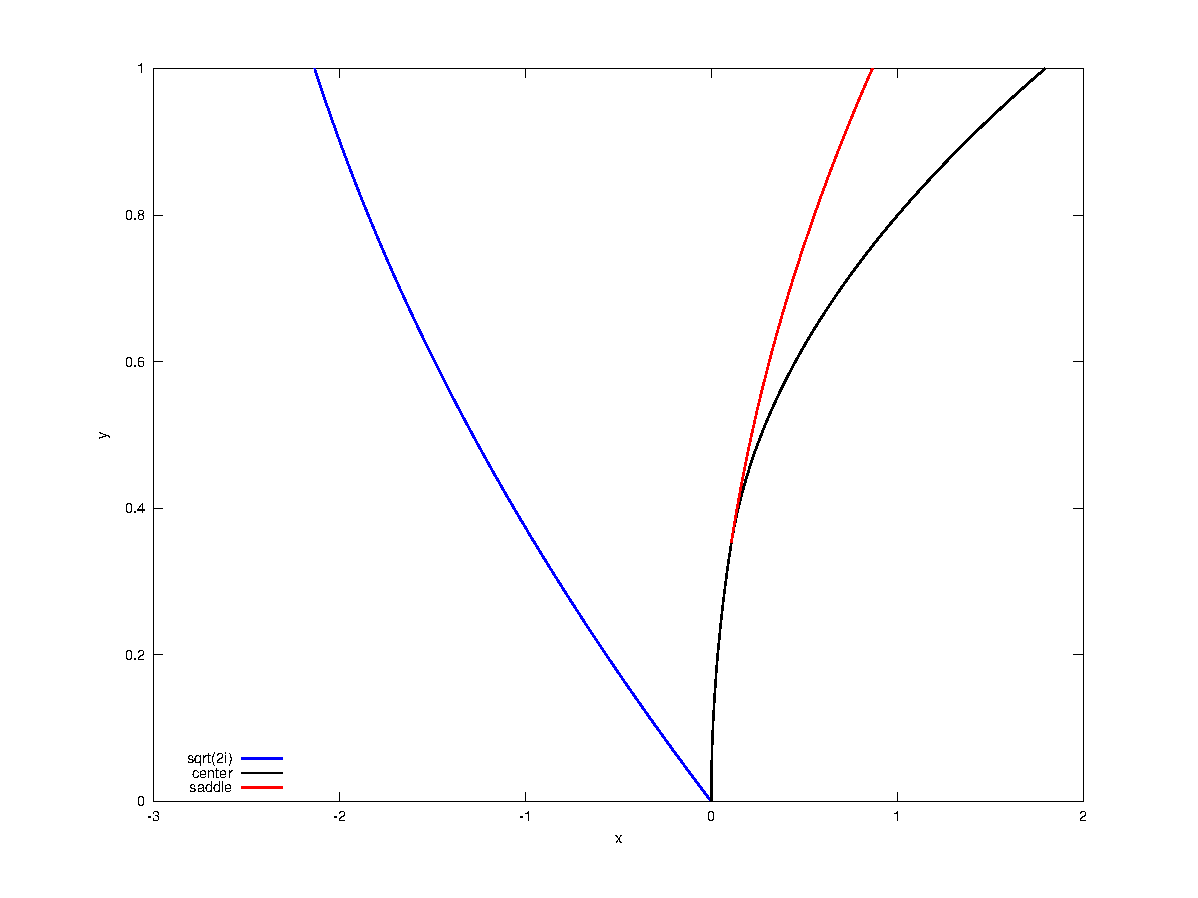
\includegraphics[width=\textwidth*7/8,angle=0]{figures/HIdomain}
\caption{$K-I$ domain}
\label{f:HI domain}
\end{center}
\end{figure}
% FIXME Add FEM triangulation to this figure

% \subsection{Evolution of the Integrals of Motion}

% The ultimate goal of our analysis is to understand the effects of noise. The amplitude of the noise being small, its effects are seen only over long times. The effect of noise (and damping) is seen in the evolution of the two conserved quantities, $K$ and $I$. It seems natural therefore, to define the map $\mathcal{Y}: \Real^4 \to \Real^2$ by
% \begin{equation}
% \mathcal{Y}(\boldsymbol{x}) \equiv (K(\boldsymbol{x}),I(\boldsymbol{x})), \qquad \boldsymbol{x}\in \Real^4.
% \end{equation}
% Since $\lim_{\epsilon \to 0}\boldsymbol{x}^\epsilon_t =
% \boldsymbol{x}_t$,
% % Need to quote Khasminksii here?
% \begin{equation}
% \lim_{\epsilon \to 0}(K(\boldsymbol{x}^\epsilon_t),I(\boldsymbol{x}^\epsilon_t)) = (K(\boldsymbol{x}_t),I(\boldsymbol{x}_t)).
% \end{equation}
% The evolution of $\boldsymbol{y}^{\epsilon}_t \equiv \mathcal{Y}(\boldsymbol{x}^{\epsilon}_t )$ is given by
% \begin{align}
% \dot{\boldsymbol{y}}^{\epsilon}_t& = \epsilon F^1(\boldsymbol{x}^{\epsilon}_t,t) + \epsilon^2 F^2(\boldsymbol{x}^{\epsilon}_t,t) + \epsilon G
% (\boldsymbol{x}^{\epsilon}_t,t), & t& \geq 0 \label{e:SDE}\\
% \boldsymbol{y}_0^\epsilon& = (K(\boldsymbol{x}),I(\boldsymbol{x}))
% \end{align}
% where
% \begin{align*}
% F^1_1& = \sum^4_{i = 1} \frac{\partial K}{\partial\boldsymbol{x}_i} \boldsymbol{b}^1_i&
% F^1_2& = \sum^4_{i = 1} \frac{\partial I}{\partial\boldsymbol{x}_i} \boldsymbol{b}^1_i\\
% F^2_1& = \sum^4_{i = 1} \frac{\partial K}{\partial\boldsymbol{x}_i} \boldsymbol{b}^2_i&
% F^2_2& = \sum^4_{i = 1} \frac{\partial I}{\partial\boldsymbol{x}_i} \boldsymbol{b}^2_i\\
% G_1& = \sum^4_{i = 1} \frac{\partial K}{\partial\boldsymbol{x}_i} \boldsymbol{g}_i&
% G_2& = \sum^4_{i = 1} \frac{\partial I}{\partial \boldsymbol{x}_i} \boldsymbol{g}_i
% \end{align*}
% Since $K$ and $I$ are integrals of motion, $\Tave F^1 (\boldsymbol{x}) = 0$. Thus, to see the fluctuations of $K$ and $I$, we need to look on an a timescales of order $1/\epsilon^2$. Thus, we rescale time again, setting $\boldsymbol{X}^{\epsilon}_t \equiv \boldsymbol{x}^{\epsilon}_{t / \epsilon^2}$ and $\boldsymbol{Y}_t^{\epsilon} \equiv \boldsymbol{y}^{\epsilon}_{t / \epsilon^2}$. This yields
% \begin{align}
% \dot{\boldsymbol{X}}^{\epsilon}_t& = \frac{1}{\epsilon} b^1 (
% \boldsymbol{X}^{\epsilon}_t, t/\epsilon^2) + b^2
% (\boldsymbol{X}^{\epsilon}_t,t/\epsilon^2) + \frac{1}{\epsilon}
% g(\boldsymbol{X}^{\epsilon}_t,t/\epsilon^2), & \label{e:X}
% t&\geq 0\\
% \boldsymbol{X}^\epsilon_0& = \boldsymbol{x} \in \Real^4 \nonumber
% \end{align}
% \begin{align}
% \dot{\boldsymbol{Y}}^{\epsilon}_t& = \frac{1}{\epsilon} F^1
% (\boldsymbol{X}^{\epsilon}_t,t/\epsilon^2) + F^2
% (\boldsymbol{X}^{\epsilon}_t,t/\epsilon^2) + \frac{1}{\epsilon}
% G(\boldsymbol{X}^{\epsilon}_t,t/\epsilon^2), & \label{e:Y}
% t& \geq 0\\
% \boldsymbol{Y}_0^\epsilon& =
% (K(\boldsymbol{x}),I(\boldsymbol{x})) \nonumber
% \end{align}
% FIXME Show that as \eps \to 0, evolution of slow variables becomes independent of fast variables. 

% \subsection{Martingale Problem}

% In order to carry out our stochastic analysis, we must rigorously characterize the dynamics of Equation~\eqref{e:Y}. The classical analysis of such equations dates back to Khas'minksii. As shown in \S\ref{s:unperturbed structure}, the reduced domain (i.e. $K \times I$) of the surface wave equations contains a saddle fixed point. For such a case, as opposed to a domain free of fixed points in its interior, showing that $Y_t^\epsilon$ is a Markov process (where it must be stressed that by this we mean $Y_t^\epsilon$ alone, without being coupled to the $X_t^\epsilon$ equations) has only been done via the martingale problem approach.

% To introduce the martingale problem, let us consider the process $X_t^\epsilon$ rather than $Y_t^\epsilon$. The martingale problem is stated in terms of a canonical process $X_t$. This canonical process is made of deterministic parts (the Hamiltonian dynamics and the damping in our case) and stochastic parts (forcing.) The stochastic part has a probility measure $\mathbbm{P}^o$ and this is also the `induced' probability for $X_t^\epsilon$. $X_t$ on the other hand has a probability measure $\mathbbm{P}^\epsilon$ and the correspondence between the two probability measure is given, in terms of a set $A$, as
% \begin{equation}
% \mathbbm{P}^\epsilon(A) \equiv \mathbbm{P}\{X^\epsilon \in A\}
% \end{equation}
% (this transfers the dependence on $\epsilon$ from the process to the
% measure.)

% The martingale problem states that the measure $\mathbbm{P}^\epsilon$
% is unique and that it has a martingale associated with it. A
% martingale, $M_s$ is a process for which
% \begin{equation}
% \Expectation[M_s | \mathcal{M}_t] = M_t \quad\text{for all }s \ge t.
% \end{equation}
% $\mathcal{M}_t,t\ge 0$ is a filtration.

% The process $Y_t^\epsilon$ `lives' in a reduced 2-D space. Denoting
% the reduced-space canonical process corresponding to $Y_t^\epsilon$ by
% $X_t^\dagger$ and the probability measure of $X_t^\dagger$ by
% \begin{equation}
% \mathbbm{P}^{\epsilon,\dagger}(A) \equiv \mathbbm{P}^\epsilon(Y \in A)
% \quad A \in \mathcal{B}(C[0,\infty),K\times I),
% \end{equation}
% the novel requirements for the class of problems within which the
% stochastic analysis of the surface waves falls is to show the
% existence of the limit
% \begin{equation}
% \mathbbm{P}^\dagger \equiv \lim_{\epsilon \to 0}
% \mathbbm{P}^{\epsilon,\dagger}
% \end{equation}
% % We do not show this proof here (it is in preparation by~\citet{namachchivaya:_random}.) Here we simply emphasize that in order to treat a domain $K \times I$ with fixed points, the Martingale problem approach is required and using this approach, classical results are augmented with gluing conditions.

% \subsection{Generator of the Reduced Markov Process}
% \label{s:MP generator}

% In the previous section, we stated the existence of a reduced process $X_t^\dagger$ with a probability measure $\mathbbm{P}^\dagger$. In this section, we give detailed results characterizing the Markov process.

% Let's denote by $\mathfrak{G} = K \times I$ the space shown in figure~\ref{f:HI domain}. To begin, we decompose $\mathfrak{G}$ into three disjoint regions: one for each of the two regions enclosed by a homoclinic orbit and the third outside the homoclinic orbit.

% %As $\epsilon \to 0$, the dynamics of
% %$\boldsymbol{Y}^{\epsilon}_t$ tend to a two-dimensional Markov
% %process~\cite{NamachchivayaUnpublished}. We turn our attention to
% %finding the generator of this Markov process.

% %For $I<I_c$, the stochastic process evolves in a 2-dimensional
% %plane. In this case, the stochastic averaging results
% %in~\cite{khas'minskii68:_ito} hold, making the our analysis relatively
% %straightforward. As shown in Figure~\ref{f:HI domain},
% %$K$ ranges from its value at $X^2 + Y^2 = 2 I$, which we
% %denote by $K_{2I}$ to its value at the elliptic fixed
% %points, $K_e$ and $I$ ranges from 0 to $I_c$. We denote the
% %space of the averaged system by

% %\begin{equation}
% %\mathfrak{G}=([K_{2I},K_e],[0,I_c])=([\boldsymbol{y}_*,\boldsymbol{y}^*]).
% %\]

% %The generator is
% %% What is the limit y' -> y ? Closure of spaces...
% %\begin{equation}\label{e:generator line process}
% %\begin{split}
% %(\gen_\mathfrak{G}^\dagger f)(\boldsymbol{y})& = \lim_{\boldsymbol{y}'
% %\to \boldsymbol{y}, \boldsymbol{y} \in \mathfrak{G}} (\gen f) (\boldsymbol{y}')\\
% %& = \mathfrak{b}_j(\boldsymbol{y}) \frac{\partial
% %f(\boldsymbol{y})}{\partial \boldsymbol{y}_j} + \frac12
% %\mathfrak{a}_{jk}(\boldsymbol{y}) \frac{\partial^2
% %f(\boldsymbol{y})}{\partial \boldsymbol{y}_j \partial \boldsymbol{y}_k}
% %\end{split}
% %\end{equation}
% %and the domain of the generator is
% %% What BC to apply at I_c boundary?
% %\begin{equation*}
% %\mathfrak{D}_\mathfrak{G}^\dagger = \{f \in C^2(\mathfrak{G}): \lim_{\boldsymbol{y}
% %\to (K_{2I},I)} (\gen f)(\boldsymbol{y}) \text{ exists, }
% %\lim_{\boldsymbol{y}
% %\to (K_e,I)} (\gen f)(\boldsymbol{y}) \text{ exists }
% %\text{ and }\\
% % \lim_{\boldsymbol{y} \to (K,I_c)}(\genf)(\boldsymbol{y})=0\}
% %\end{equation*}
% %The drift coefficient $\mathfrak{b}_i$ and diffusion coefficient
% %$\mathfrak{a}_{ij}$ will be defined shortly (viz. Equations~\eqref{eq:
% %drift coeff} and~\eqref{e:diff coeff}.)

% %When $I>I_c$, the analysis is slightly more involved. To begin, the
% %space $\mathfrak{G}$ is decomposed into three disjoint regions, one
% %inside each of the two homoclinic orbits and the third outside the
% %homoclinic orbits. Thus
% \begin{equation}
% \mathfrak{G} \equiv \bigcup_{i=1}^3 \bar{\mathcal{I}}_i.
% \end{equation}
% Within each $\bar{\mathcal{I}}_i$, we use classical results
% (e.g.~\citet{khas'minskii68:_ito}) to state that the generator of
% the reduced Markov process is, for a function $f \in
% C^2(\Real^2)$,
% \begin{equation} (\gen_{\mathcal{I}_i}^\dagger f)(\bm{y}) = \sum_{j=1}^2
% \mathfrak{b}^i_{y_j}(\bm{y}) \frac{\partial f(\bm{y})}{\partial y_j} +
% \frac12 \sum_{j,k = 1}^2 \mathfrak{a}^i_{y_j y_k}(\bm{y})
% \frac{\partial^2 f(\bm{y})}{\partial y_j \partial y_k}
% \end{equation}
% $\mathfrak{b}$ is the drift coefficient and $\mathfrak{a}$ the diffusion coefficient. In the present problem, because the equations of motion involve time-derivatives of noise, we apply a `real' noise with a specified spectral density rather than white noise (since the latter cannot be differentiated.) % Applying results from \citet{khas'minskii66:_limit_theor} yields the following
% % \begin{align}
% % \mathfrak{b}_{y_i} (\bm{y})& \equiv
% % (\mathbf{A}(\Tave(F^2_i +\mathfrak{g}_i))) (\bm{y})\label{e:drift coeff}\\
% % \mathfrak{a}_{y_j y_k} (\bm{y})& \equiv (\mathbf{A}(\Tave(\sigma\sigma^T)_{jk}))(\bm{y})\label{e:diff coeff}
% % \end{align}
% % where
% % \begin{align}
% % \mathfrak{g}_i& \equiv \int_{-\infty}^0 \Expectation\Bigl[\frac{\partial G_i}{\partial x_j}(\bm{x},t,\xi_t)G_j(\bm{x},t+\tau,\xi_{t+\tau})\Bigr] d\tau \label{e:script g}\\
% % (\sigma\sigma^T)_{jk}& \equiv \int_{-\infty}^\infty \Expectation \Bigl[G_j(\bm{x},t,\xi_t) G_k (\bm{x},t+\tau, \xi_{t+\tau}) \Bigr] d\tau \label{e:sigma sigmat}
% % \end{align}

Note that second order averaging terms have not been included because they may change our results quantitatively but not qualitatively. The small increase in the accuracy of our results is unlikely to be worth the extra effort due to significantly more complex algebraic manipulations.

% $\Aave$ is a spatial averaging operator. It is applied along orbits $S$ on which $K$ and $I$ are constant
% \begin{equation}
% \Aave(\varphi(\bm{y})) \equiv \frac{\int_S \varphi (\bm{y}) \| \bar{\nabla} K(\bm{y})\|^{-1} dS}{\int_S \| \bar{\nabla} K(\bm{y})\|^{-1} dS}.
% \label{e:A averaging}
% \end{equation}
% $\| \bar{\nabla} K(\bm{y})\|$ is a measure of speed,
% thus the denominator corresponds to a period, $\mathcal{T}$. At fixed
% points and on the homoclinic orbit, velocity is zero, thus the
% definition above does not hold. On the homoclinic orbit
% % What happens if linearize system about saddle point? Get inifinite period?
% $\lim_{K \to K_s}
% \mathcal{T}(K,I) \to \infty$ while at the elliptic
% fixed point $\mathcal{T}(K_e,I)$ the period is finite and
% equal to the period of the system linearized about the fixed
% point. At the saddle point, we will need to evaluate drift and
% diffusion coefficients without dividing by the (infinite) period. For
% notational convenience, we introduce
% \begin{equation}
% \begin{split}
% \mathring{\mathfrak{b}}_i& \equiv \mathfrak{b}_i \mathcal{T}\\
% \mathring{\mathfrak{a}}_{jk}& \equiv \mathfrak{a}_{jk} \mathcal{T}
% \end{split}
% \label{e:ring notation}
% \end{equation}

% Thus each $\mathcal{I}_i$ has a distinct generator
% $\gen_i$. The generators are linked along the edge
% $K_s$ by a `gluing' boundary condition. For a process that
% does not `stick' to any of the orbits, which is true for the surface
% waves, the gluing condition is
% \begin{equation}
% \sum_{i=1}^3 \{\pm\} \sum_{j=1}^2 \Bigl\{\sum_{k=1}^2
% \mathring{\mathfrak{a}}^i_{jk}(\mathcal{O})
% \frac{\partial f_i}{\partial y_k}\bigg|_{(\mathcal{O})}
% \Bigr\} \cdot \nu_j(\mathcal{O}) =0.
% \end{equation}
% The $+$ sign is taken if $K>K_s$ on the leg
% $\mathcal{I}_i$ and the $-$ sign is taken otherwise. $\nu_1$ and
% $\nu_2$ are unit vectors in the directions of $K$ and $I$
% respectively. $\mathcal{O}$ correspoinds to the line along which
% $K = K_s$.

% With the gluing condition specified, the domain of the generator of
% the process evolving on $\mathfrak{G}$ can be defined
% \begin{multline}
% \mathfrak{D}_\mathfrak{G}^\dagger = \{f \in C(\mathfrak{G}) \cap
% C^2(\bigcup_{i=1}^3 \mathcal{I}_i): \lim_{H \to
% K_{2I}} (\gen^\dagger_{I_3} f)(\bm{y}) \text{
% exists },\\
% \lim_{H \to K_c}(\gen^\dagger_{I_i} f)(\bm{y}) \text{ exists
% for } i = 1,2, \lim_{I \to I^*}
% \gen^\dagger_{I_i} = 0\; \forall\, i,\\
% \sum_{i=1}^3 \{\pm\} \sum_{j=1}^2 \Bigl\{\sum_{k=1}^2
% \mathring{\mathfrak{a}}^i_{jk}(\mathcal{O}) \frac{\partial f}{\partial
% y_k}\bigg|_\mathcal{O} \Bigr\} \cdot \nu_j(\mathcal{O}) =0 \}
% \label{e:generator domain}
% \end{multline}
% The first condition specifies behavior at the boundary
% where $X^2 + Y^2 = 2I$, the `outer' boundary. The limit as $H
% \to K_c$ specifies behavior at the two centre fixed
% points. The third condition holds in the limit $I^* \to \infty$.

% The open manifolds $\mathcal{I}_i$ do not include the fixed points
% (denoted by $c_i$) nor the homoclinic orbits whereas their closures
% $\bar{\mathcal{I}}_i$ do. Each $\mathcal{I}_i$ has a distinct
% generator $\gen_i$. The generators are linked at the
% saddle-point by a `gluing' boundary condition.

% The gluing condition depends solely on the diffusion coefficients
% $\mathfrak{a}^i_{jk}$~\cite{Freidlin1998}, thus we define
% \begin{equation}
% \hat{\mathfrak{a}}^i_{jk}(\boldsymbol{y}) = \mathfrak{a}^i_{jk}
% (\boldsymbol{y}) T (\boldsymbol{y}),
% \end{equation}
% with $T(\boldsymbol{y})$ representing the period of an orbit in
% phase-space. For a process that does not `stick' to any of the
% orbits, which is the case for the system under consideration, the
% gluing condition is

% We are now ready to rigorously define the generator
% \begin{equation}\label{e:generator graph process}
% \begin{split}
% (\gen^\dagger_\mathfrak{G} f)(\boldsymbol{y})& =
% \lim_{\boldsymbol{y}' \to \boldsymbol{y}, \boldsymbol{y} \in
% \mathcal{I}_i}(\gen_i f_i)(\boldsymbol{y}')\\
% & = \sum_{j=1}^2 \mathfrak{b}_j^i(\boldsymbol{y}) \frac{\partial
% f_i(\boldsymbol{y})}{\partial \boldsymbol{y}_j} + \frac12
% \sum_{j,k=1}^2 \mathfrak{a}_{jk}^i(\boldsymbol{y})\frac{\partial^2
% f_i(\boldsymbol{y})}{\partial \boldsymbol{y}_j \boldsymbol{y}_k}
% \end{split}
% \end{equation}
% and its domain
% \begin{multline}
% \mathfrak{D}_\mathfrak{G}^\dagger = \{f \in C(\mathfrak{G}) \cap
% C^2(\bigcup_{i=1}^3 \mathcal{I}_i):\lim_{\boldsymbol{y} \to
% \boldsymbol{y}(c_i)} (\gen_i f_i)(\boldsymbol{y})
% \text{ exists } \forall \hspace{0.25em} i, \lim_{\boldsymbol{y}_2 \to
% I^*}(\gen_i f_i)(\boldsymbol{y})=0 \hspace{0.25em} \forall
% \hspace{0.25em}i,\\
% \sum_{i=1}^3 \{\pm\} \sum_{j=1}^2 \Bigl\{\sum_{k=1}^2
% \hat{\mathfrak{a}}^i_{jk}(\mathcal{O}) \frac{\partial f_i}{\partial
% \boldsymbol{y}_k}\bigg|_\mathcal{O} \Bigr\} \cdot \nu_j(\mathcal{O})
% =0 \}\label{e:generator domain}
% \end{multline}

% FIXME Check 2-D gluing condition against result published by Freidlin

% Let us consider now the specific form of the drift and diffusion
% coefficients of the generator. Often in problems involving stochastic
% forcing, white noise is used as the forcing function. In the present
% problem, because the equations of motion involve time-derivatives of
% noise, we apply a `real' noise with a known spectral density
% instead. This is a mean-zero, stationary, independent stochastic
% process satisfying the strong mixing property, for which, as $\epsilon
% \to 0$, $\tfrac{1}{\epsilon}
% \xi(t/\epsilon^2)$ approaches a white noise process. Applying
% Khas'minskii's results~\cite{khas'minskii66:_limit_theor} yields the following

% \begin{align}
% \mathfrak{b}_i (\boldsymbol{y})& \equiv (\mathbf{A}(\Tave(F^2_i
% +\mathfrak{g}_i))) (\boldsymbol{y})\label{e:drift coeff}\\
% \mathfrak{a}_{jk} (\boldsymbol{y})& \equiv
% (\mathbf{A}(\Tave(\sigma\sigma^T)_{jk}))(\boldsymbol{y})
% \label{e:diff coeff}
% \end{align}
% where
% \begin{align*}
% \mathfrak{g}_i& \equiv \int_{-\infty}^0 \Expectation\Bigl[\frac{\partial
% G_i}{\partial
% x_j}(\boldsymbol{x},t,\xi_t)g_j(\boldsymbol{x},t+\tau,\xi_{t+\tau})\Bigr]
% d\tau
% \\
% (\sigma\sigma^T)_{jk}& \equiv \int_{-\infty}^\infty
% \Expectation \Bigl[G_j(\boldsymbol{x},t,\xi_t) G_k
% (\boldsymbol{x},t+\tau,
% \xi_{t+\tau}) \Bigr] d\tau
% \end{align*}
% and $\mathbf{A}$ is an averaging operator that we discuss
% below.
% Taking the expected value in the integrals above effectively
% introduces a correlation into our formulation, for example
% \begin{equation}
% \Expectation\left[\frac{d\xi_{x_1}}{dt}\bigg|_t
% \frac{d\xi_{x_2}}{dt}\bigg|_{t+\tau}\right] = R_{H_1 H_2}(\tau).
% \end{equation}
% Once this substition has been made, the definite integrals are
% evaluated using the Fourier 

% Note that Khas'minskii's definition of $\mathfrak{b}_i$
% includes an additional term known as the `second-averaging' term. We
% do not include this term here because it may change our results
% quantitatively but not qualitatively. The small increase in the
% accuracy of our results is unlikely to be worth the extra effort due
% to significantly more complex algebraic manipulations.

\subsection{Calculation of the Drift and Diffusion Coefficients}

The drift vector, $\mathfrak{b}$, and diffusion matrix, $\mathfrak{a}$, are defined by equations~\eqref{e:drift} and~\eqref{e:diffusion}. Up to and including the $\Tave$ averaging operator, calculations are carried out analytically. The final operation, $\Aave$ averaging is performed numerically.

The expectation operator used in Equations \eqref{e:drift} and \eqref{e:diffusion} leads to the introduction of correlation functions. For example
\begin{equation}
\Expectation[\dot{\xi}_{x_1}(t) \dot{\xi}_{x_2}(t+\tau)] = R_{H_1 H_2}(\tau).
\end{equation}
Furthermore, Fourier transforms are used, for example
\begin{equation}
\int_{-\infty}^0 R_{H_1 H_2} cos(\omega \tau) d \tau =
\sqrt{\frac{\pi}{2}} \mathcal{F}_c(\omega).
\end{equation}
% FIXME Ambiguous since H_1 H_2 not express by \mathcal{F}
Applying these two simplifications and setting $\xi_z = \xi_{x_2} = 0$, we obtain formulas for $\Tave(F_i^2 + \mathfrak{g}_i)$ and $\Tave(\sigma \sigma^T)_{jk}$ in terms of $X, Y$ and $I$. These formulas are given in Appendix~\ref{a:drift and diffusion coefficient integrands}.

The final step is $\Aave$-averaging. In Definition \ref{d:Aave}, this was presented as a time-averaging operation, but an equivalent definition can be given in terms of two-dimensional line integrals. For this, denote the $l^2$ norm by $\lVert\cdot\rVert$. Making use of the relationship between distance, velocity and time, the period of a Hamiltonian orbit, $S$, is then given by
\[
\period(y) = \int_S \lVert \bar \nabla K(x(s)) \rVert^{-1} ds.
\]
Using spatial integration the $Aave$-averaging operator in Definition \ref{d:Aave} can be rewritten
\[
(\Aave \varphi) (y) = \frac{1}{\period(y)} \int_S \varphi(x(s)) \lVert \bar \nabla K(x(s)) \rVert^{-1} ds.
\]

To make computations straightforward, Cartesian coordinates are parametrized by an angle variable, thus transforming 2-D line integrals into one dimensional integrals. This is helpful because it allows the use of standard one-dimensional numerical integrators to perform $\Aave$-averaging. This parametrization by $\theta$ is separated into two cases:
\begin{enumerate}
\item Orbits for which $I < I_c$ or $K_{2I} < K < K_s$. These orbits are centred at the origin, as illustrated in figure~\ref{f:orbit_theta_sup_1}.
\item Orbits for which $K_{s} < K < K_e$. These orbits are centred at either the positive or negative elliptic fixed point, as illustrated in figure~\ref{f:orbit_theta_sup_2}.
\end{enumerate}

Expressing the integrands by $g(X,Y)$ and denoting the coordinate of the centre fixed point by $(x_c,0)$, transformation to polar coordinates and parametrization by $\theta$ gives
\begin{equation}
\label{e:polar integral}
\int_s g(X,Y) dS = \int_0^{2\pi} g(r(\theta) \cos \theta + x_c, r(\theta) \sin \theta) \sqrt{\left(\frac{dr}{d\theta}\right)^2 + (r(\theta))^2} d\theta.
\end{equation}
(For case 1, $x_c = 0$.)

\begin{figure}
\begin{center}
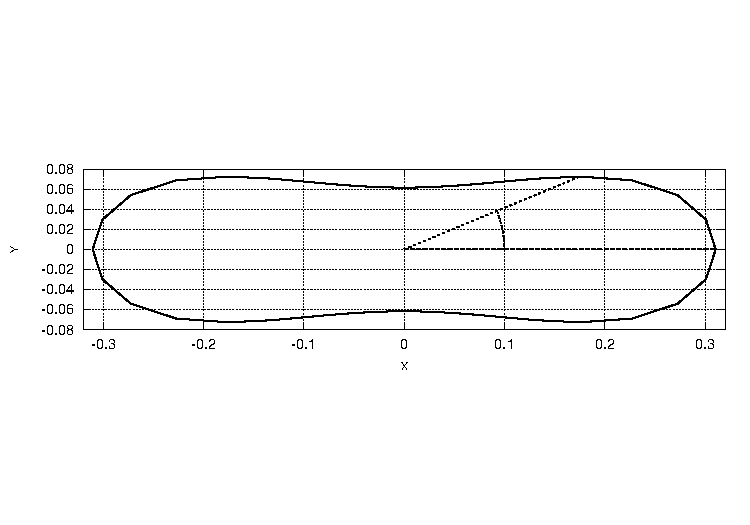
\includegraphics[width=\textwidth]{figures/orbit_theta_sup_1}
\caption{Hamiltonian orbit when $I>I_c$ and $K_{2I}<
K < K_s$}
\label{f:orbit_theta_sup_1}
\end{center}
\end{figure}

\begin{figure}
\begin{center}
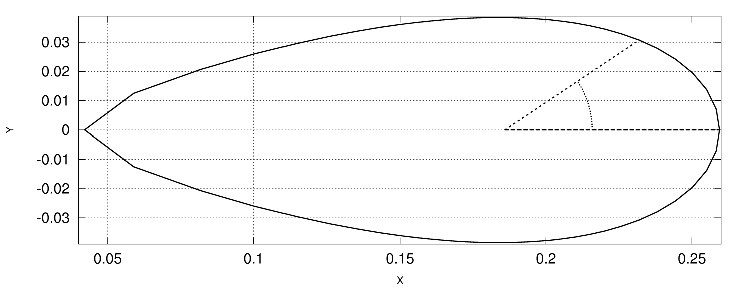
\includegraphics[width=\textwidth]{figures/orbit_theta_sup_2_cropped}
\caption{Hamiltonian orbit when $I>I_c$ and $K_s< K < K_e$}
\label{f:orbit_theta_sup_2}
\end{center}
\end{figure}

To apply~\eqref{e:polar integral}, $r(\theta)$ is calculated with a numerical root solver by transforming equation~\eqref{e:averaged K} to polar coordinates.

The procedure described above holds in the $K-I$ domain wherever the period is not infinite. The period is infinite along the edges $K_s$ and $\mathcal{K }_e$. Along the edge $K_s$ the diffusion coefficients have a finite value whereas the drift coefficients do not, but only the former need to be evaluated to impose the conservation of probability flux condition. Along the edge $\mathcal{K}_e$, the drift and diffusion coefficients are found by linearization about the coordinates of the elliptic fixed points. Sample representations of the drift and diffusion coefficients are shown in figure~\ref{f:drift diffusion figures}.

\begin{figure}
\begin{center}
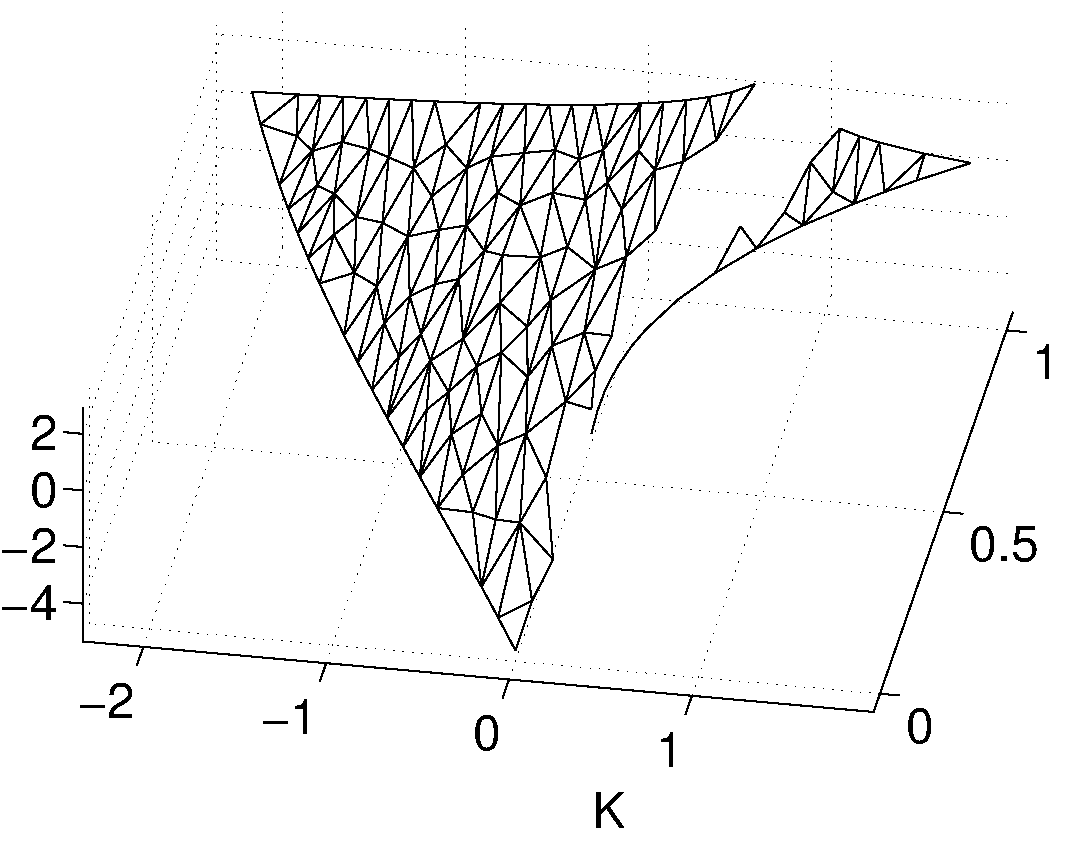
\includegraphics[width=\textwidth*7/16]{figures/b1_db4_mesh}
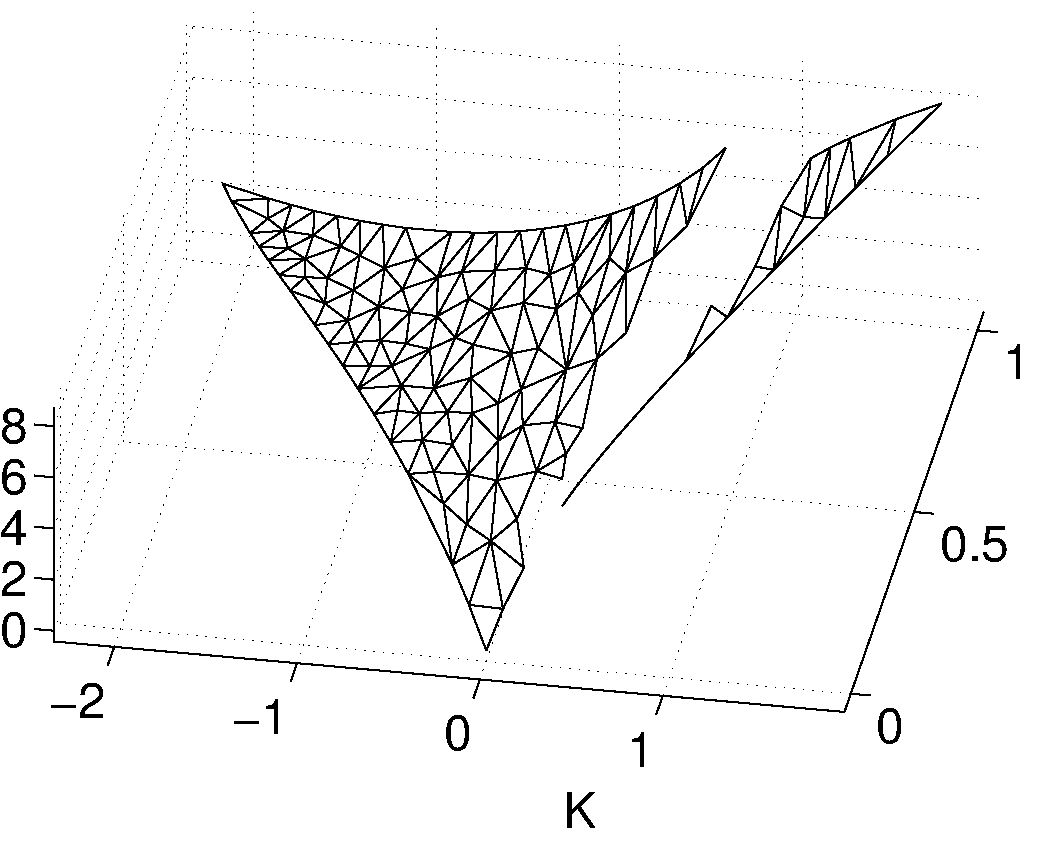
\includegraphics[width=\textwidth*7/16]{figures/a11_db4_mesh}
\caption{Drift $\mathring{\mathfrak b}_K$ (left) and diffusion $\mathring{\mathfrak a}_{\mathcal K \mathcal K}$ (right). Parameters are as follows: radius = 1, depth = 1, $\sigma_1 = -3$, $\sigma_2 = 0$, $\alpha_{1,2} = -0.25$, $\omega \mathcal{F}_c(\omega) = 25$}
\label{f:drift diffusion figures}
\end{center}
\end{figure}

\section{Conclusions}

In this chapter, it has been demonstrated that surface wave motion can be analyzed using stochastic averaging techniques. To achieve this a Hamiltonian model of surface wave motion was used to transform a set of governing partial differential equations into an infinite system of ordinary differential equations. Stochastic effects were then added to the model. Resonance was introduced and the geometry of the reduced graph of the stochastic process was established. Finally the averaged drift and diffusion coefficients were calculated throughout the domain. To do so, numerical algorithms were devised and special care was given to the boundaries of the reduced graph where singularities can manifest themselves.

With the drift and diffusion coefficients determined, a two-dimensional reduced Markov process has been characterized in the weak sense. In Chapter \ref{c:pdf}, our analysis continues. We will determine stationary probability density distributions associated with the generator of the surface waves problem.

% FIXME Freidlin's work suggests drift coefficient can be calculated along gluing edge

% FIXME Calculation at center edge _and_ I_c

% % Old Section
% To perform this quadrature, spatial averaging must be performed. First
% the orbits shown in Figures~\ref{f:X Y phase portrait I < I_c}
% and~\ref{f:X Y phase portrait} need to be computed with some
% accuracy. These orbits can be obtained in at least two ways. The first
% is to solve the equations for $\dot{X}_t$ and $\dot{Y}_t$
% (Equations~\eqref{e:Xdot} and~\eqref{e:Ydot}) as a set of ODEs,
% the second method is to calculate contour levels of the
% Hamiltonian. We do the latter using MATLAB's \emph{contourc}
% function. With this method, in order to maintain approximately the
% same accuracy throughout the domain $\mathfrak{G}$, it appears that
% the number of gridpoints on which $K$ is calculated and used
% as input to the function \emph{contourc} must be approximately the
% same for all orbits.
%
% \emph{Contourc} outputs a list of $X,Y$ coordinates at which
% $K$ has a specified value thus making it possible to
% calculate $\mathfrak{b}_i$ and $\mathfrak{a}_{jk}$.


\chapter{Autoparametric Oscillator}
\label{c:autoparametric}
\section{Introduction}
\label{S:introduction}
We investigate the random vibrations of a nonlinear stochastically-forced system of the form
\begin{equation}
\begin{aligned} 
\ddot q_1(t) + \zeta_1 \dot q_1(t) + f_1(q_1(t),q_2(t)) &= \xi (t)\\
\ddot q_2(t) + \zeta_2 \dot q_2(t) + f_2(q_1(t),q_2(t)) &= 0
\end{aligned}
\qquad t \ge 0
\label{E:2dof}
\end{equation}
where for each time $t > 0$, $(q_1(t), q_2(t))$ represents the generalized coordinates of the system, the constants $\zeta_1$ and $\zeta_2$ are damping coefficients, and $\xi$ is a stationary random process. While only the first mode $q_1$ is forced, the nonlinear coupling can transfer energy to the second mode $q_2$. Often, systems such as~\eqref{E:2dof} are known as \emph{autoparametric systems} (one may think of $q_1$ as a parameter in the dynamics of $q_2$). Our focus here is when the dynamics of $q_1$ and $q_2$ are that of coupled and damped oscillators, and we are then interested in questions of \emph{stability} of the stochastic system~\eqref{E:2dof}, and in particular we are interested in the transfer of energy from the forced mode to the unforced mode.

% Describe general form of autoparametric systems

Periodically excited autoparametric systems have been studied extensively; see for example \citet{sethna65:_vibrat_of_dynam_system_with_qudrat_nonlin, haxton72:_autop_vibrat_absor, nayfeh79:_nonlin_oscil, hatwal83:_forced_nonlin_oscil_of_autop_1, bajaj96:_amplit_modul_dynam} and \citet{tien94:_nonlin_dynam_of_shall_arch}. The most interesting situations occur when the natural frequencies of the excited mode and the unexcited mode are in 2:1 resonance. If the excitation is periodic and the energy of the forced oscillator is increased, it reaches a certain value of amplitude at which saturation takes place for the oscillator and the energy is transferred to the unforced second mode. This may be undesirable, because disturbances affecting one mode may cause unwanted instability in another mode. Our effort (which is not considered by any of the above works) is to study energy transfer in the presence of noisy input.

A natural question is whether such saturation and transfer of energy take place in the presence of stationary random excitations (as opposed to deterministic periodic excitations). Although various papers have dealt with some aspects of this question, non have given completely satisfactory answers. This is primarily due to the complex interactions between, noise, nonlinearities and resonances. Our approach is to study these interactions via a \emph{novel dimensional-reduction} approach. The analysis hinges upon some recent abstract theories of stochastic dimensional reduction. We then use this reduced model to calculate some essential design-related statistical measures of response and stability (e.g., mean exit times and stationary measures).

The important assumption in our analysis is that the dissipation and random perturbations be small. Of course this means that their effect will be visible only over a long time horizon. However, since the noise is small, the dynamics of the unperturbed system gives some structure to our analysis and organizing the effects of the random perturbation. In particular, the dynamics of the unperturbed system identify a reduced phase space (the orbit space) on which to carry out \emph{stochastic averaging}. While the classical theory of \emph{stochastic averaging} is a natural framework for such a program, the equations of interest contain \emph{resonance} and \emph{bifurcation}, which precludes a simple application of classical techniques. In particular, the resonance gives rise to an intermediate scale, and the bifurcations give rise to some non-standard singularities in the orbit space. Such an analysis allows us to carefully study the multivalent features of our system. See \citet{freidlin94:_random_pertur_of_hamil_system,freidlin98:_random_pertur_nonlin_oscil,namachchivaya01:_non_duffin_pol} and \citet{sowers02:_stoch_averag_with_flatt_hamil} for some related investigations.

\section{Physical Model}
\label{S:model}

The equations of motion~\eqref{E:2dof} considered can model the dynamics of a number of structural and mechanical systems, namely a randomly excited and initially deformed shallow arch, a suspended elastic cable driven by planar excitation, or a water vessel subject to longitudinal wave action. To keep things as simple as possible, we shall consider a very simple system, namely a type of \emph{autoparametric vibration absorber with randomly excited base} (see \citep{hatwal83:_forced_nonlin_oscil_of_autop_1}). Namely, we shall consider a mass attached by a spring to a pendulum, as illustrated in Figure~\ref{F:ap schematic}. For clarity, we use \emph{mass} to refer to the object at the free end of the spring, while the object at the end of the pendulum is referred to as the \emph{bob}. The quantity $\varphi$ is the angle of the pendulum (with respect to the vertical axis) and the quantity $y$ represents the height of the mass (relative to a rest position defined by the position of the pendulum). The mass is forced according to a stochastic signal $\Xi(t)$. The subscripts here refer to the fact that this is our original physical model. The equations for such a system can be written as
\begin{equation}
\label{e:absorber}
\begin{gathered}
(m_o + m_p) \ddot y + d_o \dot y + k y + m_p l (\ddot \varphi \sin \varphi + {\dot \varphi}^2 \cos \varphi) = \Xi\\
m_p l^2 \ddot \varphi + d_p \dot\varphi + m_p l (g + \ddot y) \sin \varphi = 0
\end{gathered}
\end{equation}
where $m_o$, $d_o$ and $k$ are the mass, damping and the spring constant of the spring-mass system and $m_p \,$, $d_p$ and $l$ are the mass, damping and the length of the pendulum.
\begin{figure}
\begin{center}
\includegraphics[width=\textwidth*7/8]{figures/schematic}
\caption{Schematic of the autoparametric system governed by equations~\eqref{e:absorber}. The letter ``o'' denotes the mass and ``p'' denotes the pendulum.}
\label{F:ap schematic}
\end{center}
\end{figure}
The kinetic and the potential energies of the conserved system are given by
\begin{gather*}
T \equiv \frac12 (m_o + m_p){\dot y}^2 + \frac12 m_p \, l^2 {\dot \varphi}^2 + m_p \, l \dot y \, \dot \varphi \sin \varphi\\
U \equiv m_p \, g l ( 1 -\cos \varphi) + \frac12 k y^2
\end{gather*}
It is clear that the nonlinearities in the equations of motion arise due to the gravitational restoring force and due to the dependence of kinetic energy on the angle $\varphi$ which leads to inertial coupling between the the two coordinates. It also turns out (we shall use this later) that in the absence of noise and damping, this system is Hamiltonian, so the dynamics of $y$ and $\varphi$ are governed by the geometry of this Hamiltonian.

In order to non dimensionalize the equations in system \eqref{e:absorber}, a change of variables is introduced:
\begin{align*}
t &= \tau/\omega_0, & y(t) &= l \hat \eta(\tau), & \varphi(t) &= \hat \theta(\tau), & \Xi(t) &= k l \hat \xi(\tau).
\end{align*}
$\omega_o$ is defined by
\[
\omega_o^2 = \frac{k}{m_o + m_p}
\]
Then
\begin{align*}
\frac{dy(t)}{dt} &= l \frac{d \hat \eta(\tau)}{d \tau} \frac{d \tau}{d t}\\
&= l \omega_o \frac{d \hat \eta(\tau)}{d \tau}
\end{align*}
\[
\frac{d^2y(t)}{dt^2} = l \omega_o^2 \frac{d^2 \hat \eta(\tau)}{d \tau^2}
\]
\[
\frac{d \varphi(t)}{dt} = \omega_o \frac{d \hat \theta(\tau)}{d \tau}
\]
\[
\frac{d^2 \varphi(t)}{dt^2} = \omega_o^2 \frac{d^2 \hat \theta(\tau)}{d \tau^2}
\]
Substituting into the equation for $y$ in \eqref{e:absorber} gives
\[
\ddot{\hat \eta} + \frac{d_o}{\sqrt{k}\sqrt{m_o + m_p}} \dot{\hat \eta} + \hat \eta + \frac{m_p}{m_o + m_p} (\ddot{\hat \theta} \sin \hat \theta + {\dot{\hat \theta}}^2 \cos \hat \theta) = \hat \xi
\]
Two dimensionless quantities follow naturally:
\begin{align*}
\hat \zeta_o &= \frac{d_o}{2 \sqrt{k} \sqrt{m_o + m_p}} & R &= \frac{m_p}{m_o + m_p}
\end{align*}
The equation for $\ddot{\hat \eta}$ becomes
\[
\ddot{\hat \eta} + 2 \hat \zeta_o \dot{\hat \eta} + \hat \eta + R(\ddot{\hat \theta} \sin \hat \theta + {\dot{\hat \theta}}^2 \cos \hat \theta) = \hat \xi
\]
The equation for $\varphi$ when non dimensionalized becomes
\[
m_p l^2 \omega_o^2 \ddot{\hat \theta} + d_p \omega_o \dot{\hat \theta} + m_p l^2 \omega_0^2 (\frac{g}{l \omega_o^2} + \ddot{\hat \eta}) \sin \hat \theta = 0.
\]
Substituting for $\omega_o$, $\omega^2 = g/l$ and $q = \omega/\omega_o$ gives
\[
R \ddot{\hat \theta} + \frac{d_p}{l^2 \sqrt{k} \sqrt{m_o + m_p}} \dot{\hat \theta} + R (q^2 + \ddot{\hat \eta}) \sin \hat \theta = 0
\]
Introducing a third nondimensional quantity:
\[
\hat \zeta_p = \frac{d_p \sqrt{m_o + m_p}}{2 l^2 m_p \sqrt{k}} = \frac{d_p}{2 l^2 m_p \omega_o},
\]
the equation for $\hat \theta$ becomes
\[
R \ddot{\hat \theta} + 2 R \hat \zeta_p \dot{\hat \theta} + R (q^2 + \ddot{\hat \eta}) \sin \hat \theta = 0
\]
The corresponding Lagrangian for the autonomous and non-dissipative system is
\begin{equation}
\label{E:lagrangian}
L = \frac12 {\dot{\hat\eta}}^2 + \frac12 R {\dot{\hat\theta}}^2 + R {\dot{\hat\eta}}\,{\dot{\hat\theta}}\,\sin \hat{\theta} - \frac12 {\hat \eta}^2 - R q^2 \left(1 - \cos \hat{\theta} \right)
\end{equation}
Making use of the velocities in terms of the generalized momentum, we
have
\begin{equation}
\label{E:velocity}
\dot {\hat \eta} = \frac {p_1 - p_2\,\sin \hat{\theta} }{1-R \sin^2 \hat{\theta} },\quad \dot {\hat \theta} = \frac {p_2- R \, p_1\,\sin \hat{\theta} }{R\left(1- R \sin^2 \hat{\theta} \right)}
\end{equation}
and from Legendre transformation we obtain the Hamiltonian as
\[
H = \frac12 \frac{{p_1}^2}{1 - R \sin^2 \hat{\theta}} - \frac{p_1 p_2 \sin \hat{\theta}}{1- R \sin^2\hat{\theta}} + \frac12 \frac{{p_2}^2}{R (1 - R \sin^2\hat{\theta})} + \frac12 \hat{\eta}^2 + R q^2 (1 - \cos\hat{\theta}).
\]
When $\hat\xi$ is periodic, the motion of the mass causes variations in the absorber spring stiffness, and in turn, the absorber acts (in a nonlinear fashion) back on the main mass. With appropriate choice of tuning parameters, the effect of the mass can be completely absorbed. For periodically excited autoparametric systems, the most interesting situations occurs when the natural frequencies of the mass and the pendulum are in $2:1$ internal resonance; i.e., when $q = 1/2$. In resonance, the pendulum is primarily excited by energy coming from the mass. When the external energy put into the mass is small enough, its effect on the pendulum is small compared to the stability of the hanging pendulum. As the external energy increases, a saturation takes place at a certain threshold, above which the pendulum noticeably moves; see \citep{nayfeh79:_nonlin_oscil}. In some mechanical absorbers, this transfer of energy is useful. In other systems, it may not, since a disturbance affecting one mode may cause unwanted dynamics in other modes (for example, longitudinal wave action could lead to capsizing of a ship). Since such disturbances often contain an essential \emph{random} component (think of water waves in the ocean), it is essential to complement the above investigations of the effect of periodic excitations by corresponding investigations of the effect of random excitations.

Our interest here is a refined stability analysis near the fixed point $(\hat\eta,\hat\theta)\equiv 0$ of the unperturbed system. In particular, we are interested in the effect of small random perturbations, so we will let $\hat\xi$ be of the form $\hat\xi = \epsilon^2 \nu \xi$, where $\xi$ is a noise process of ``unit'' variance and $\nu$ is some empirical parameter. Our dynamics are most interesting when they are not overdamped, so let $\hat\zeta_o$ and $\hat\zeta_p$ be of the form $\hat\zeta_o = \epsilon^2 \zeta_o$ and $\zeta_p = \epsilon^2 \zeta_p$, where $\zeta_o$ and $\zeta_p$ are some positive constants (this corresponds to letting $d_o$ and $d_p$ be of size $\epsilon$). Guided by the corresponding analysis for periodic forcing, we are interested in the behavior when $q^2$ is very close to $q^2_o\equiv 1/4$. Let's replace $q$ by $q_o + \epsilon^2 \mu$, where $\mu$ is an unfolding parameter. Since we are interested in $\hat\eta$ and $\hat\theta$ near the fixed point $0$, we should look at these quantities on a finer resolution. Namely, let $\eta$ and $\theta$ be defined by
\[
\hat\eta(t) = \epsilon \eta(t) \qquad \hat\theta(t) = \epsilon \theta(t)
\]
Then the dynamics of our system are
\begin{equation}
\begin{aligned} 
\ddot \eta + 2 \epsilon^2 \zeta_o \dot \eta + \eta + R (\ddot\theta \sin(\epsilon\theta) + \epsilon \dot\theta^2 \cos (\epsilon\theta) ) &= \epsilon\nu\xi\\
\ddot \theta + 2 \epsilon^2 \zeta_p \dot \theta + \left( \left(q_o + \epsilon^2 \mu\right)^2 \frac{\sin (\epsilon \theta)}{\epsilon} + \ddot \eta \sin (\epsilon\theta) \right) &= 0.
\end{aligned}
\label{E:dynamics}
\end{equation}

The salient feature of this system is that the dominant deterministic component of the dynamics gives us a place to start to search for structure in the light of randomness. Once we understand this structure, we can then investigate how various system parameters (i.e., the damping coefficients, $R$, $\nu$ and $\mu$) affect various important engineering quantities -- exit times from stable regions, invariant measures, etc.

\section{Single Mode Solutions}
\label{S:single}

To clarify some general qualitative effects of noise, let's consider a simple stability analysis using some spectral methods and the first-order linearization. Assume that initially the pendulum hangs vertically, at rest. Then $\theta$ will be identically zero -- ``locked-mass'' dynamics. The mass on the spring can move only in the vertical direction and is excited by $\nu \xi$. We get the equation
\[
\ddot \eta + 2 \epsilon^2 \zeta_o \dot \eta + \eta = \epsilon \nu \xi.
\]
If $\xi$ is white noise we can solve for $\eta$ explicitly. Its power spectral density is
\[
S_\eta(\omega)=\frac{\epsilon^2\nu^2 S_0}{(1-\omega^2)^2+4\epsilon^4\zeta_o^2 \omega^2}
\]
where $S_0$ is the power spectral density of $\xi$. The peak intensity and the carrying frequency of $\eta$ are determined by the filter parameter $\zeta_o$.

The stability of the locked mass steady-state oscillation is now obtained by using the first-order approximation of sine and cosine in the dynamics for $\theta$. We get
\[
\ddot \theta + 2 \epsilon^2 \zeta_p \dot \theta + ( (q_0+\epsilon^2\mu)^2 + \epsilon \ddot \eta ) \theta =0
\]
and the power spectral density of $\ddot\eta$ is given by
\[
S_{\ddot \eta} (\omega) = \frac {\omega^4 \epsilon^2 \nu^2 S_0}{(1 - \omega^2)^2 + 4 \epsilon^4 \zeta_o^2 \omega^2}
\]
The maximal Lyapunov exponent can now be easily calculated and the stability boundary can be obtained in terms of excitation intensity $\nu$ and the dissipation coefficients $\zeta_p$. An explicit expression for the maximal Lyapunov exponents of the single mode solution is given
in \citet{arnold86:_asymp_analy_lyapun_expon} and \citet{namachchivaya87:_stoch_pertur_hopf_bifur}; expanding it in $\epsilon$, we have
\[
\lambda_1 \approx \epsilon^2 \left( - \zeta_p + \frac{1}{8 \, q_o^2} S_{\ddot \eta}(2 \,(q_o+\epsilon^2\mu))\right)
\]
Using the trace formula, the second Lyapunov exponent can be obtained as
\[
\lambda_2 = \epsilon^2 \left( - \zeta_p - \frac{1}{8 \, q_o^2} S_{\ddot \eta}(2 \,(q_o+\epsilon^2\mu)) \right).
\]
The noise has no effect on the other two exponents; i.e., $\lambda_3=\lambda_{4}= - \zeta_o$.

At exact one-to-two resonance, i.e., $\mu=0$, the maximal Lyapunov exponent reduces to
\begin{equation}
\lambda_1 = \epsilon^2 \left( - \zeta_p + \frac{{\nu}^2 \, S_0}{8 \, \zeta_o^2} \right)
\end{equation}
It is clear, that when the noise intensity $\nu^2$ is small (remember that we have normalized so that $\xi$ has unit intensity), the size of the oscillations of $\eta$ is similarly small. Since the point $\theta\equiv 0$ is a stable point for the hanging pendulum, the pendulum undergoes small random motion near $\theta\equiv 0$, and all four Lyapunov exponents are negative. However, as we further increase the noise intensity, the top exponent becomes positive when $\nu^2 S_0 = 8 \zeta_o^2 \zeta_p$. The system then becomes unstable, and a host of questions arise.
\begin{itemize}
\item Do both the mass spring oscillator and the pendulum undergo random vibrations when the top exponent becomes positive~(i.e., ${\nu}^2 \, S_{0} > 8\,\zeta_o^2\,\zeta_p$), i.e., does a new coupled-mode ``stationary solution'' or ``stationary density function'' appear?
\item Does the positive exponent lead to a transfer of energy from the mass to the vertically hanging pendulum, i.e., is the energy transferred only after the mean square amplitude of the motion of the mass reaches a certain critical size?
\end{itemize}

\section{Coupled Mode Problem}
\label{S:statement}

The deficit of the above analysis is that it relied upon simplifying linearizations. The true dynamics of $y$ and $\theta$ are of course globally governed by nonlinear effects. It is to an analysis of these nonlinear effects that we commend ourselves in this paper. Namely, in order to maintain the nonlinear nature of the dynamics of $y$ and $\theta$, we will keep all terms which are of order $\epsilon^2$ and larger.

Before writing out the exact equations, let's invoke some of the formalism of mechanics. We can rewrite~\eqref{E:dynamics} in terms of the generalized coordinates ($\eta, \theta$) and conjugate momenta ($p_1, p_2$) are expressed as
\[
\begin{aligned}
\dot \eta &= \frac{p_1 - p_2\sin (\epsilon \theta)}{1-R\sin^2(\epsilon \theta)}\\
\dot \theta &= \frac{p_2 - Rp_1\sin (\epsilon \theta)}{R(1-R\sin^2(\epsilon \theta))} \\
\dot p_1 &= -\eta - 2 \epsilon^2 \zeta_o\left(\frac{p_1 - p_2\sin (\epsilon \theta)}{1-R\sin^2(\epsilon \theta)}\right) + \epsilon \nu \xi\\
\dot p_2 &= R\epsilon \left(\frac{p_1 - p_2\sin (\epsilon \theta)}{1-R\sin^2(\epsilon \theta)}\right)\left(\frac{p_2 - Rp_1\sin (\epsilon \theta)}{R(1-R\sin^2(\epsilon \theta))}\right)\cos(\epsilon \theta) \\
&\qquad - R (q_0 + \epsilon^2 \mu)^2\frac{\sin (\epsilon \theta)}{\epsilon} - 2 \epsilon^2 R \zeta_p \left(\frac{p_2 - Rp_1\sin (\epsilon \theta)}{R(1-R\sin^2(\epsilon \theta))}\right)
\end{aligned}
\]
Expanding the sines and cosines and keeping terms up to order $\epsilon^2$, we get the system
\begin{gather*}
\dot \eta = p_1 - \epsilon p_2 \theta + \epsilon^2 R p_1 \theta^2\\
\dot \theta = \frac{p_2}{R} - \epsilon p_1 \theta + \epsilon^2 p_2 \theta^2\\
\dot p_1 = -\eta - 2 \epsilon^2 \zeta_o p_1 + \epsilon \nu \xi\\
\dot p_2 = -R q_0^2 \theta + \epsilon p_1 p_2 + \epsilon^2 \left\{\frac{1}{6} R q_0^2 \theta^3 - 2 R q_0 \mu \theta - R p_1^2 \theta - p_2^2 \theta - 2 \zeta_p p_2\right\}
\end{gather*}
and the Hamiltonian is
\begin{multline*}
\label{e:hamiltonian}
H = \frac{p_1^2}{2} + \frac{p_2^2}{2R^2} + \frac{\eta^2}{2} + \frac{Rq_0^2\theta^2}{2} - \epsilon p_1 p_2 \theta\\ + \epsilon^2\left\{\frac{p_2^2 \theta^2}{2} + \frac{R p_1^2\theta^2}{2} - \frac{R q_0^2 \theta^4}{24} + R q_0 \mu \theta^2 \right\}
\end{multline*}
The dominant dynamics of $\eta$ and $\theta$ are
\[
\ddot \eta + \eta = 0 \qquad \text{and}\qquad \ddot \theta + q_0^2 \theta = 0
\]
We apply the following time dependent symplectic transformation:
\begin{gather*}
\eta = x_1 \cos t + x_3 \sin t\\
p_1 = -x_1 \sin t + x_3 \cos t \\
\theta = [x_2 \cos (q t) + x_4 \sin (q t)]/\sqrt{R q}\\
p_2 = \sqrt{R q}\, [-x_2 \sin (q t) + x_4 \cos (q t)]
\end{gather*}
The conjugate pairs are $(x_1,x_3)$ and $(x_2,x_4)$. Then $\boldsymbol x = (x_1,x_2,x_3,x_4)$ satisfies the random evolution equation
\begin{equation}
\dot{\bm x}^\epsilon_t = \epsilon \bm b^1(\bm x^\epsilon_t,t) + \epsilon^2 \bm b^2(\bm x^\epsilon_t,t:\zeta,\mu) + \epsilon \bm \sigma(\bm x^\epsilon_t, t: \nu) \xi(t)
\label{E:standard1}
\end{equation}
where $b^1$ contains spatially quadratic nonlinearities (which come from a cubic Hamiltonian) and $b^2$ contains spatially cubic nonlinearities (arising from a quartic Hamiltonian), and terms arising from dissipation and detuning. The explicit form of the quadratic and cubic nonlinear terms are given in Appendix~\ref{A:autoparam nonlin vec fields}. The stochastic forcing terms are defined by
\[
\bm \sigma(x,t:\nu) = \{-\nu \sin t, 0, \nu \cos t, 0\}
\]

It is important to realize that there are three scales in~\eqref{E:standard1}. The periodicity of the coefficients appears on time intervals of order $1/\epsilon$. The terms containing $b^2$ and $\sigma$ cause fluctuations of order $\epsilon$ and $\sqrt{\epsilon}$. The effect of the $b^1$ term is to cause fluctuations of order 1. Our interest here is when the periodic fluctuations of the coefficients in a sense cancel out the fluctuations due to $b^1$, leaving us with fluctuations of order $\epsilon$.

\subsection{Conserved Quantities}
\label{S:averagedequations}

From the explicit formulas for $b^1$ in Appendix~\ref{A:autoparam nonlin vec fields} (where $q=1/2$), we see that for $x = (x_1,x_2,x_3,x_4) \in \Real^4$,
\[
(\Tave b^1)(x) =
\begin{pmatrix}
-\frac12 x_2x_4 \\
\frac12 (x_1 x_4 - x_2 x_3)\\
\frac14 (x_2^2-x_4^2)\\
\frac12 (x_1 x_2 + x_3 x_4)
\end{pmatrix}
\]
The Hamiltonian associated with these dynamics is
\begin{equation}
\label{E:Hamiltonian}
K(\boldsymbol x) = \frac14 x_1(x_4^2 - x_2^2) - \frac12 x_2 x_3 x_4
\end{equation}
The Hamiltonian system
\begin{equation}
\label{E:flow}
\dot{z} = \bar{\nabla} K(z)
\end{equation}
has a second integral which is in involution with the Hamiltonian \eqref{E:Hamiltonian} (two integrals of motion are in involution if their Poisson bracket vanishes identically). Thus, the unperturbed four-dimensional Hamiltonian has \emph{two first integrals in involution}, namely, the Hamiltonian itself \eqref{E:Hamiltonian} and a second invariant or constant of motion (momentum variable)
\begin{equation}
\label{E:momentum}
I(x)=(x_1^2+x_3^2)+\frac12\,(x_2^2+x_4^2).
\end{equation}
The invariant $I$ is functionally independent of $K$, exists globally and is single valued. 

\subsection{Structure of the Unperturbed Systems}
\label{S:Unperturbed}

Our main analytical tool is a certain method of \emph{dimensional reduction} of nonlinear systems with symmetries and small noise. As the noise becomes asymptotically small, one can exploit symmetries and a separation of scales to use well-known methods (viz. stochastic averaging) to find an appropriate lower-dimensional description of the system.

Consider the following symplectic transformation
\begin{align*}
x_1 &= \sqrt{2 J}\sin(\phi + 2 \psi) & x_3 &= \sqrt{2 J} \cos(\phi + 2 \psi)\\
x_2 &= \sqrt {2 (I - 2 J)}\sin \psi & x_4 &= \sqrt{2(I - 2J)} \cos \psi
\end{align*}
The conjugate pairs are $(\phi,J)$ and $(\psi,I)$. This transformation yields a new set of equations which can easily be integrated
\begin{equation}
\label{E:vector-trans}
\begin{aligned}
\dot \phi_t &= \frac{\sqrt{2J_t}}{4J_t} (I_t - 6 J_t) \sin \phi_t & \dot J_t &= \frac{\sqrt{2 J_t}}{2} (2 J_t - I_t) \cos \phi_t\\
\dot \psi_t &= \frac{\sqrt{2 J_t}}{2} \sin(\phi_t) & \dot I_t &= 0
\end{aligned}
\end{equation}
The Hamiltonian corresponding to the equations above is
\[
K = \frac{\sqrt{2 J}}{2} (I-2 J)\sin \phi
\]
If $\psi_t$ is a solution, then $\pi + \psi_t$ is also a solution. Further, it is clear from~\eqref{E:vector-trans} that at exact resonance, during the undamped motion, the energy in the system continues to be exchanged between the two modes of oscillation provided the initial conditions are not on the circle $J = I/2$. However, the dynamics on that plane ($x_2=x_4=0$) in the original coordinates, which corresponds to the circle $J=I/2$, is given by
\[
\dot \phi_t = - \sqrt{I_0} \sin \phi_t, \quad \dot \psi_t =
\frac{\sqrt{I_0}}{2} \sin \phi_t,
\qquad I=I_0, \quad J= \frac{I_0}{2}
\]
Hence, the plane~($x_2=x_4=0$) is invariant and for initial conditions on the the circle $J=I/2$~(heteroclinic orbit), the energy exchange is not periodic.

To make the calculations even simpler, we consider the symplectic transformation
\begin{equation}
\label{E:combin_transf}
\begin{aligned}
x_1 &= u_1 \cos(2 \psi) + u_2 \sin(2 \psi), & x_3 &= -u_1 \sin(2 \psi) + u_2 \cos(2 \psi)\\
x_2 &= \sqrt {2 (I-u_1^2-u_2^2)} \sin \psi, & x_4 &= \sqrt {2 (I - u_1^2 - u_2^2)} \cos \psi.
\end{aligned}
\end{equation}
The conjugate pairs are $(u_1,u_2)$ and $(\psi,I)$. This transformation yields
\begin{align}
\label{E:vector-int}
\dot u_{1t} &= - {u_1}_t {u_2}_t , & \dot u_{2t} &= \frac12 (3 {u_1}_t^2 + {u_2}_t^2 -I_t), & \dot \psi_t &= \frac12\,{u_1}_t, \quad \dot I_t = 0
\end{align}
and the corresponding Hamiltonian is
\begin{equation}
K = \frac12 u_1 \left(I - (u_1^2 +u_2^2)\right)
\label{E:AvgH}
\end{equation}
System~\eqref{E:vector-int} has four fixed points. They are
\begin{align*}
(u_1, u_2) &= (0, \pm \sqrt{I}) & (u_1, u_2) &= (\pm \frac{\sqrt{3 I}}{3}, 0)
\end{align*}
\begin{figure}
\begin{center}
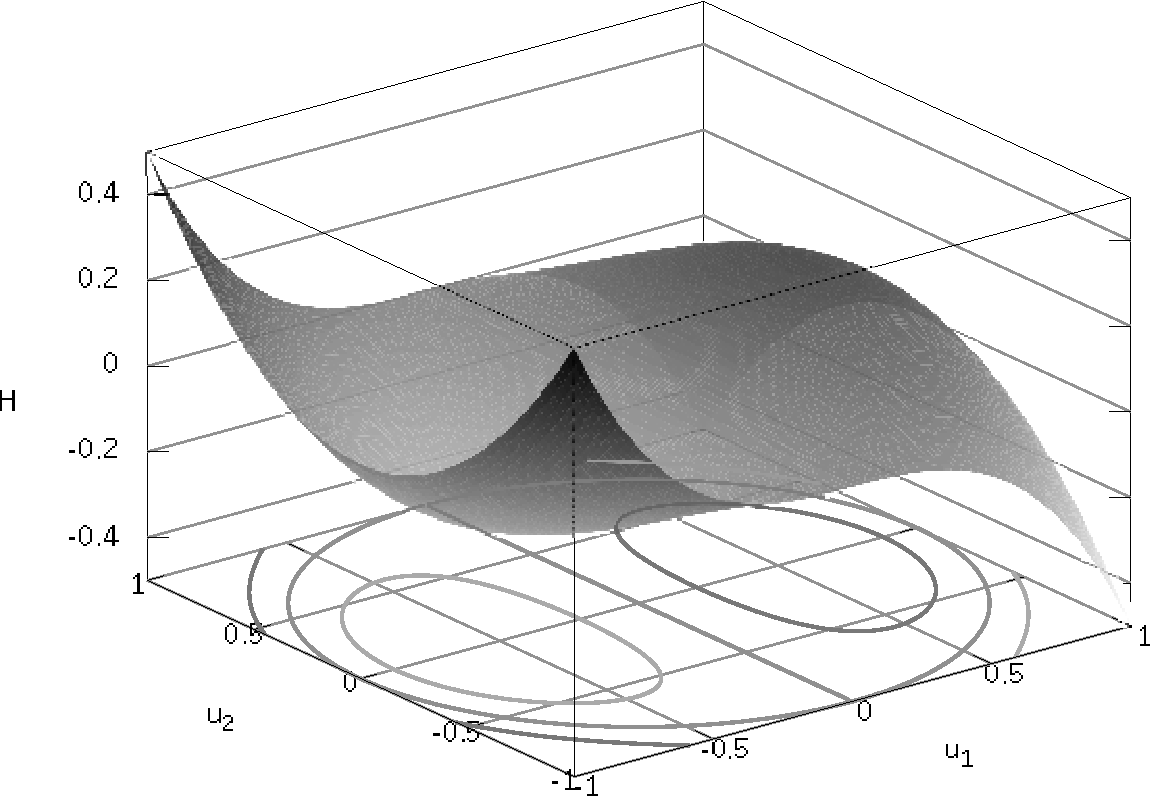
\includegraphics[width=\textwidth]{figures/h_surf}
\caption{Surface and contour plots of the averaged Hamiltonian in $u_1,u_2$ coordinates, as given in~\eqref{E:AvgH}. $I = 1$.}
\label{f:autoparam Hamiltonian}
\end{center}
% FIXME Surface should be restricted to $u_1^2 + u_2^2 \le 2 I$
\end{figure}

% FIXME The transformation below is not canonical and the variables z haven't been introduced
% Combining the transformations~\eqref{E:vector-trans}
% and~\eqref{E:sym-trans3} yields
% \begin{align} 
%  z_1 &= u_1 \cos \Theta + u_2 \sin \Theta &
%  z_2 &= \sqrt{2(I - u_1^2 - u_2^2)} \sin (\Theta/2)\notag\\
%  z_3 &= - u_1 \sin \Theta + u_2 \cos \Theta &
%  z_4 &= \sqrt{2(I - u_1^2 - u_2^2)} \cos (\Theta/2)
% \label{E:combin_transf}
% \end{align}
% where $\Theta= t + 2 \psi$ and ~\eqref{E:combin_transf} can be used to
% interpret the results of the averaged equations in terms of the
% original equations.

As $I$ varies, the system described by \eqref{E:vector-int} can display bifurcations. At exact resonance, by using the action-angle coordinates, we express the non-dissipative deterministic flow as
\begin{equation}
\label{E:hamilflow}
\begin{aligned}
\dot z_t^I(u) &= \bar{\nabla} K(z_t^I(u), I), \quad z_0^I(u)=u =(u_1,u_2)\\
\psi &= \int_{0}^{t} {D_{I} K(z_t^I(u), I) \ ds} + \psi_{0} \\ K
&= \text{constant} \in \Real, \quad I = \text{constant} \in \Real^+
\end{aligned}
\end{equation}
The dynamics in the $u$-space are completely integrable and represent a one parameter family of an one degree of freedom Hamiltonian system. The fixed points and the corresponding energy levels for the unperturbed system are given by
\begin{equation}
\begin{aligned}
A^\pm: (\bar u_1^{0}, \bar u_2^\pm) &= (0, \pm \sqrt{I}), \quad K_{A^\pm} = 0 \\
B^\pm: (\bar u_1^\pm, \bar u_2^{0}) & = (\pm \sqrt{\frac{I}{3}},0),  K_{B^\pm} = \pm\frac{I}{3}\sqrt{\frac{I}{3}}
\end{aligned}
\label{E:fixed-points}
\end{equation}
provided $ I \ge 0 $. The eigenvalues are given by $\pm \sqrt{\bar u_2^2-3 \bar u_1^2 }$. For $I > 0$, $A^\pm$ represent saddle points while $B^\pm$ represent center fixed points and at $I = 0$ all four fixed points coalesce at the origin and both the eigenvalues are zero. It follows from transformations~\eqref{E:combin_transf} that $0 \le u_1^2+u_2^2 \le I$. Hence, the domain of interest is restricted to the area within and including the heteroclinic orbits; the periodic orbits encircling the two elliptic fixed points and the heteroclinic orbits.

Note that at the origin, the reduced domain has a cusp since
\begin{align*}
K &= \frac{I}{3}\sqrt{\frac{I}{3}} & \text{and}&&\eval{\frac{dK}{dI}}_{I=0} &= 0.
\end{align*}

\section{Time-Averaging}
\label{S:T-Average}

We have pointed out that that there are three time-scales involved in our averaging problems. According to the theory presented in Section \ref{s:stochatic averaging theory}, the first step is to average the periodic fluctuations of the coefficients and obtain $\Tave$-averaged quantities as the precursors to the stochastically averaged drift and diffusion coefficients. Somewhat laborious calculations yield
\begin{equation}
\begin{aligned}
m_1(x) &\equiv \left(\Tave \left(F_1^2 + \mathfrak{f}_1 + \mathfrak{g}_1\right)\right)(x)\\
&=-\frac{1}{32R}\left( \left(x_4^2-x_2^2 \right)x_3+2 x_2x_4x_1\right)\left(6R\left( x_1^2+x_3^2 \right)-x_2^2-x_4^2\right) \\
&\quad -(\zeta_o+2\,\zeta_p) K +\frac12\mu x_3(x_2^2-x_4^2) - \mu x_1x_2x_4\\
m_2(x)&\equiv\left(\Tave \left(F_2^2 + \mathfrak{f}_2 + \mathfrak{g}_2\right)\right)(x)\\
&= 2 \sigma^2S_{\xi\xi}(1) -2\zeta_o(x_1^2+x_3^2) - \zeta_p(x_2^2 + x_4^2)
\end{aligned}
\label{E:drift1}
\end{equation}
\begin{equation}
\begin{aligned}
a_{11}(x) &\equiv \left(\Tave \left(\sigma\sigma^T\right)_{11}\right)(x)\\
&= \frac{1}{32}\sigma^2S_{\xi\xi}(1)\left(x_2^2 + x_4^2\right)^2\\
a_{12}(x) &\equiv \left(\Tave \left(\sigma\sigma^T\right)_{12}\right)(x)\\
&= \sigma^2S_{\xi\xi}(1) K\\
a_{22}(x) &\equiv \left(\Tave \left(\sigma\sigma^T\right)_{22}\right)(x)\\
&= 2\sigma^2S_{\xi\xi}(1)\left(x_1^2+x_3^2\right)
\end{aligned}
\label{E:diffusion1}
\end{equation}
The symplectic transformation of \eqref{E:combin_transf} provides a convenient geometric structure of the unperturbed integrable Hamiltonian problem. In $(u,K,I)$ coordinates, the drift \eqref{E:drift1} and diffusion \eqref{E:diffusion1} coefficients are
\begin{equation}
\begin{aligned}
m_1(u,y) &= -(\zeta_o + 2\zeta_p) K\\
&\quad + \frac{1}{8 R} \left(u_1^2+u_2^2-I \right) u_2 \left(u_1^2+u_2^2-I + 3 R \left( u_1^2+u_2^2 + \frac{8 \mu}{3} \right) \right) \\
&= -(\zeta_o + 2\zeta_p) K - \frac14 \left(8\mu + 3I\right) K \frac{u_2}{u_1} + \frac12\left(3 + \frac{1}{R}\right)K^2 \frac{u_2}{u_1^2}\\
m_2(u,y) &= 2[\sigma^2 S_{\xi\xi}(1) - \zeta_o I + 2 (\zeta_o - \zeta_p) K/u_1]
\end{aligned}
\label{E:drift2}
\end{equation}
\begin{equation}
\begin{aligned}
a_{11}(u,y) &=\frac{1}{8} \sigma^2 S_{\xi\xi}(1) \left(u_1^2 + u_2^2 - I \right)^2\\
&= \frac12 \sigma^2 S_{\xi\xi}(1) K^2 \frac{1}{u_1^2}\\
a_{12}(u,y) &= \sigma^2 S_{\xi\xi}(1) K\\
a_{22}(u,y) &= 2 \sigma^2S_{\xi\xi}(1) (u_1^2 + u_2^2)\\
&= 2 \sigma^2 S_{\xi\xi}(1) (I - 2 K/u_1).
\end{aligned}
\label{E:diffusion2}
\end{equation}
Since, there are certain advantages in the use of one form of $m_{i}(u,y)$ and $a_{ij}(u,y)$ over the other, we shall make use of either one of the forms in evaluating the diffusion coefficients.

To obtain a limiting generator for the martingale problem, we need an averaging operator where the averaging is done with respect to the invariant measure concentrated on the closed trajectories.

In the deterministic context Neistadt's condition ~\citep{neistadt75:_passag_throug_reson_in_two_frequen_probl, neistadt75:_averag_in_multi_frequen_system,lochak88:_multip_averag_for_class_system} ensures the existence of an average transverse force that drives the trajectories away from the resonance zones. For the stochastic case, it was shown~\citet{ramakrishnan00:_near_reson_motion_of_random} that even for the case when Neistadt's condition does not hold, passage of trajectories through resonance without getting captured can be ensured if appropriate conditions on the noise are satisfied.

Using \eqref{E:drift2} in the $\Aave$-averaging operator yields on each leaf $\Gamma_i$, for $y=(K,I) \in \Gamma_i$,
\begin{gather}
\begin{split}
\mathfrak b_1^i &= \frac{1}{\period_i(y)}\int_{0}^{\period_i(y)} m_1(u(t),y) dt\\
&= -(\zeta_o+2\zeta_p) K -\frac14 (8\mu + 3I) K \frac{1}{\period_i} \int_0^{\period_i} \frac{u_2(t)}{u_1(t)} dt\\
&\quad + \frac12 \Bigl(3 + \frac{1}{R} \Bigr) K^2
\frac{1}{\period_i} \int_{0}^{\period_i}
\frac{u_2(t)}{{u_1(t)}^2} dt\\
&= -(\zeta_o + 2\zeta_p) K
\end{split}
\label{E:drift h}\\
\begin{split}
\mathfrak b_2^i & = \frac{1}{\period_i(y)}\int_{0}^{\period_i(y)} m_2(u(t),y) dt\\
& = 2 [\sigma^2 S_{\xi\xi}(1) - \zeta_o I] + 4(\zeta_o-\zeta_p) K
\frac{1}{\period_i}\int_{0}^{\period_i}\frac{dt}{u_1(t)}\\
& = 2 [\sigma^2 S_{\xi\xi}(1) - \zeta_o I] + 4(\zeta_o-\zeta_p) K \frac{\INT_{i}^1}{\period_i}
\end{split}
\end{gather}
\begin{gather}
\begin{split}
\Aa_{11}^i & = \frac{1}{\period_i(y)}\int_{0}^{\period_i(y)} a_{11}(u(t),y) dt\\
&= \frac12 \sigma^2 S_{\xi\xi}(1) K^2 \frac{1}{\period_i}\int_0^{\period_i}
\frac{1}{{u_1(t)}^2}dt\\
&=\frac12\,{\sigma}^2S_{\xi\xi}(1){K}^2\,\frac{\INT_{i}^2}{\period_i}
\end{split}\\
\begin{split}
\Aa_{12}^{i} &= \frac{1}{\period_i(y)}\int_{0}^{\period_i(y)} a_{12}(u(t),y)dt\\
&= \sigma^2 S_{\xi\xi}(1) K
\label{E:diffusion hi}
\end{split}
\\
\begin{split}
\Aa_{22}^i &= \frac{1}{\period_i(y)} \int_0^{\period_i(y)} a_{22}(u(t),y)dt\\
&= 2 \sigma^2 S_{\xi\xi}(1) \left(I - \frac{2 K}{\period_i} \int_0^{\period_i} \frac{1}{u_1(t)}dt \right)\\
&= 2 \sigma^2 S_{\xi\xi}(1) (I - 2 K \frac{\INT_i^1}{\period_i})
\end{split}
\end{gather}
We want to put these $\gen_i$'s together to get a Markov process on $\Graph$ with generator $\gen^\dagger_\Graph$ with domain $\mathscr{D}^\dagger_\Graph$, where $\Graph$ has a shape of an \emph{arrowhead}. For notational convenience, we also define $f_i \equiv f\big|_{\mathfrak{I}_i}$ for all $1\le i\le 2$. From the results of \citet{freidlin98:_random_pertur_nonlin_oscil}, and \citet{sowers03:_stoch_averag_near_homoc_orbit}, it is clear the gluing conditions, which we need to specify at the interior edges, solely depend on the diffusion coefficients $\Aa_{jk}^{i}$. To this end, we define
\[
\mathring{\Aa}_{jk}^{i}(y)\equiv \Aa_{jk}^{i}(y) \, \period(y)
\]
The limiting domain for the graph valued process is
\begin{multline}
\mathscr{D}_\Graph^\dagger = \left\{f \in C(\Graph) \cap C^2(\cup_{i=1}^2 \mathfrak I_i): \lim_{y \to (K(\mathfrak c_i),I(\mathfrak c_i))}(\gen_i f_i)(y) \text{ exists } \forall \, i\right.\\
\left.\lim_{I \to I^*} (\gen_i f_i)(y) = 0\; \forall\, i, \sum_{i=1}^2 \; \sum_{j=1}^2\,\left\{ \sum_{k=1}^2 \mathring{\Aa}_{jk}^{i}(y) \frac{\partial f_i(y)}{\partial y_k}\right\} \nu_j \Big|_{y = \Order} = 0\right\}
\label{E:dom-graph}
\end{multline}
where $\nu$ is the outward normal vector to the boundary $\partial\Gamma_i$. The gluing condition is the last term in the expression above. The gluing condition can be simplified by making use of the fact that the period
is asymptotically equivalent to $\period(y) \sim \ln |K|$ as $K \to 0$, thus it can be verified that
\[
\lim_{K \to 0} \mathring{\Aa}_{11}^{i}(y) < \infty, \quad \lim_{K \to 0} \mathring{\Aa}_{12}^{i}(y)= 0, \quad \text{and} \quad \lim_{K \to 0} \mathring{\Aa}_{22}^1(y) = \lim_{K \to 0} \mathring{\Aa}_{22}^2(y)
\]
and in addition the vertex~$\Order \equiv [0,I^*]$ consistes of a
vertical line ($\nu_2 = 0$). Hence, the limiting domain for the graph
valued process simplifies to
\begin{multline}
\mathscr{D}_\Graph^\dagger = \left\{f\in C(\Graph)\cap C^2(\cup_{i=1}^2\mathfrak{I}_i): \lim_{y \to \left(K(\mathfrak{c}_i),I(\mathfrak{c}_i)\right)}(\gen_i f_i)(y) \text{ exists } \forall \, i, \right.\\
\left. \lim_{I \to I^*}(\gen_i f_i)(y)=0 \, \forall \, i, \text{ and } \sum_{i=1}^2 \{\pm\} (\mathring{\Aa}_{11}^{i}\,\frac{\partial f_i}{\partial y_1})(\Order) = 0 \right\}
\label{E:dom-graph-simplified}
\end{multline}
where the `$+$' sign is taken if the coordinate $h$ on the leg
$\mathfrak{I}_i$ is greater than $0$~(the value of $y_1(=h)$ at the
vertex~${\Order}$) and the `$-$' sign is taken otherwise. Then for $f\in
\mathscr{D}_\Graph^\dagger$, the generator is
\begin{equation}
(\gen^\dagger_\Graph f)(y) = \sum_{j=1}^2 \mathfrak{b}_j^i(y) \frac{\partial f_i}{\partial y_j}(y) + \frac12 \sum_{j,k=1}^2 \Aa_{jk}^i(y) \frac{\partial^2 f_i}{\partial y_j \partial y_k}(y)
\label{E:gen-graph}
\end{equation}
for all $y \in \bar{\mathfrak I}_i$, where the averaged drift and
diffusion coefficients on each leg $\mathfrak I_i$ are evaluated
making use of the calculations in Appendix~\ref{A:autoparam
path_integrals}. The period of the orbits is the same
\[
\period_1 = \period_2 = \frac{4}{\sqrt{\lambda_1 (\lambda_2 - \lambda_3)}} K(\kappa)
\]
% FIXME: Many of the coefficients are the same ``in the valley'' and ``on the hill''. To save space, should not repeat them.
\begin{enumerate}
\item $u_1 < 0, \quad H < 0$: The integrals are calculated along the paths which correspond to the ``oscillations in the valley''.
% FIXME: ``Tidy-up'' these equations & decide if some of the calculations steps should be removed}
\begin{equation}
\mathfrak b_1^1 = -(\zeta_o + 2 \zeta_p) H \label{e:b1 valley}\\
\end{equation}
\begin{align*}
\mathfrak b_2^1 &= 2 [\sigma^2 S_{\xi\xi}(1) - \zeta_o I]\notag\\
&\quad + 8 (\zeta_p - \zeta_o) \frac{1}{T_1 \sqrt{\lambda_1 \left(\lambda_2-\lambda_3 \right)}} \left[-\lambda_1 \lambda_2 K(\kappa) + {\lambda_1\left(\lambda_2-\lambda_3 \right)} E(\kappa) \right]\notag\\
& = 2[\sigma^2 S_{\xi\xi}(1) - \zeta_o I] +2 \left(\zeta_o - \zeta_p\right) \lambda_1 \lambda_2\notag\\
&\quad - 2 \left(\zeta_o - \zeta_p\right) \lambda_1 \left(\lambda_2 - \lambda_3\right) \frac{E(\kappa)}{K(\kappa)}\notag\\
& = 2 [\sigma^2 S_{\xi\xi}(1) - \zeta_o I] - 4 (\zeta_o - \zeta_p) \frac{H}{\lambda_2 \kappa^2} \left[ \kappa^2 - \alpha^2 + \alpha^2 \frac{E(\kappa)}{K(\kappa)}\right]\notag\\
& = 2 [\sigma^2 S_{\xi\xi}(1) - \zeta_o I] + 4 (\zeta_o - \zeta_p) \frac{|H|}{\lambda_2 \kappa^2} \left[ \kappa^2 - \alpha^2 + \alpha^2 \frac{E(\kappa)}{K(\kappa)}\right]
\end{align*}
\begin{align*}
\Aa_{11}^1 &= \frac{1}{6}{\sigma}^2 S_{\xi\xi}(1) \frac{\lambda_1^2}{T_1 \sqrt{\lambda_1 \left(\lambda_2 - \lambda_3 \right)}} \big[\left(\lambda_2 - \lambda_3 \right)^2 \kappa^2\\
&\quad + \left(-\lambda_3^2 + 2 \lambda_3 \lambda_2 + 2 \lambda_2^2\right)\big] K(\kappa) \\
&\quad -\frac{1}{3} {\sigma}^2 S_{\xi\xi}(1)\frac {\lambda_1^2}
{T_1\,\sqrt {\lambda_1\left(\lambda_2-\lambda_3\right)} }\left
(\lambda_2-\lambda_3\right) \big[\left(\lambda_2 - \lambda_3 \right)\kappa^2\\
&\quad + \left(\lambda_2 + 2\lambda_3\right)\big] E(\kappa)\\
& = \frac{1}{24}\,{\sigma}^2S_{\xi\xi}(1){\lambda_1}^2
\left[\left(\lambda_2-\lambda_3\right)^2{\kappa}^2 + \left
(-{\lambda_3}^2 + 2 \lambda_3 \lambda_2 + 2 {\lambda_2}^2\right)\right]\\
&\quad -\frac{1}{12}\,{\sigma}^2S_{\xi\xi}(1){\lambda_1}^2\left
(\lambda_2-\lambda_{{ 3}}\right)\left[\left
(\lambda_2-\lambda_{{ 3}}\right){\kappa}^2+\left
(\lambda_2+2\,\lambda_3\right)\right] \frac{E(\kappa)}{K(\kappa)}\\
& = \frac{1}{6} \sigma^2 S_{\xi\xi}(1) \left(\frac{H}{\lambda_2 \kappa^2} \right)^2 \biggl[ \left(3 \kappa^4 - 6 \alpha^2 \kappa^2 + 2 \alpha^4 + \alpha^4 \kappa^2 \right)\\
&\quad -2\,{\alpha}^2\left(-3\,{\kappa}^2+{\alpha}^2+{\alpha}^2{\kappa}^2\right)\frac{E(\kappa)}{K(\kappa)} \biggr]
\end{align*}
\[
\Aa_{12}^1 = \sigma^2 S_{\xi\xi}(1) H
\]
\begin{align*}
\Aa_{22}^1 &= 2 \sigma^2 S_{\xi\xi}(1){I}\\
&\quad + 8 \sigma^2 S_{\xi\xi}(1) \frac{1}{T_2 \sqrt{\lambda_1\left(\lambda_2 - \lambda_3 \right)}}\left[ -\lambda_1 \lambda_2 K(\kappa) + {\lambda_1\left(\lambda_2 - \lambda_3 \right)} E(\kappa) \right]\\
& = 2 \sigma^2 S_{\xi\xi}(1)I - 2 \sigma^2 S_{\xi\xi}(1) \lambda_1 \lambda_2 + 2 \sigma^2 S_{\xi\xi}(1) \lambda_1 \left(\lambda_2 - \lambda_3\right) \frac{E(\kappa)}{K(\kappa)}\\
& = 2 \sigma^2 S_{\xi\xi}(1) I - 4 \sigma^2 S_{\xi\xi}(1) \frac{|H|}{\lambda_2 \kappa^2} \left[\kappa^2 - \alpha^2 + \alpha^2 \frac{E(\kappa)}{K(\kappa)}\right]
\end{align*}
Where $K(\kappa), E(\kappa)$ are complete elliptic integrals of the first and the second kinds with the modulus
\[
\kappa^2 \equiv \frac{\lambda_3(\lambda_2 - \lambda_1)}{\lambda_1(\lambda_2 - \lambda_3)} > 0.
\]
\item $u_1 > 0, \quad K > 0$: In this case, the integrals are calculated along the paths which correspond to the ``oscillations on the hill''.
\begin{equation}
\label{e:b1 hill}
\mathfrak{b}_1^2 = -(\zeta_o+2\zeta_p) H
\end{equation}
\begin{align*}
\mathfrak b_2^2 &= 2[\sigma^2 S_{\xi\xi}(1) - \zeta_o I]\\
& + 8 (\zeta_o - \zeta_p)\,\frac{1}{T_2\,\sqrt{\lambda_1\left(\lambda_2 - \lambda_3 \right)}}\left[ -\lambda_1 \lambda_2 K(\kappa) + {\lambda_1 \left(\lambda_2 - \lambda_3 \right)} E(\kappa) \right]\\
&= 2 [\sigma^2 S_{\xi\xi}(1) - \zeta_o I] - 2 \left(\zeta_o - \zeta_p\right) \lambda_1 \lambda_2\\
&\quad + 2 \left(\zeta_o - \zeta_p\right) \lambda_1 \left(\lambda_2 - \lambda_3 \right) \frac{E(\kappa)}{K(\kappa)}\\
&= 2[\sigma^2 S_{\xi\xi}(1) - \zeta_o I] + 4 (\zeta_o-\zeta_p) \frac{H}{\lambda_2{\kappa}^2} \left[ \kappa^2 - \alpha^2 + \alpha^2 \frac{E(\kappa)}{K(\kappa)}\right]\\
&= 2[\sigma^2 S_{\xi\xi}(1) - \zeta_o I] + 4 (\zeta_o-\zeta_p) \frac{|H|}{\lambda_2{\kappa}^2} \left[ \kappa^2 - \alpha^2 + \alpha^2 \frac{E(\kappa)}{K(\kappa)}\right]
\end{align*}
\begin{align*}
\Aa_{11}^2 &= \frac{1}{6}{\sigma}^2 S_{\xi\xi}(1) \frac{\lambda_1^2}{T_2 \sqrt{\lambda_1 \left(\lambda_2 - \lambda_3 \right)}} \Big[\left(\lambda_2 - \lambda_3 \right)^2 \kappa^2\\
&\quad + \left(-{\lambda_3}^2 + 2 \lambda_3 \lambda_2 + 2 \lambda_2^2\right)\Big] K(\kappa)\\
&\quad -\frac{1}{3}\,{\sigma}^2S_{\xi\xi}(1)\frac {\lambda_1^2} {T_2\,\sqrt {\lambda_1\left(\lambda_2 - \lambda_3\right)}}\left(\lambda_2 - \lambda_3\right)\Big[\left(\lambda_2 - \lambda_3\right)\kappa^2\\
&\quad + \left(\lambda_2 + 2 \lambda_3 \right)\Big] E(\kappa)\\
& = \frac{1}{24}\,{\sigma}^2S_{\xi\xi}(1){\lambda_1}^2 \left[\left(\lambda_2-\lambda_3\right)^2 \kappa^2 + \left(-{\lambda_3}^2 + 2 \lambda_3 \lambda_2 + 2 \lambda_2^2\right)\right]\\
&\quad -\frac{1}{12}\,{\sigma}^2S_{\xi\xi}(1){\lambda_1}^2\left(\lambda_2-\lambda_{{ 3}}\right)\left[\left(\lambda_2 - \lambda_3 \right){\kappa}^2 + \left(\lambda_2 + 2 \lambda_3 \right)\right] \frac{E(\kappa)}{K(\kappa)}\\
& = \frac{1}{6}\,{\sigma}^2S_{\xi\xi}(1) \,\left(\frac{H}{\lambda_2{\kappa}^2} \right)^2 \,\biggl[\left( 3 \kappa^4 - 6 \alpha^2 \kappa^2 + 2 \alpha^4 + \alpha^4 \kappa^2\right)\\
&\quad -2 \alpha^2 \left(-3 \kappa^2+\alpha^2 + \alpha^2 \kappa^2\right) \frac{E(\kappa)}{K(\kappa)}\biggr]
\end{align*}
\[
\Aa_{12}^2 = \sigma^2 S_{\xi\xi}(1) H
\]
\begin{align*}
\Aa_{22}^2 & = 2 \sigma^2 S_{\xi\xi}(1){I}-8 \sigma^2 S_{\xi\xi}(1) \frac{1}{T_2 \sqrt{\lambda_1\left(\lambda_2-\lambda_3 \right)}}\big[ - \lambda_1 \lambda_2 K(\kappa)\\
&\quad + {\lambda_1\left(\lambda_2-\lambda_3 \right)} E(\kappa) \big]\\
& =2\,{\sigma}^2S_{\xi\xi}(1){I} + 2 {\sigma}^2 S_{\xi\xi}(1)\lambda_1\lambda_2 - 2 \sigma^2 S_{\xi\xi}(1) \lambda_1 \left(\lambda_2-\lambda_3 \right)\frac{E(\kappa)}{K(\kappa)}\\
& = 2 \sigma^2 S_{\xi\xi}(1) I - 4 \sigma^2 S_{\xi\xi}(1) \frac{|H|}{\lambda_2 \kappa^2} \left[\kappa^2 - \alpha^2 + \alpha^2 \frac{E(\kappa)}{K(\kappa)}\right]
\end{align*}
\end{enumerate}

We derive the gluing conditions, by determining asymptotic values as $h \to 0$. The asymptotic values of the three roots are
\begin{align*}
\lambda_1&=\sqrt I - \epsilon/I & \lambda_2&=2\epsilon/I & \lambda_3&=-\sqrt I - \epsilon/I.
\end{align*}
The period is asymptotically equivalent to $\period(y) \sim \ln |H|$ as $H \to 0$. This yields $\lim_{h \to 0}\mathring{\mathfrak{b}}_1^i = 0$.
Furthermore,
\begin{align}
\lim_{h \to 0} \mathring\Aa_{11}^{i}({\Order})&\equiv\lim_{h \to 0} \left(\Aa_{11}^i \period_i\right) \notag\\
&= - \frac{1}{6}\,{\sigma}^2\,S_{\xi\xi}(1) \lim_{h \to 0} \left(\lambda_1  \lambda_{3}^2 \right) \lim_{\kappa^\prime \to 0} \left({\kappa^\prime}^2 \, \ln \frac{4}{\kappa^{\prime}} \right) \notag\\
&\quad + \frac{1}{3}\,{\sigma}^2S_{\xi\xi}(1) \lim_{h \to 0} \left(\lambda_1 \lambda_{3}^2 \right) \lim_{\kappa \to 1} \left(\left\{2-{\kappa}^2\right\}\, E(\kappa)\right) \notag\\
& = \sigma^2 S_{\xi\xi}(1) \frac{I \sqrt{I}}{3} \geq 0\label{E:lim drift_11}
\end{align}
Hence $-\dot f_1(y) +\dot f_2(y) = 0$.
Note that the values of $\mathring{\mathfrak b}_2^i$, $\mathring\Aa_{12}^i$ and $\mathring\Aa_{22}^i$ in the limit $k \to 0$ all approach infinity.

The complete domain within which the FPE is specified is shown in Figure~\ref{F:domain}. This domain is described as having two ``leaves'' with a common edge at $K=0$. The edge at $K=0$ is called the gluing edge.

\begin{figure}
\begin{center}
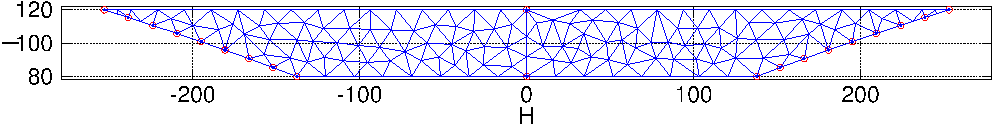
\includegraphics[width=\textwidth*7/8]{figures/domain_crop}
\caption{Example of domain within which the FPE is specified. A finite element triangulation of the domain is also shown.}
\label{F:domain}
\end{center}
\end{figure}

A set of illustrative values for $\mathring{\mathfrak a}$ is shown in Figures~\ref{F:a11_circ},~\ref{F:a12_circ} and~\ref{F:a22_circ}. Likewise, Figures~\ref{F:b1_circ} and~\ref{F:b2_circ} show values for $\mathring{\mathfrak b}$. Note that at points where no data is shown (ie. on the line $K=0$), the coefficients are unbounded, although certain coefficients do have a value in the limit $K \to 0$.

\begin{figure}
\begin{center}
\psfrag{a11*t}{$\mathring{\mathfrak a}_{11}$}
\psfrag{H}{$y_1$}
\psfrag{I}{$y_2$}
% 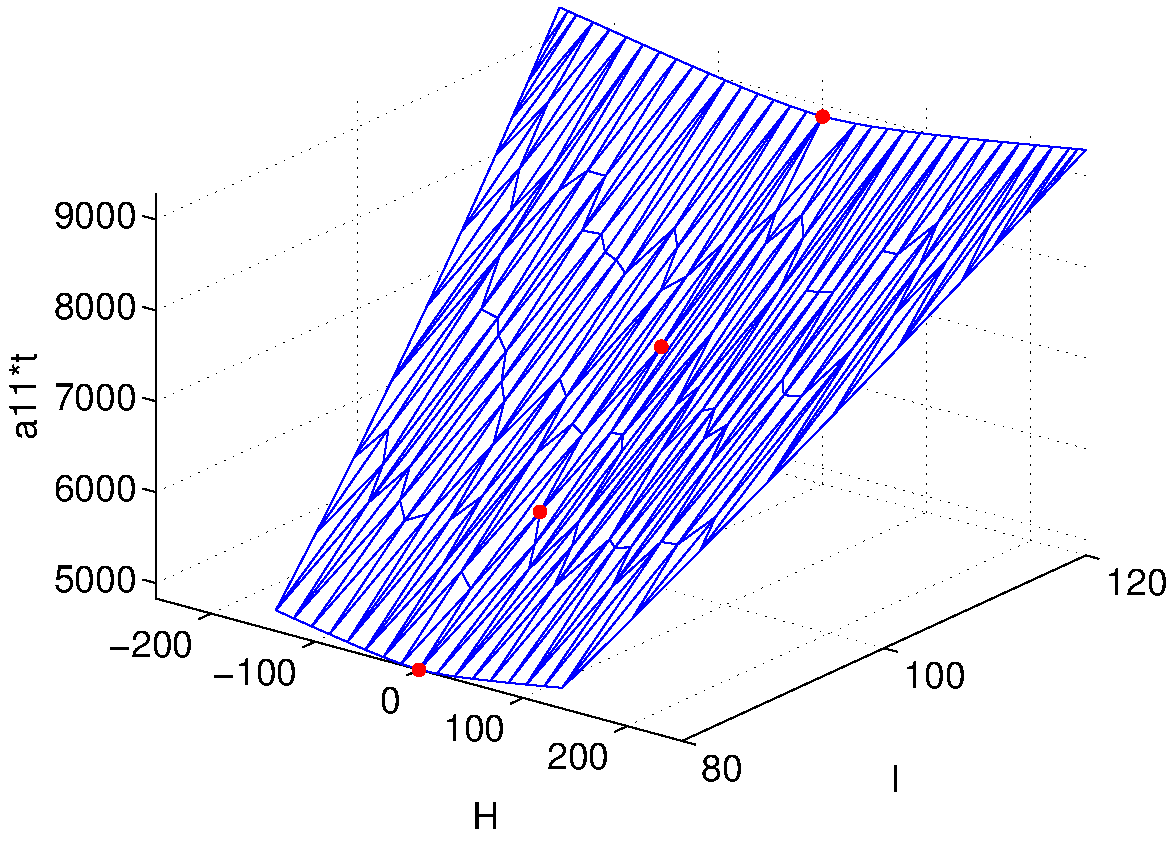
\includegraphics[clip=true,viewport=1in 1in 7in 5.5in,width=\textwidth*7/8]{figures/a11_circ}
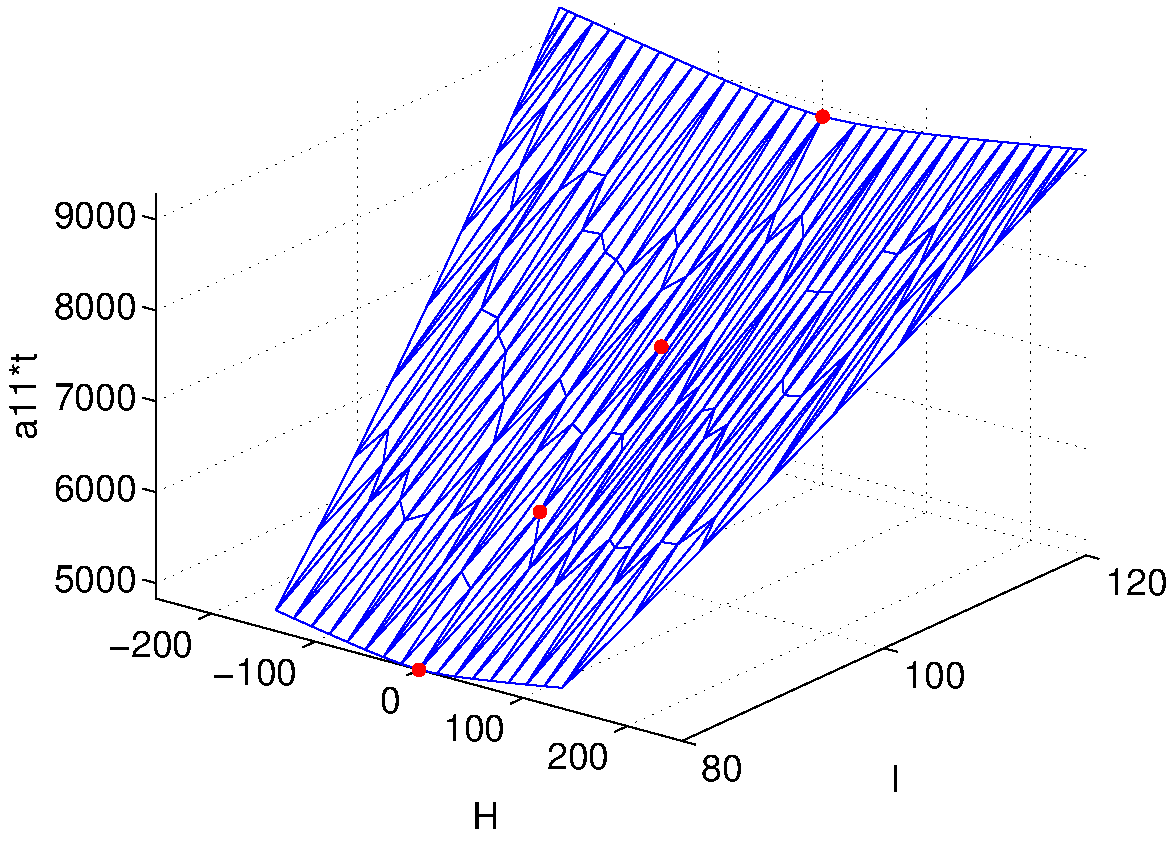
\includegraphics[width=\textwidth*7/8]{figures/a11_circ}
\caption{Example of numeric values for $\mathring{\mathfrak a}_{11}$. Circles denote points where the value is only defined by equation~\eqref{E:lim drift_11}.}
\label{F:a11_circ}
\end{center}
\end{figure}
\begin{figure}
\begin{center}
\psfrag{a12*t}{$\mathring{\mathfrak{a}}_{12}$}
\psfrag{H}{$y_1$}
\psfrag{I}{$y_2$}
% 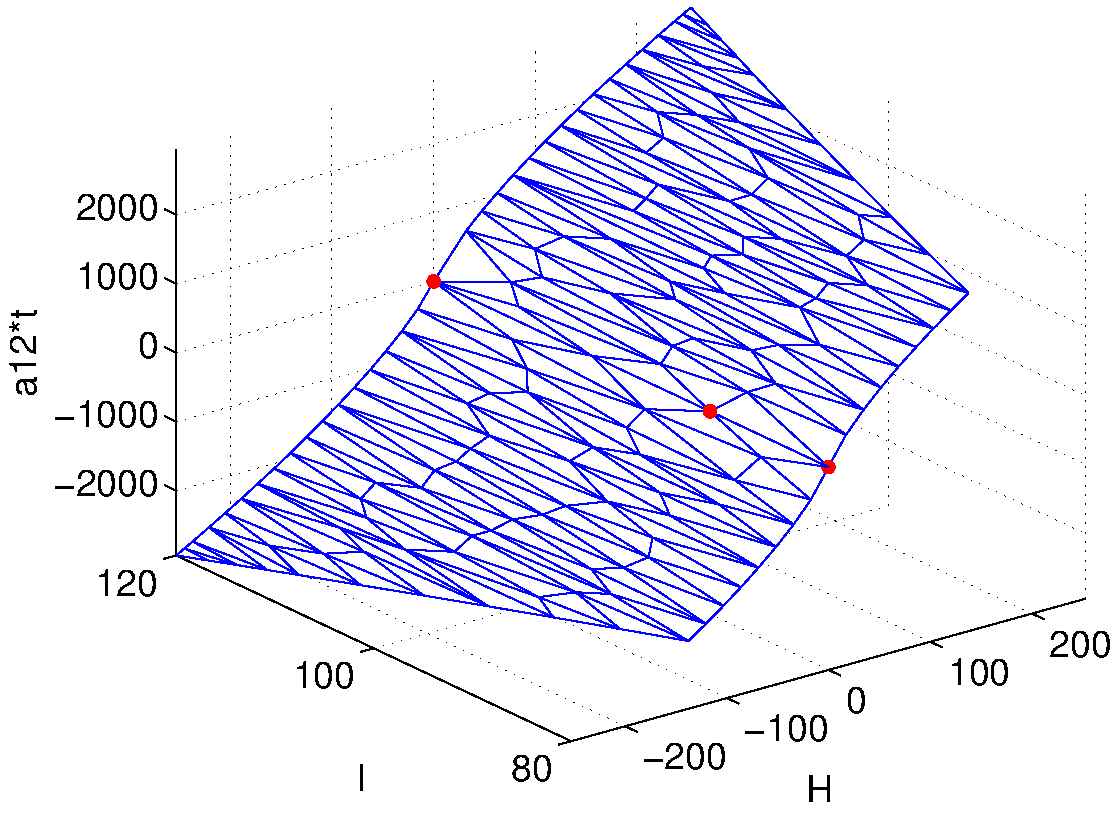
\includegraphics[clip=true,viewport=1in 1in 7in 5.5in,width=\textwidth*7/8]{figures/a12_circ}
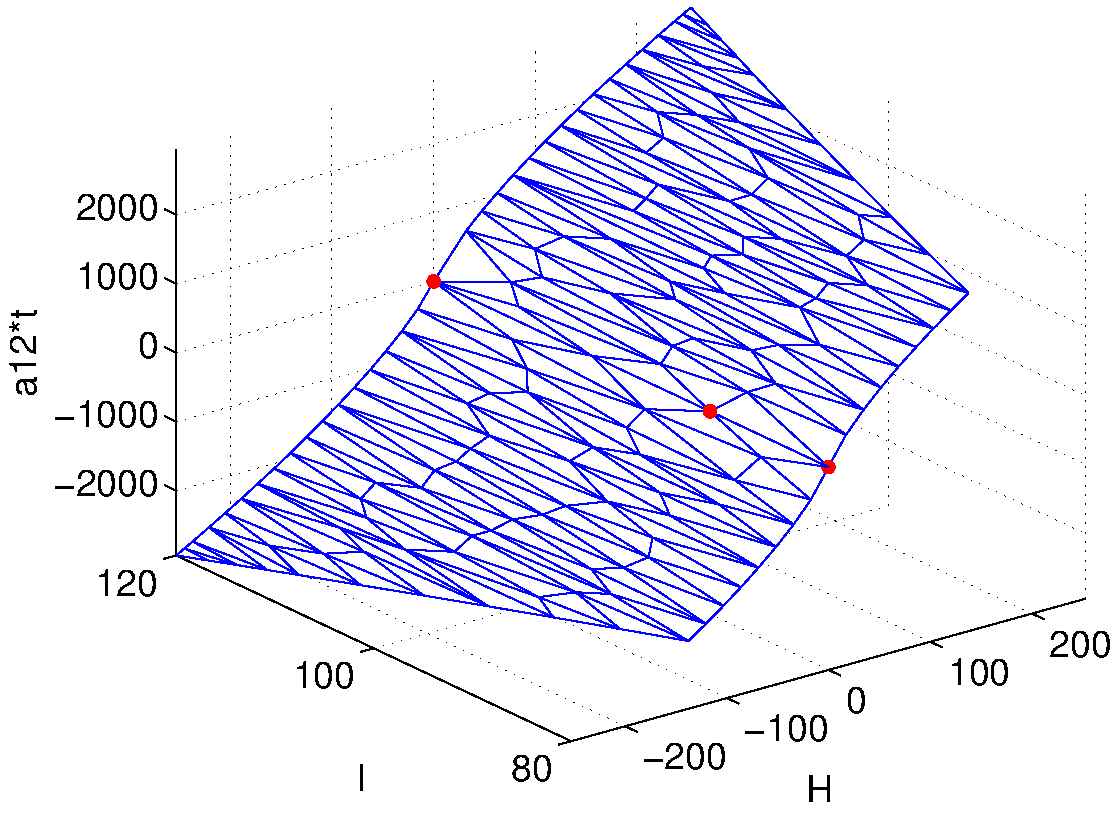
\includegraphics[width=\textwidth*7/8]{figures/a12_circ}
\caption{Example of numeric values for $\mathring{\mathfrak a}_{12}$. Circles denote points where the value is only defined by $\lim_{y_2 \to 0} \mathring{\mathfrak a}_{12} = 0$.}
\label{F:a12_circ}
\end{center}
\end{figure}
\begin{figure}
\begin{center}
\psfrag{a22*t}{$\mathring{\mathfrak{a}}_{22}$}
\psfrag{H}{$y_1$}
\psfrag{I}{$y_2$}
% 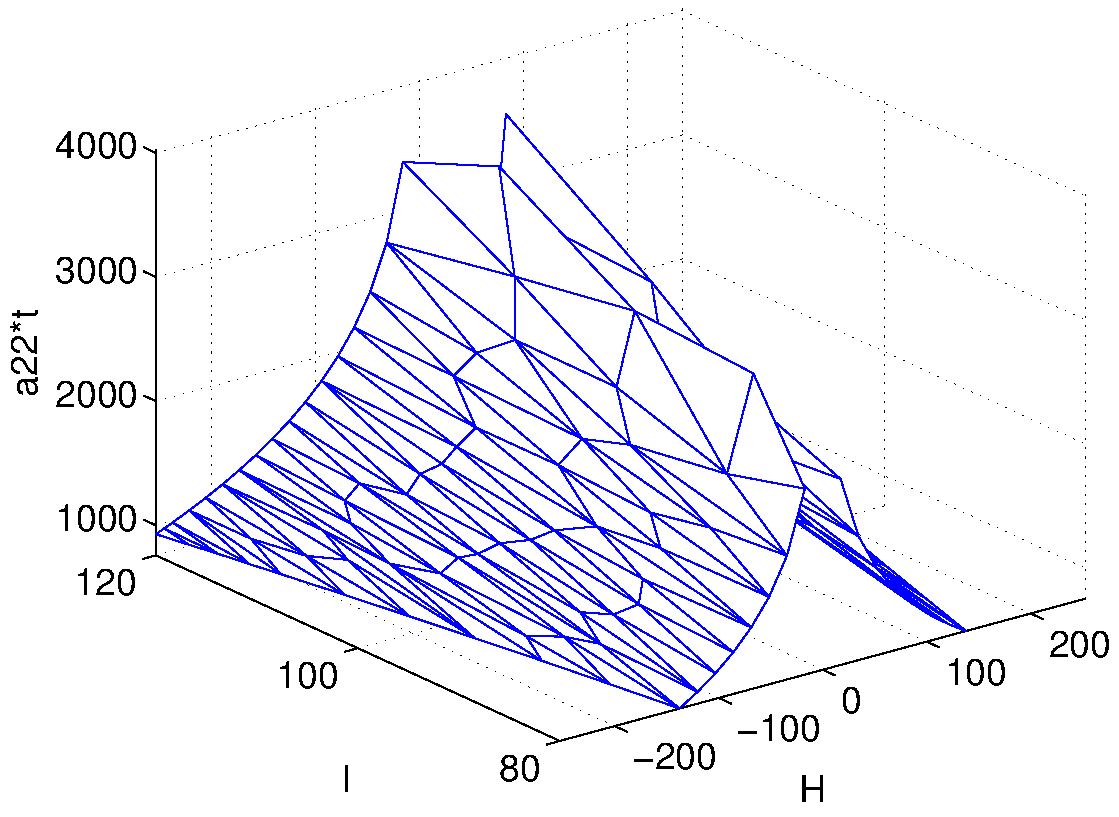
\includegraphics[clip=true,viewport=1in 1in 7in 5.5in,width=\textwidth*7/8]{figures/a22_circ}
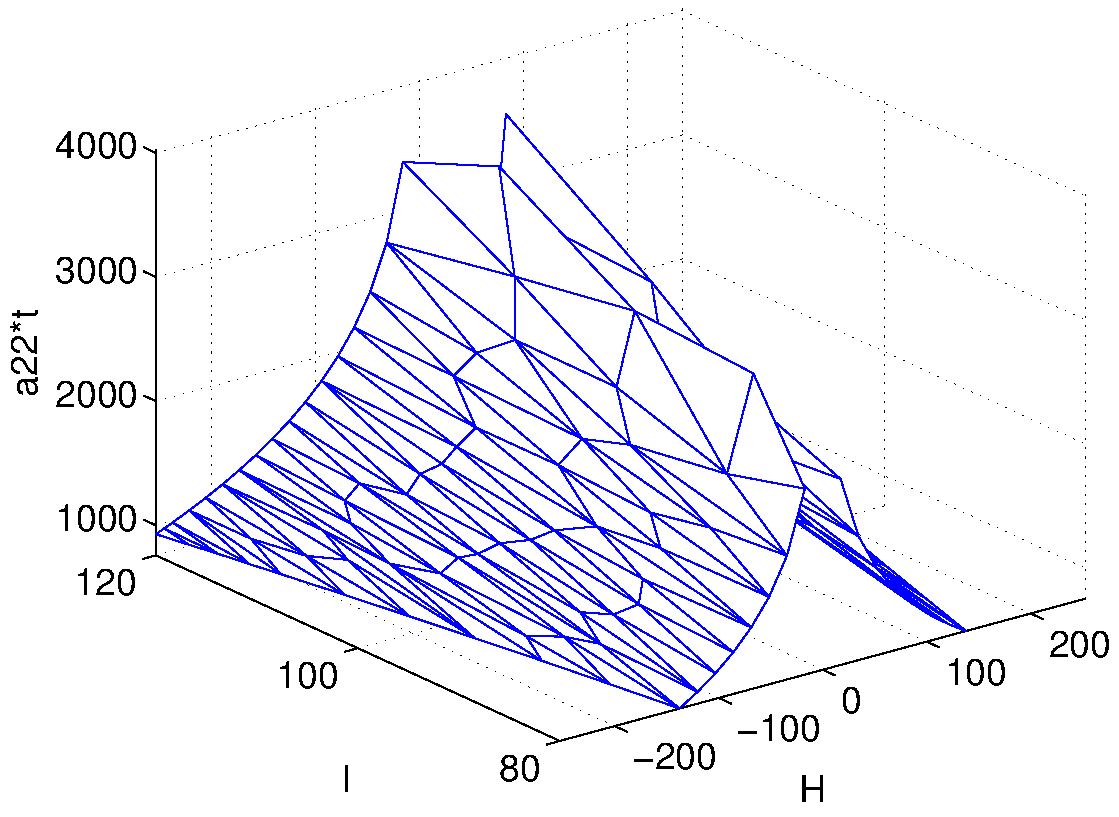
\includegraphics[width=\textwidth*7/8]{figures/a22_circ}
\caption{Example of numeric values for $\mathring{\mathfrak a}_{22}$. On the gluing edge, the value goes to infinity.}
\label{F:a22_circ}
\end{center}
\end{figure}
\begin{figure}
\begin{center}
\psfrag{b1*t}{$\mathring{\mathfrak{b}}_1$}
\psfrag{H}{$y_1$}
\psfrag{I}{$y_2$}
% 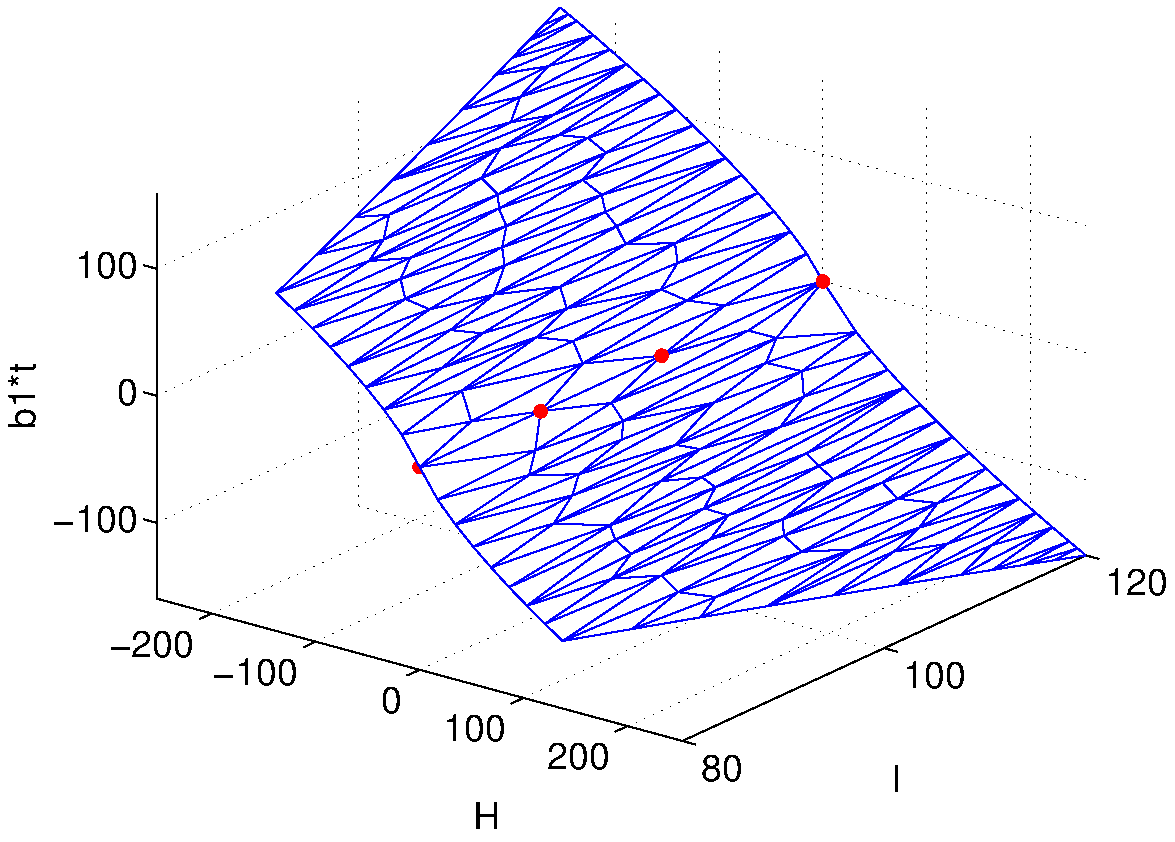
\includegraphics[clip=true,viewport=1in 1in 7in 5.5in,width=\textwidth*7/8]{figures/b1_circ}
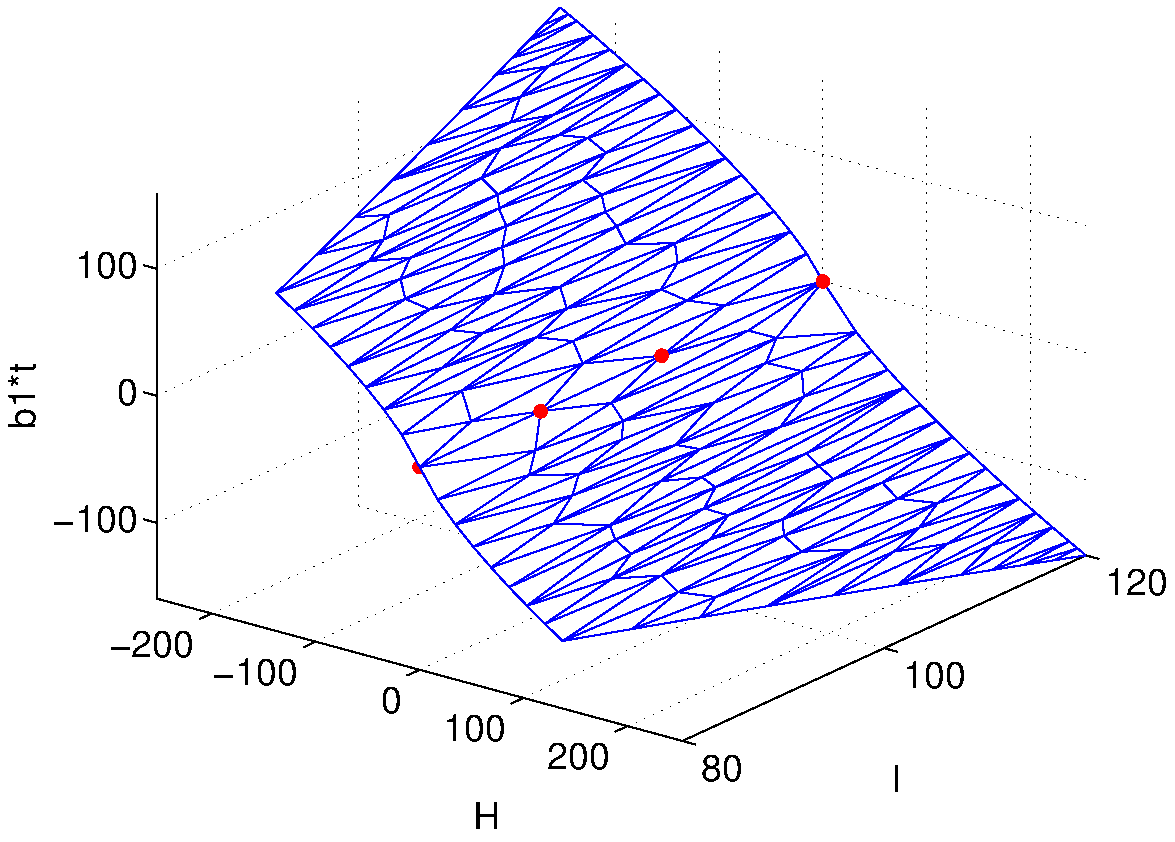
\includegraphics[width=\textwidth*7/8]{figures/b1_circ}
\caption{Example of numeric values for $\mathring{\mathfrak b}_1$. Circles denote points where the value is only defined by $\lim_{y_1 \to 0} \mathring{\mathfrak b}_1 = 0$.}
\label{F:b1_circ}
\end{center}
\end{figure}
\begin{figure}
\begin{center}
\psfrag{b2*t}{$\mathring{\mathfrak b}_2$}
\psfrag{H}{$y_1$}
\psfrag{I}{$y_2$}
% 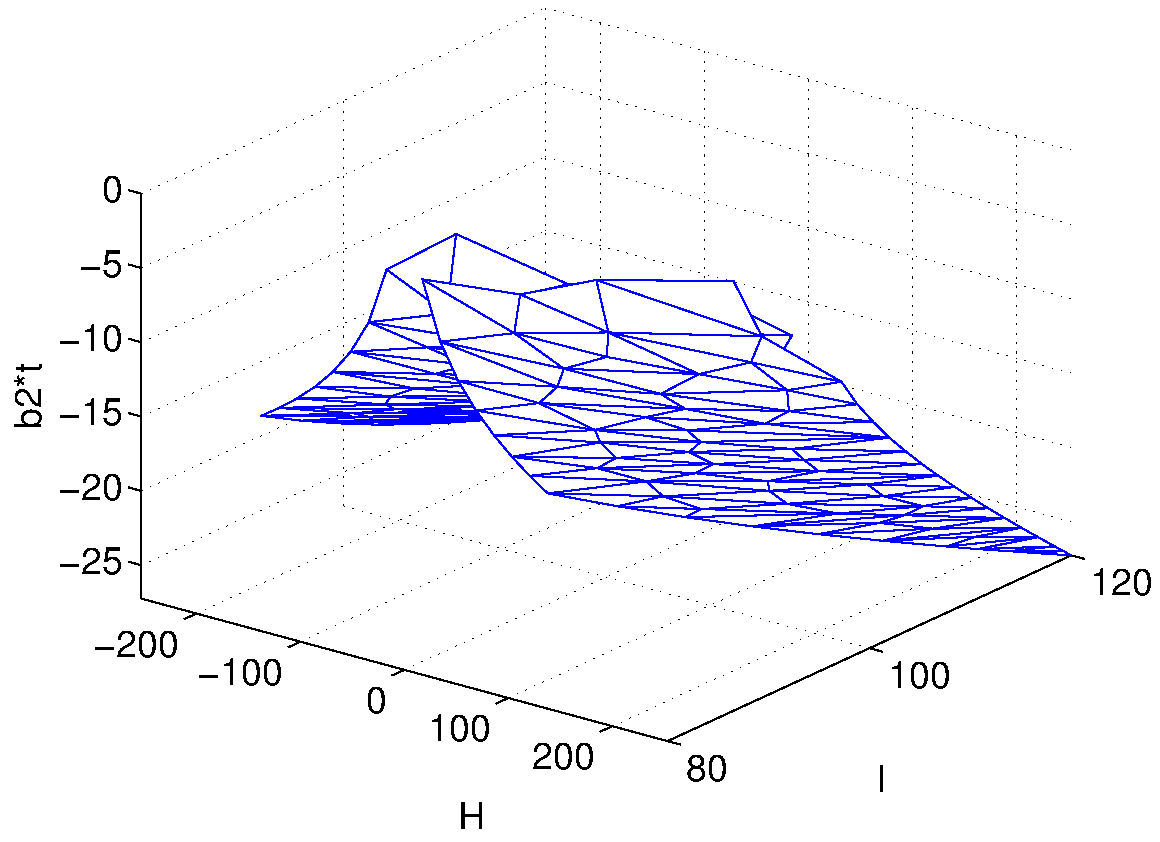
\includegraphics[clip=true,viewport=1in 1in 7in 5.5in,width=\textwidth*7/8]{figures/b2_circ}
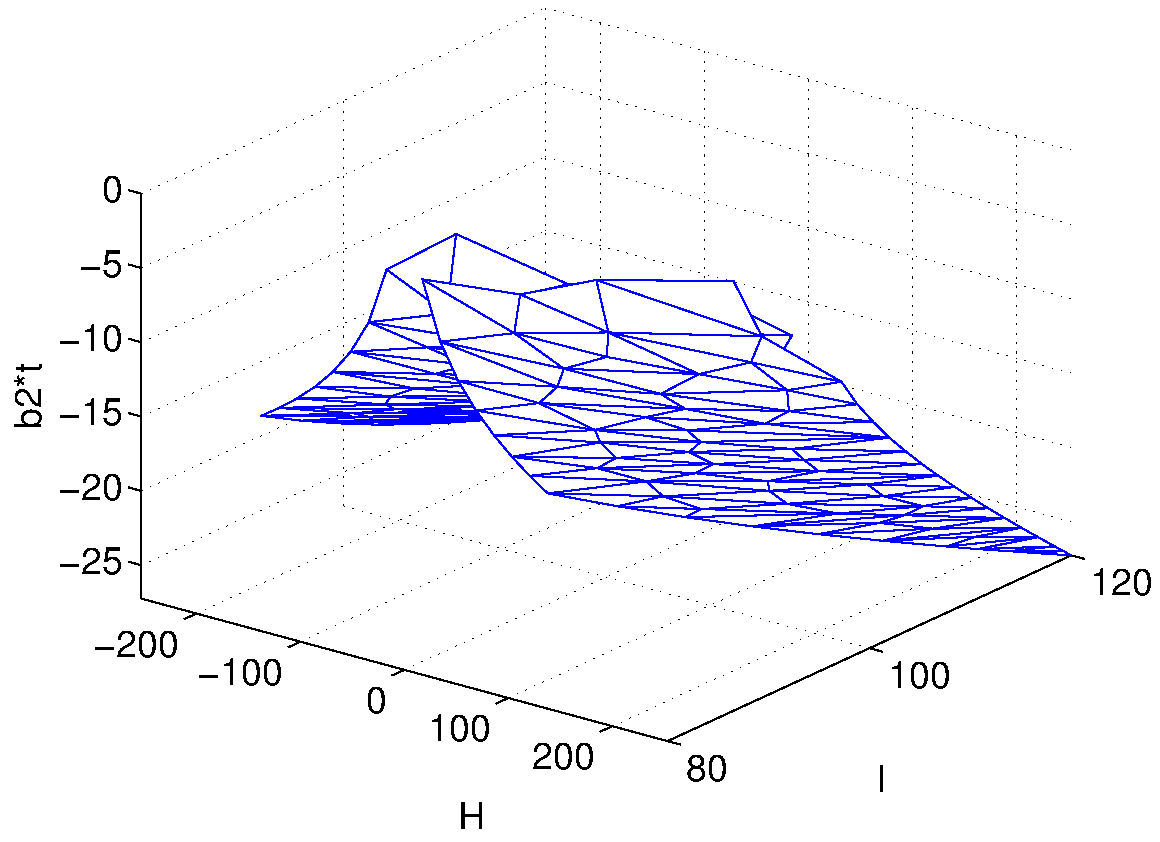
\includegraphics[width=\textwidth*7/8]{figures/b2_circ}
\caption{Example of numeric values for $\mathring{\mathfrak b}_2$. On the gluing edge, the value goes to infinity.}
\label{F:b2_circ}
\end{center}
\end{figure}

% FIXME Add figure showing the period

\section{Conclusions}

This chapter has shown how it is possible to analyze the stochastic motion of a pair of oscillators auto-parametrically coupled. In broad terms, the methodology used to achieve this was the same as for the wave model in \ref{c:sgwaves}. Differences exist in the details however. 1:2 resonance was imposed for the autoparametric problem whereas the wave model was near 1:1 resonance. The reduced domain of the autoparametric system contains two leaves, whereas the surface waves model has three. With regards to calculating averaged drift and diffusion coefficients, completely analytic results have been obtained for the autoparametric system, leading to formulas that contain elliptic integrals.

In the next chapter, the analysis of the autoparametric oscillator continues. Now that the generator of the reduced Markov process and its domain have been completely characterized in a weak sense, it becomes possible to derive a partial differential equation governing the evolution of probability density functions for the autoparametric oscillators. This equation will be derived in the next chapter, and it will be solved numerically.

%%% Local Variables: 
%%% mode: latex
%%% TeX-master: "main"
%%% End: 


\chapter{Probability Density Solutions}
\label{c:pdf}
\section{Introduction}

We turn our attention to producing solutions with the results of stochastic averaging theory. Specifically, stationary probability distribution functions are produced. First, the Fokker--Planck equation is derived. Then a finite element formulation of the Fokker--Planck problem is presented. Solutions for the surface gravity waves model and the autoparametric oscillator are then shown. Finally, the finite element results are validated with a sample path method.

\section{Derivation of the Fokker--Planck Equation}
% FIXME Inconsistent notation for p(y,t) (vs. p(t,y))
Before starting to derive the Fokker--Planck equation, it is necessary to consider how inner products behave under changes of variables. Specifically, it is found that if the area $A(y_1)$ is bounded by the curve $E(y_1)$, functions $f$ and $g$ satisfy $f(u_1,u_2,\psi,I) = f(y_1(u_1,u_2,I),y_2(u_1,u_2,I))$ and $g(u_1,u_2,\psi,I) = g(y_1(u_1,u_2,I),y_2(u_1,u_2,I))$, then
\begin{multline*}
\int_{A(y_1)} f(u_1,u_2,\psi,I) g(u_1,u_2,\psi,I) du_1 du_2 d\psi dI\\
= \int f(y_1,y_2) g(y_1, y_2) \period(y_1,y_2) dy_1 dy_2.
\end{multline*}
To show this, the first step is to change the variables of integration of the integral on the left hand of the equation above. This yields
\begin{equation}
\label{e:KLISmL}
\int_{A(y_1)} f(u_1,u_2,\psi,I) g(u_1,u_2,\psi,I) \left\lvert\frac{\partial u_1}{\partial y_1}\right\rvert dy_1 du_2 d\psi dy_2.
\end{equation}
Denoting arc length along a Hamiltonian orbit $E(y_1)$ by $s$, since
\[
\frac{ds}{du_2} = \frac{\lVert \nabla y_1 \rVert}{\lvert dy_1/du_1\rvert}
\]
Equation \eqref{e:KLISmL} can be written as
\[
\int \oint_{E(y_1)} \frac{f(u_1,u_2,\psi,I) g(u_1,u_2,\psi,I)}{\lVert \nabla y_1 \rVert} ds dy_1 d\psi dy_2.
\]
After substituting the assumed functional form of $f$ and $g$, it follows that the inner product is given by
\[
\left\langle f(y), g(y) \right\rangle_{K,I} \equiv \int_{K=y_1} \int_{I=y_2} f(y) g(y) \period (y) dy_1 dy_2
\]

Now we derive the Fokker-Planck equation (FPE) for the density of $\{(k_t, I_t); t \ge 0\}$. We present a rigorous derivation that takes care of the killed process at $I^*$ and examine the stationary behavior of the FPE when $I^*= \infty$. We assume that there is a $p\in C^\infty((0,\infty)\times \bigcup_{i=1}^n \Gamma_i )$ and a $p_{i}^\BDY\in C^\infty((0,\infty))$ such that for any $f\in \mathscr{D}_\Graph^\dag$
\begin{multline}
\label{E:expectation}
\Expectation^\epsilon_x \left[f(k_t, I_t) \right] = \sum_{i=1}^n (\pm) \int_{\Gamma_i} f_i(y) p_i(y,t) \period_i(y) dk dI\\
+ \sum_{i=1}^n (\pm) \int_{k^i} f_i(k,I^*) \period_{i}(k,I^*) p_i^\BDY(k,t) dk
\end{multline}
where the `$+$' sign is taken on the leaves where the coordinate $k$ is greater than $K({\Order})$ and the `$-$' sign is taken on the leaves where the coordinate $k$ is less than $K({\Order})$.) $p_i(y,t)$ and $p_{i}^\BDY(t)$ are the density of the law of $(k_t, I_t)$ relative to Lebesgue measure on $\bigcup_{i=1}^n \Gamma_i$ and a Dirac mass at $I^*$. Since we kill $(k_t, I_t)$ at $I^*$, mass may accumulate there, necessitating a Dirac measure at $I^*$.
Differentiating~\eqref{E:expectation} with respect to time yields
\begin{multline}
\label{E:exp-prime}
\frac{\partial}{\partial t} \Expectation^\epsilon_x\left[ f(k_t, I_t) \right] = \sum_{i=1}^n (\pm) \int_{\Gamma_i} f_i(y) \frac{\partial p_i}{\partial t}(t,y) \period_i(y) dk dI\\
+ \sum_{i=1}^n (\pm) \int_{k_i} f_{i}(k,\,I^*) \period_{i}(k,I^*)  \frac{\partial p_i^\BDY}{\partial t}(k,t) dk
\end{multline}
On the other hand
\begin{equation}
\begin{aligned}
\frac{\partial}{\partial t} \Expectation^\epsilon_x\left[f(k_t ,I_t) \right] &= \Expectation^\epsilon_x\left[(\gen^\dagger_i f)(k_t, I_t) \right]\\
&= \sum_{i=1}^n (\pm) \int_{\Gamma_i} (\gen^\dagger_i f_{i})(y) p_{i}(t,y) \period_{i}(y) dk dI\\
&\quad + \sum_{i=1}^n (\pm) \int_{0}^{k_{i}^{c}(I^*)}\!\! (\gen^\dagger_i f_i)(k,I^*) \period_i(k,I^*) p_{i}^\BDY(k,t) dk
\end{aligned}
\label{E:exp-ito}
\end{equation}
Combining Equations \eqref{E:exp-prime} and \eqref{E:exp-ito} gives
\begin{multline}
\sum_{i=1}^n (\pm) \int_{0}^{k_{i}^{c}(I^*)} \left\{f_i(k,I^*) \frac{\partial p_i^\BDY}{\partial t}(t,k) - (\gen^\dagger_i f_i)(k,I^*) p_i^\BDY(t,k) \right\} \period_{i}(k,I^*) dk\\
+ \sum_{i=1}^n (\pm) \int_{\Gamma_i} \left\{f_i(y) \frac{\partial p_i}{\partial t}(t,y) - (\gen^\dagger_i f_i)(y) p_{i}(t,y) \right\} \period_i(y) dk dI = 0
\label{E:step0}
\end{multline}

\begin{remark}
\emph{Relation between the gluing condition and the probability flux condition.}
The gluing condition and the probability flux condition are related. This is seen by starting with the generic ``adjoint'' formula for a linear second order operator $\gen$ and its adjoint $\gen^\text{adj}$. Referring to, for example \citet[\S3.6]{zauderer98:_partial_differ_equat_of_applied_mathem}, on adjoint differential operators, the divergence theorem gives
\[
\int_G \{p \gen f - f \gen^{\text{adj}} p \}dv = \int_{\partial G} \boldsymbol{P}\cdot\boldsymbol{n} ds.
\]
When the generator has the form given in Definition \ref{d:reduced generator},
\[
P_j^i = \frac12 \sum_{k=1}^2 \mathring{\Aa}^i_{jk} \frac{\partial f_{i}(y)}{\partial y_k} p_i(t,y) + f_i J_j^i
\]
Referring to~\eqref{E:dom-graph}, the first term in the sum is
recognized as being associated with the gluing condition while the
second is associated with the probability flux condition. The probability flux on leaf $i$ in the direction $y_j$ is:
\begin{equation}
\label{E:prob flux}
J_j^i(t,y) \equiv \mathring{\mathfrak{b}}_{j}^{i}(y) p_{i}(t,y) - \frac12 \sum_{k=1}^2 \frac{\partial}{\partial y_k} \left(
\mathring{\Aa}_{jk}^i(y) p_i(t,y)\right)
\end{equation}
\end{remark}

Applying the divergence theorem to the last term on the left side of~\eqref{E:step0} and making use of the properties of $\mathscr{D}_\Graph^\dag$ yields
\begin{multline}
\sum_{i=1}^n (\pm) \int_{\Gamma_i} \left\{ \frac{\partial p_{i}}{\partial t}(t,y) - \gen^{\dagger,\text{adj}}_{i} p_{i} (t,y) \right\} f_{i}(y) \period_{i}(y) dk dI\\
+ \sum_{i=1}^n (\pm) \int_{0}^{k_{i}^{c}(I^*)} f_{i}(k,\,I^*) \frac{\partial p_i^\BDY}{\partial t}(t,k) dk\\
= \sum_{i=1}^n(\pm) \int_{\partial\Gamma_i} \sum_{j=1}^2 J_j^i(t,y) f_i(y) \cdot \nu_j ds\\
+ \sum_{i=1}^n (\pm) \int_{\partial\Gamma_i} \frac12 \sum_{j=1}^2 \left\{\sum_{k=1}^2 \mathring{\Aa}_{jk}^i(y) \frac{\partial f_{i}}{\partial y_k}(y)\right\} p_{i}(t,y) \cdot \nu_j ds
\label{E:step6}
\end{multline}
where
\[
\gen^{\dagger,\text{adj}}_i = \frac{1}{\period_i(y)} \sum_{j=1}^2 \frac{\partial}{\partial y_j}(\mathring{\mathfrak b}_j(y) p(y)) - \frac{1}{2 \period_i(y)} \sum_{j,k=1}^2 \frac{\partial^2}{\partial y_j \partial y_k} (\mathring{\mathfrak a}_{jk}(y) p(y)).
\]

For the autoparametric problem, each $\partial\Gamma_i$ consists of a vertical line ($\nu_2=0$) representing the vertex ${\Order}\equiv[0,I^*]$, a horizontal ($\nu_1=0$) line ${\bigb}\equiv[0,{k_i^c(I^*)}]$, at which the process is killed ($I=I^*$), and a curved line ${\bigc_i}\equiv \{(k,I)\in \reals^2: k= (-1)^iI\sqrt{3I}/9\}$, for $i=1,2$ representing the fixed points. Hence, by explicitly expressing the boundary $\partial\Gamma_i$, equation~\eqref{E:step6} can be rewritten as
\begin{multline}
\sum_{i=1}^n (\pm) \int_{\Gamma_i} \left\{\frac{\partial p_i}{\partial t}(t,y) - \mathring \gen^{\dagger,\text{adj}}_{i} p_{i} (t,y) \right\} f_i(y) \period_{i}(y) dk dI\\
+ \sum_{i=1}^n (\pm) \int_{\bigb} \left[\frac{\partial p_i^\BDY}{\partial t}(t,\,k) - J_2^{i}(t,k,I^*) \right] f_i(k,I^*) dk\\
= \sum_{i=1}^n \int_{\bigc_i} \sum_{j=1}^2 J_j^i(t,y) f_i(y) \cdot \nu_j ds + \sum_{i=1}^n (\pm) \int_{\Order} J_1^i(t,\Order,I) f_i(\Order,I) dI\\
+ \frac12 \sum_{i=1}^n (\pm) \int_{\bigb} \left\{\sum_{k=1}^2 \mathring{\Aa}_{2k}^i(k,I^*) \frac{\partial f_i}{\partial y_k}(k,I^*)\right\}\, p_i(t, k, I^*) dk\\
+ \frac12 \int_{\bigc} \sum_{j=1}^2 \left\{\sum_{k=1}^n \mathring{\Aa}_{jk}^i(y) \frac{\partial f_i}{\partial y_k}(y)\right\} p_{i}(t,y) \cdot \nu_j ds\\
+ \frac12 \sum_{i=1}^n (\pm) \int_{\Order} \left\{ \sum_{k=1}^2 \mathring{\Aa}_{1k}^i(\Order,I)
\frac{\partial f_i}{\partial y_k}(\Order,I)\right\} p_i(t,\Order,I) dI
\label{E:step7}
\end{multline}
The properties of $f_i$ defined for the limiting domain $\mathscr{D}_\Graph^\dag$ (i.e. equation~\eqref{E:dom-graph-simplified}) will not eliminate any other terms in~\eqref{E:step7}. Boundary conditions for $p_i$ are derived from the right hand side of~\eqref{E:step7}. Along $\bigc_i$, which represent regular elliptic fixed points~(non-degenerate), we impose the zero probability flux boundary condition. Hence the first term in the right hand side of~\eqref{E:step7} becomes identically zero. Once again for $f_i \in \mathscr{D}_\Graph^\dag$, the second and the last term vanish by imposing zero net flux and continuity of probability density at the vertex ${\Order}$, respectively.
% Since $h_i^c, i=1,2$ are the energy associated with regular elliptic fixed points~(non-degenerate)
% FIXME Reference given here Lemma~\ref{L:fsmoothness} in \cite{namachchivaya01:_non_duffin_pol}
% \[
% \lim_{z \searrow h_{i}^{c}} \mathring\Aa_{jk}^{i}(z)=0, \quad \lim_{z \searrow h_{i}^{c}} \frac{\partial f_{i}}{\partial z_k}(z) \;\; \text{are finite}, \quad \lim_{z \searrow h_{i}^{c}} p_{i} (t,z) \;\; \text{are normalizable}
% \]
% Hence, the fourth term on the right hand side of~\eqref{E:step7} and the third term on the right hand side vanishes in the above expression due to the fact the process is killed when the energy reaches $I^*$.

Hence $p_i$ satisfies
\begin{enumerate}
\item the FPE,
\begin{equation}
\frac{\partial p_i}{\partial t}(t,y) = \gen^{\dagger,\text{adj}}_i p_i(t,y) \; \text{ for } t > 0 \text{ and } y \in \Gamma_i
\label{E: FPE time-dependent}
\end{equation}

\item conservation of probability flux at the vertex $\mathcal{O}$
\begin{equation}
\lim_{y \to \mathcal O} \sum_{i = 1}^N J^i(t,y) \cdot \nu^i = 0
\label{E:cpfc}
\end{equation}

\item the zero probability flux condition along the edges identified with elliptic fixed points,
\begin{equation}
\eval{\sum_{j=1}^2 \left(\mathfrak b_j^i(y) p_i(t,y) - \frac12 \sum_{k=1}^2 \frac{\partial}{\partial y_k} \left(\Aa_{jk}^i(y)\,p_{i}(t,y)\right)\right) \cdot \nu_j}_{y = \bigc_i} = 0
\label{E:BC elliptic}
\end{equation}
\item killing of the process when the energy reaches $I^*$, i.e.,
\begin{equation}
\lim_{y_2 \to I^*} p_i(t,y) = 0.
\label{E:BC upper}
\end{equation}
\end{enumerate}
The dynamics of $p_i^\BDY$ are defined by
\[
\frac{\partial p_{i}^\BDY}{\partial t}(t,k) = \mathring{\mathfrak{b}}_2^{i}(y)\,p_i(t,k,I^*) - \frac12 \sum_{k=1}^2
\frac{\partial}{\partial y_k} \left(\mathring\Aa_{2k}^i(z) p_i(t,k,I^*)\right)
\]
i.e., the rate of change of probability in the cemetery state $I^*$, on each leg of the graph, is equal to the flux entering $I^*$ from the interior.

\section{Finite Element Solution to the Fokker-Planck Equation}

We solve the FPE at steady-state. Based on equation~\eqref{E: FPE time-dependent}, within leaves where the FPE is specified we have:
\begin{equation}
\label{E:FPE}
\sum_{j=1}^2 \frac{\partial}{\partial y_j}(\mathring{\mathfrak b}_j(y) p(y)) - \frac12 \sum_{j,k=1}^2 \frac{\partial^2}{\partial y_j \partial y_k} (\mathring{\mathfrak a}_{jk}(y) p(y)) = 0
\end{equation}

The boundary condition given in equation~\eqref{E:BC elliptic} cannot be imposed directly because it uses coefficients divided by the period, whereas the FPE contains ``ringed'' (i.e. not divided by the period) coefficients. Applying the chain and the product rule for differentiation, equation \eqref{E:BC elliptic} on either leaf becomes
\begin{multline}
\frac{1}{\period(y)} \sum_{j=1}^2 \Bigg(\mathring{\mathfrak{b}}_j(y) p(y) - \frac12 \sum_{k=1}^2 \Big[\frac{\partial}{\partial y_k} (\mathring{\mathfrak{a}}_{jk}(y) p(y)) - \frac{\mathring{\mathfrak{a}}_{jk} p(y)}{\period(y)} \frac{\partial \period(y)}{\partial y_k}\Big]\Bigg) \nu_j \Bigg\rvert_{y = \bigc} = 0\\
\frac{1}{\period(y)} \sum_{j=1}^2 \Bigg(J_j(y) + \frac12 \sum_{k=1}^2 \frac{\mathring{\mathfrak{a}}_{jk} p(y)}{\period(y)} \frac{\partial \period(y)}{\partial y_k}\Bigg) \nu_j \Bigg\rvert_{z = \bigc} = 0
\label{E:BC elliptic 2}
\end{multline}

At the ``upper'' boundary, $I = I^*$, the boundary condition given in equation~\eqref{E:BC upper} should be imposed. This introduces a difficulty however since equation~\eqref{E:BC upper} is formally derived in the limit $I^* \to \infty$. Since representing this limit in numerical calculations may not be straightforward, we choose to simplify the situation by imposing a condition like the zero probability flux in equation~\eqref{E:BC elliptic} instead. In our results, we will need to ensure that the finite value selected for $I^*$ is sufficiently large.

As can be seen in Figure~\ref{F:domain}, the domain used with the finite-element approach does not start at $I=0$, this is to avoid the cusp at the origin. As a result, a boundary condition must be imposed on that boundary. As with the boundary at $I^*$, the zero-flux boundary condition will be imposed.

Finally the conservation of probability flux condition, in equation~\eqref{E:cpfc}, needs to be considered. As shown in Appendix~\ref{A:gluing BC simplification}, it can be demonstrated numerically that this condition simplifies to:
\begin{equation}
\eval{\frac{\partial p_1}{\partial k}}_{z = \mathcal{O}} = \eval{\frac{\partial p_2}{\partial k}}_{z = \mathcal{O}}
\label{E:cpfc simplified}
\end{equation}

\subsection{Weak Formulation of the Fokker-Planck Problem}

Use of the finite element method entails specifying a weak form of the Fokker-Planck problem. The weak formulation of the FPE given here is adapted from \citet{langtangen91:_fokker_planck}, where a method to obtain steady-state solutions using a finite-element approach is presented. The use of Langtangen's method is necessary because the steady-state FPE is satisfied by the trivial solution, $p=0$. Langtangen's method enforce the normalization condition and thus provides a nontrivial solution.
% Give alternatives to Langtangen's method: (i) fix PDF at some point in the domain, (ii) time-dependent FPE solution.
Essentially, our task consists of extending Langtangen's method to multi-leaf domains (i.e. with a conservation of probability flux condition.)

To begin, we introduce a Hilbert space, $H^1$, that we will use to specify weak solutions. Let
\begin{align}
V &= \left\{v \in H^1(\mathfrak I): \int_\mathfrak I v dz = 1\right\} &\text{and}&& W &= \left\{v \in H^1(\mathfrak I): \int_\mathfrak I v dz = 0\right\}
\label{E:weak spaces}
\end{align}
% FIXME Change notation: \mathfrak{I} -> \Gamma
Note that the definitions above do not reflect that we have two leaves, $\mathfrak{I}_{1,2}$ -- we start our presentation by considering the simpler case where the domain of the FPE is a single leaf. The next step is to derive a bilinear form corresponding to the FPE. The weak form of the steady-state FPE, equation~\eqref{E:FPE}, is
\[
\int_\mathfrak I \phi (\nabla \cdot J) dy = 0
\]
where $\phi \in W$ and the $p \in V$ (recall from equation~\eqref{E:prob flux} that $p$ is contained within $J$.) Integration by parts gives
\[
-\int_\mathfrak I \nabla \phi \cdot J dy + \int_{\partial \mathfrak I} \phi J \cdot \nu d\sigma(y) = 0
\]
Separating $\partial \mathfrak I$ into an exterior boundary and an interior boundary (i.e. the gluing edge),
\begin{equation}
-\int_\mathfrak I \nabla \phi \cdot J dy + \int_{\partial \mathfrak I_\bigc} \phi J \cdot \nu d\sigma(y) + \int_{\partial \mathfrak I_\mathcal{O}} \phi J \cdot \nu d\sigma(y) = 0
\label{E:FPE weak}
\end{equation}
On $\partial \mathfrak I_\bigc$, using equation~\eqref{E:BC elliptic 2} gives
\[
J \cdot \nu = -\frac{1}{2 \period(y)} \sum_{j,k=1}^2 \mathring{\mathfrak{a}}_{jk} \frac{\partial \period(y)}{\partial y_k} \nu_j p(y)
\]
Thus equation~\eqref{E:FPE weak} becomes
\begin{equation}
\int_\mathfrak I \nabla \phi \cdot J dy + \int_{\partial \mathfrak I_\bigc} \frac{\phi}{2 \period(y)} \sum_{j,k=1}^2 \mathring{\mathfrak{a}}_{jk} \frac{\partial \period(y)}{\partial y_k} \nu_j p(y) d\sigma(y) + \int_{\partial \mathfrak I_\mathcal{O}} \phi J \cdot \nu d\sigma(y) = 0
\label{E:FPE weak 2}
\end{equation}
Now the finite-element problem is formulated so as to treat both leaves together. In so doing, we must redefine the quantities given in~\eqref{E:weak spaces}, we have
\begin{align*}
V &= \left\{v \in H^1(\mathfrak I_1 \cup \mathfrak I_2): \int_\mathfrak{I_1} v dy + \int_\mathfrak{I_2} v dy = 1\right\}\\
W &= \left\{v \in H^1(\mathfrak I_1 \cup \mathfrak I_2): \int_\mathfrak{I_1} v dy + \int_\mathfrak{I_2} v dy = 0\right\}
\end{align*}
and~\eqref{E:FPE weak 2} and the results of Appendix~\ref{A:gluing BC simplification} on simplifications of the conservation of probability flux condition give
\begin{multline*}
\int_{\mathfrak I_1} \nabla \phi \cdot J^1 dy + \int_{\partial \mathfrak I_{\bigc_1}} \frac{\phi}{2 \period(y)} \sum_{j,k=1}^2 \mathring{\mathfrak{a}}_{jk}^1 \frac{\partial \period(y)}{\partial y_k} \nu_j^1 p_1(y) d\sigma(y)\\
+ \int_{\mathfrak I_2} \nabla \phi \cdot J^2 dy + \int_{\partial \mathfrak I_{\bigc_2}} \frac{\phi}{2 \period(y)} \sum_{j,k=1}^2 \mathring{\mathfrak{a}}_{jk}^2 \frac{\partial \period(y)}{\partial y_k} \nu_j^2 p_2(y) d\sigma(y) = 0
\end{multline*}
% FIXME Explain that can essentially ignore gluing BC, but in evaluating coefficients, need to place quadrature points away from gluing edge since certain coefficients are infinite there.
Since on the edge $\partial \mathfrak I_\mathcal{O}$ equation~\eqref{E:cpfc simplified} holds and $\mathring{\mathfrak{a}}_{11}^1 = \mathring{\mathfrak{a}}_{11}^2$, the equation above gives the bilinear form we sought:
\begin{multline}
\label{E:weak FPE}
L(p,\phi) = \int_{\mathfrak I_1} \nabla \phi \cdot J^1 dy + \int_{\partial \mathfrak I_{\bigc_1}} \frac{\phi}{2 \period(y)} \sum_{j,k=1}^2 \mathring{\mathfrak{a}}_{jk}^1 \frac{\partial \period(y)}{\partial y_k} \nu_j^1 p_1(y) d\sigma(y)\\
+ \int_{\mathfrak I_2} \nabla \phi \cdot J^2 dy + \int_{\partial \mathfrak I_{\bigc_2}} \frac{\phi}{2 \period(y)} \sum_{j,k=1}^2 \mathring{\mathfrak{a}}_{jk}^2 \frac{\partial \period(y)}{\partial y_k} \nu_j^2 p_2(y) d\sigma(y)
\end{multline}
Note that the bilinear form is non-symmetric.

We wish to solve
\begin{align}
\label{E:weak FPE 2}
L(p,\phi) &= 0, & \phi &= v - p, \forall \, v \in V.
\end{align}
The discrete version of \eqref{E:weak FPE} is found with the approximation
\[
p(y) \approx p^h(y) = \sum_{j=1}^n H_j(y) p_j
\]
where $H_j(x)$ denote finite-element shape functions. The discrete form of the normalization condition is
\[
\int_{\mathfrak I_1} p^h(y) dy + \int_{\mathfrak I_2} p^h(y) dy = 1
\]
which can be written
\[
c^T p = 1
\]
where $c = (c_1, c_2, \dots, c_n)$ and
\[
c_i = \int_{\mathfrak I_1} H_i(y) dy + \int_{\mathfrak I_2} H_i(y) dy.
\]
The discrete equivalent to~\eqref{E:weak FPE 2} is
\begin{align}
L(p^h,\phi^h) &= 0, & \phi^h &= v^h - p^h, \forall \, v^h \in V^h.
\label{E:FPE FEM}
\end{align}
Here, $\phi \in W^h$ and
\begin{multline*}
V^h = \Big\{v = \sum_{j=1}^n H_j(y) v_j, v_j \in \reals, H_j \in H^1(\mathfrak I_1 \cup \mathfrak I_2), j = 1,\dots,n:\\
\sum_{j=1}^n c_j v_j = 1\Big\}
\end{multline*}
\begin{multline*}
W^h = \Big\{v = \sum_{j=1}^n H_j(y) v_j, v_j \in \reals, H_j \in H^1(\mathfrak I_1 \cup \mathfrak I_2), j = 1,\dots,n:\\
\sum_{j=1}^n c_j v_j = 0\Big\}
\end{multline*}
Typical finite-element problems have weighting functions equal to shape functions, but this is not possible for the Fokker-Planck equation since $H_i \notin W^h$. Define
\[
U = \left\{q = (q_1,\dots,q_n)^T \in \reals^n: c^T q = 0.\right\}.
\]
Then one can construct $\phi^h \in W^h$:
\[
\phi^h = \sum_{i=1}^n q_i H_x(x), \quad q \in U.
\]
Equation~\eqref{E:FPE FEM} then results in the following system of algebraic equations for $p$:
\begin{align*}
q^T K p &= 0, & \forall& q \in U\\
c^T p &= 1
\end{align*}
The specific form of $K$ is:
\begin{align*}
K_{ij} &= \int_\Omega \frac{\partial \phi_i}{\partial y_1} \Big[\Big\{-\mathring{\mathfrak b}_1 + \frac12 \Big(\frac{\partial \mathring{\mathfrak a}_{11}}{\partial y_1} + \frac{\partial \mathring{\mathfrak a}_{12}}{\partial y_2}\Big)\Big\}\phi_j\\
&\quad + \frac12 \Big(\mathring{\mathfrak a}_{11}\frac{\partial \phi_j}{\partial y_1} +
\mathring{\mathfrak a}_{12} \frac{\partial \phi_j}{\partial y_2} \Big) \Big] \\
&\quad + \frac{\partial \phi_i}{\partial y_2} \Big[\Big\{-\mathring{\mathfrak b}_2 + \frac12 \Big(\frac{\partial \mathring{\mathfrak a}_{21}}{\partial y_1} + \frac{\partial
\mathring{\mathfrak a}_{22}}{\partial y_2}\Big)\Big\}\phi_j\\
&\quad + \frac12 \Big(\mathring{\mathfrak a}_{21} \frac{\partial \phi_j}{\partial y_1} +
\mathring{\mathfrak a}_{22} \frac{\partial \phi_j}{\partial y_2} \Big) \Big] dy
\end{align*}

\subsection{Langtangen's Method}

A method that can be used to solve the FPE by the finite-element method (FEM) is given in \citet{langtangen91:_fokker_planck}. Starting from Equations (27) \& (28) in that publication, namely:
\begin{align}
K p &= \lambda c\\
c^T p &= 1
\end{align}
Langtangen's method consists of solving for a rescaled probability density first, $\hat{p}$
\[
\hat{p} = K^{-1} c
\]
The vector $c$ is known and is given by $c_i = \int_{\mathfrak I} H_i(x) dx_1 dx_2$ with $H_i$'s being the shape functions of the FEM. $\lambda$ is found by solving the equation
\[
c^T \hat{p} = 1/\lambda
\]
and finally
\[
p = \lambda \hat{p}
\]

The FEM solver is programmed with Octave \citep{eaton02:_gnu_octav_manual}.

\subsection{Domain Triangulation}

Finite-element triangulations of the $K-I$ domains are produced using Triangle~\citep{shewchuk96:_trian}. The domains of the Fokker-Planck equation have boundaries defined by polynomial functions. Triangle does not allow specifying such boundaries directly, rather a certain number of points on the boundary must be given. In order to create elements of a specified area, Triangle may place additional nodes between points given to it as input. These additional points can be problematic because they are positioned using linear interpolation between the input points (these extra nodes are called Steiner points) and this can lead to nodes being placed outside the analytically defined domain of the Fokker--Planck equation.

Experience with Triangle shows that these problems can be avoided by specifying the number of input points in (inverse) proportion to the requested element area. Specifically, input points are placed by calculating the arc length along the boundary and the spacing between the points is made equal to the length of the side of an equilateral triangle with an area equal to the requested element area. As long as the domain triangulated does not include cusps, this procedure seems to produce triangulation that have none, or few, Steiner points.

DistMesh \citep{persson04:_simpl_mesh_gener_in_matlab} is another mesh generator. It allows specifying boundaries in terms of functions. Its use for the problems treated in this thesis has not been explored.

%%% Local Variables: 
%%% mode: latex
%%% TeX-master: "main"
%%% End: 

\section{Surface Wave Solutions}

A sample solution to our problem is shown in figure~\ref{f:FEM solution}. Note the domain includes a cusp.
% FIXME Give reference to cusp description in \ref{s:unperturbed structure}
Normally, producing a solution for a domain with a cusp would require special consideration. For the solution shown, domain triangulation was performed manually near the cusp and quadrature points were altered as well. Such an approach is not rigorous. Nonetheless, the solution produced near the cusp does not appear to display any singularities and this is promising since it suggests that the solution near the cusp does not exhibit any singularities.

\begin{figure}
\begin{center}
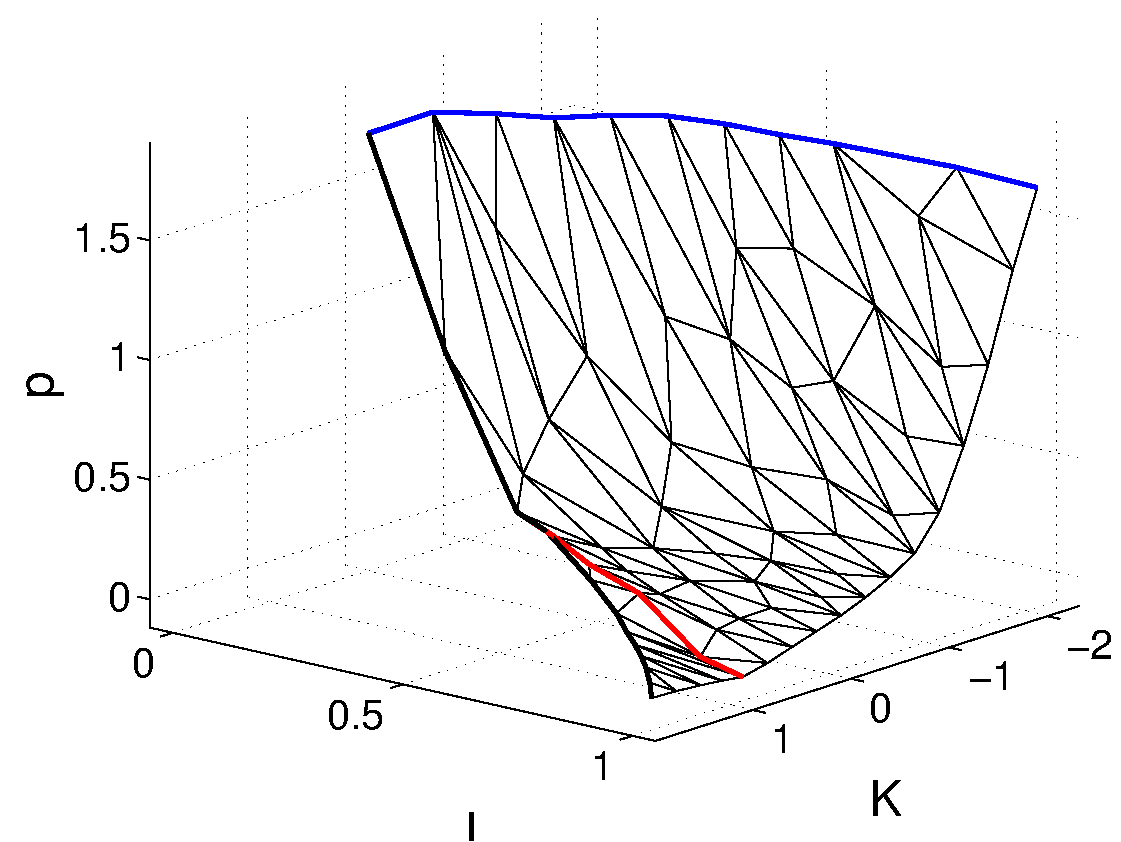
\includegraphics[width=\textwidth*7/8]{figures/db3_surf}
\caption{Probability density solution. Parameters are as the same as those for figure~\ref{f:drift diffusion figures}}
\label{f:FEM solution}
\end{center}
\end{figure}

With regards to physical significance of the solution, the main point to note is that the probability density function (PDF) is highest along the edge $K_{2I}$. This feature of the solution remains present when the aspect ratio of the cylindrical basin is varied from $d/a = 1$, as in Figure \ref{f:FEM solution} down to 0.3 (solution not illustrated.) In the X-Y phase plane, the edge $K_{2I}$ is situated outside the homoclinic orbit and our results suggests the wave motions most likely to be observed would be those corresponding to circular motion where for a given value of $I$, $K$ is near its maximum.

Similarly to our analysis, in \citet{miles84:_reson}, a system of two surface-gravity wave modes in a cylindrical basin subjected to horizontal excitation is studied. Unlike our problem, the two wave modes are set to be in exact resonance with one another, and a detuning parameter is introduced to represent the frequency difference between the natural wave frequency and the forcing frequency. A significant conclusion reached in that study is that for cylindrical basins with an aspect ratio between 0.3 and 0.5, limit cycles and chaotic motion are not possible, making the wave dynamics observed in that interval of aspect ratios qualitatively different from the dynamics seen outside that interval. In our case, with stochastic excitation, the probability densities obtained inside and outside the interval do not exhibit any qualitative differences; in both cases, the probability density is highest near the edge $K_{2I}$.

\section{Autoparametric Oscillator Solutions}

In this section, solutions for the autoparametric oscillator system are produced. The first set of solutions is shown in Figures \ref{f:fpe_sigma_1_area_100}, \ref{f:fpe_sigma_1_area_50} and \ref{f:fpe_sigma_1_area_10}. Physical parameters are kept the same for all of the solutions shown with the difference between the Figures being that different maximum areas for the elements are specified. The intent of these Figures is to demonstrate that across the gluing edge, where the finite element method must be formulated carefully, the solution does not exhibit any singularities. As the Figures show, the solutions appear to be continuous across the gluing edge, as expected based on analytic calculations.

\begin{figure}
\begin{center}
\psfrag{H}{$y_1$}
\psfrag{I}{$y_2$}
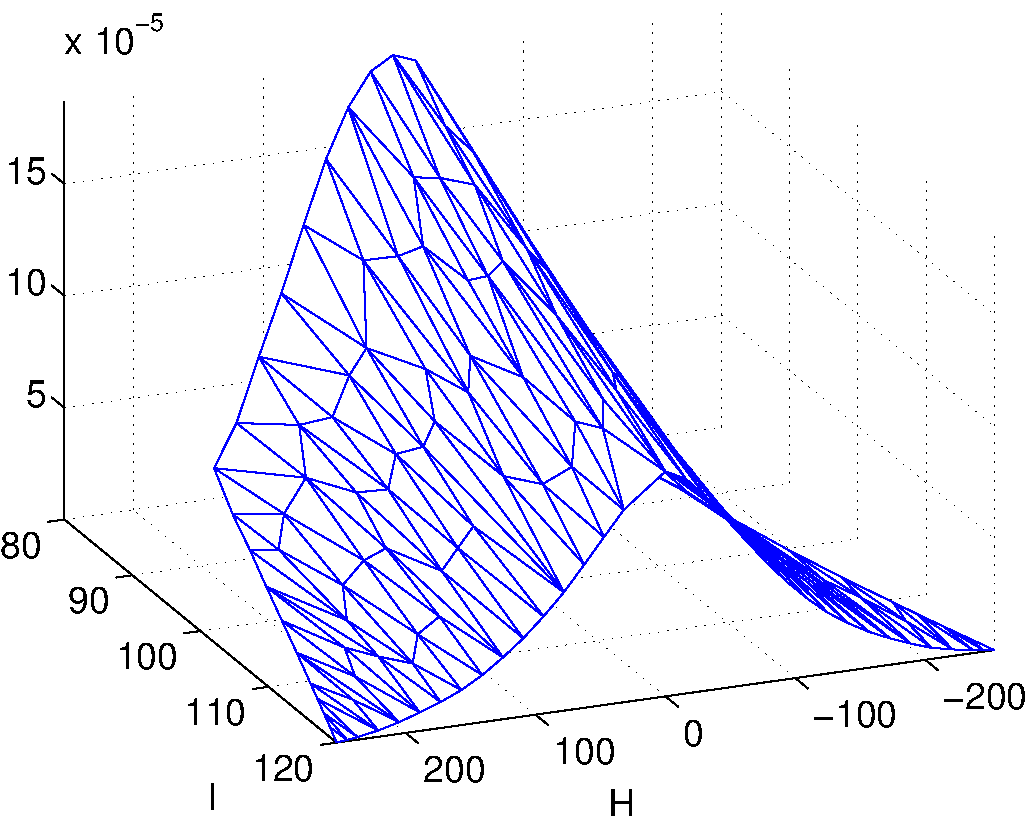
\includegraphics[width=\textwidth]{figures/fpe_solution_sigma_1_area_100}
\caption{Steady-state solution to the FPE obtained by the finite-element method when the maximum element area is 100.}
\label{f:fpe_sigma_1_area_100}
\end{center}
\end{figure}

\begin{figure}
\begin{center}
\psfrag{H}{$y_1$}
\psfrag{I}{$y_2$}
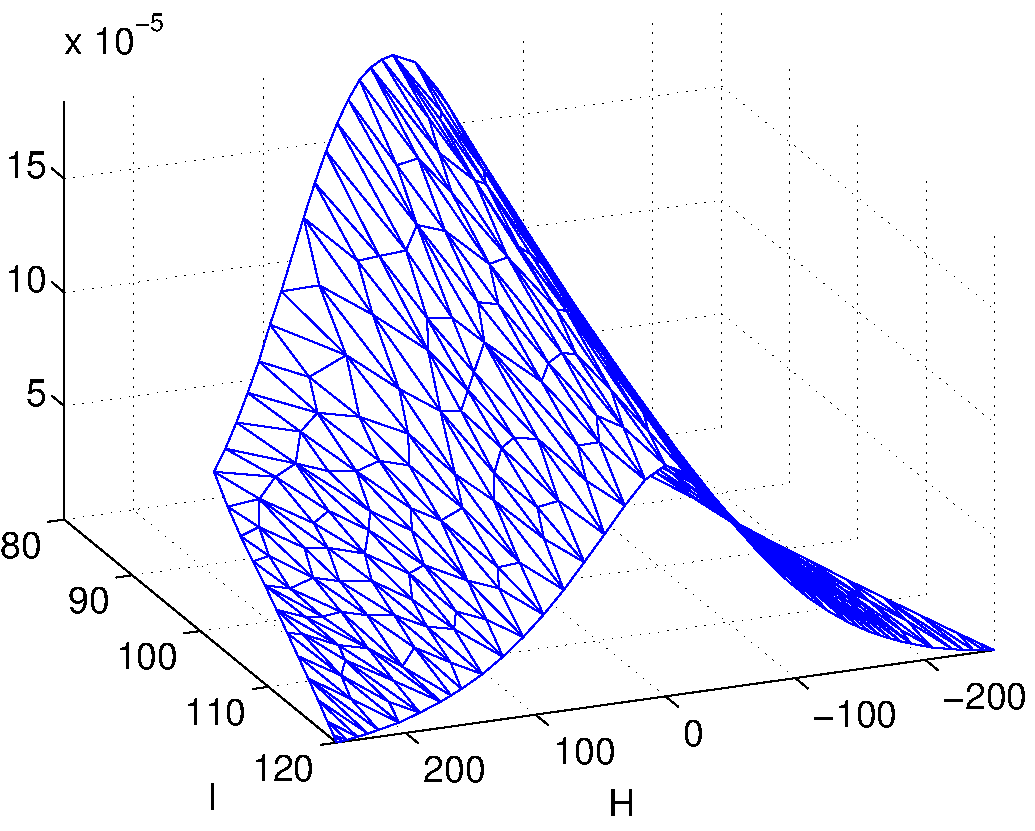
\includegraphics[width=\textwidth]{figures/fpe_solution_sigma_1_area_50}
\caption{Same solution as Figure \ref{f:fpe_sigma_1_area_100}, but with the maximum element area set to 50.}
\label{f:fpe_sigma_1_area_50}
\end{center}
\end{figure}

\begin{figure}
\begin{center}
\psfrag{H}{$y_1$}
\psfrag{I}{$y_2$}
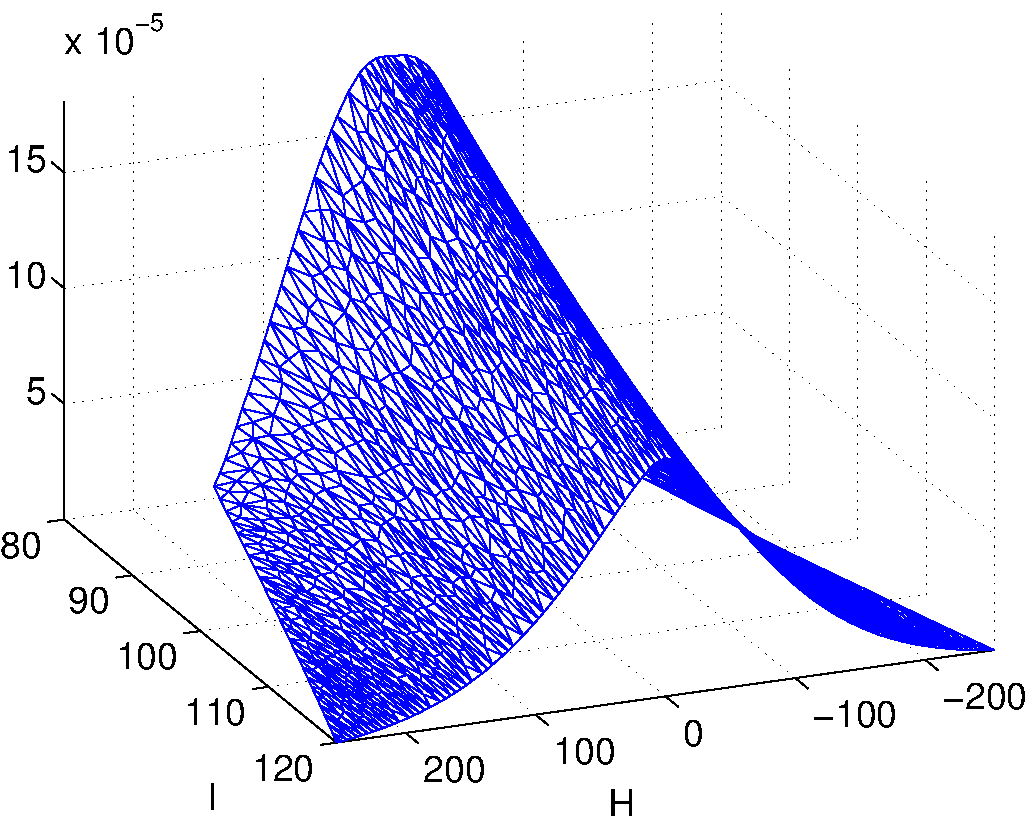
\includegraphics[width=\textwidth]{figures/fpe_solution_sigma_1_area_10}
\caption{Same solution as Figure \ref{f:fpe_sigma_1_area_100}, but with the maximum element area set to 10.}
\label{f:fpe_sigma_1_area_10}
\end{center}
\end{figure}

The next set of results is in shown in Figure \ref{f:fpe_sigma_1_i_lim}. These Figures probe the effect of varying the value of $I_\text{min}$. Recalling that the domain of the FPE has a cusp at the origin, the behavior of the solution near the origin is of interest. In Figure \ref{f:fpe_sigma_1_i_lim}, the FEM solution is plotted along the $I$-axis. Curves in that figure suggest that as the cusp is approached, the solution goes to zero.

\begin{figure}
\begin{center}
\psfrag{I}{$y_2$}
\psfrag{p}{$p$}
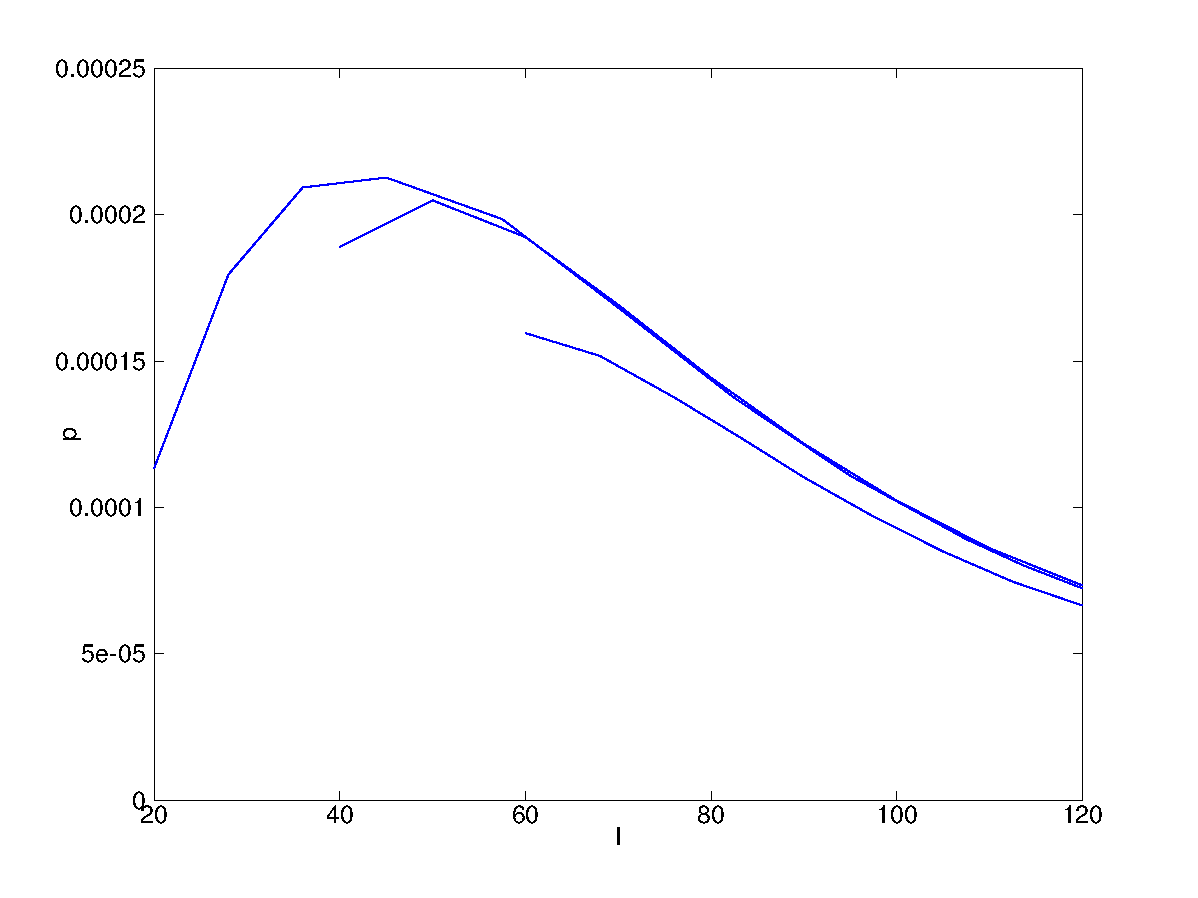
\includegraphics[width=\textwidth,clip=true,viewport=10 10 570 420]{figures/autoparam/i_lim}
\caption{Steady-state solution to the FPE along $y_1$ = 0 for different values of $y_{2,\text{min}}=20,40,60$. It is conjectured that the lines do not overlap exactly due to discretization errors.}
\label{f:fpe_sigma_1_i_lim}
\end{center}
\end{figure}

The final set of solutions is shown in Figures \ref{f:fpe_sigma_.5} and \ref{f:fpe_sigma_1.5}. These figures use the same mesh as Figure \ref{f:fpe_sigma_1_area_50}, but now a physically significant parameter, the amplitude of stochastic forcing, is varied. Although there seems to be a bug in the FEM solver that causes irregularities in the solution near the gluing edge, the overall trend in the solutions seems clear. As forcing amplitude is increased, the peak of the probability distribution moves to larger values of $I$ while remaining symmetric about the $I$ axis. The latter fact is worth contemplating. Recalling the structure of the Hamiltonian, (see Figure \ref{f:autoparam Hamiltonian}) the outer edge of the domain in the left hand plane corresponds to a sink and the outer edge of the domain in the right hand plane is a valley. As such it seems reasonable to think that as forcing amplitude increases, the peak of the PDF will shift from the left hand plane to the right hand plane, but this is not observed in the Figures. In fact, simply by looking at the form of $\mathfrak b_1$ (see Equations \eqref{e:b1 valley} and \eqref{e:b1 hill} and Figure \ref{F:b1_circ}), one notices that along the $K$ axis, the drift coefficient tends to center the probability density on the $I$ axis. It is curious that $\mathfrak b_1$ does not contain any stochastic effects; whether this is a generic feature for systems in 1:2 resonance remains to be determined.

\begin{figure}
\begin{center}
\psfrag{H}{$y_1$}
\psfrag{I}{$y_2$}
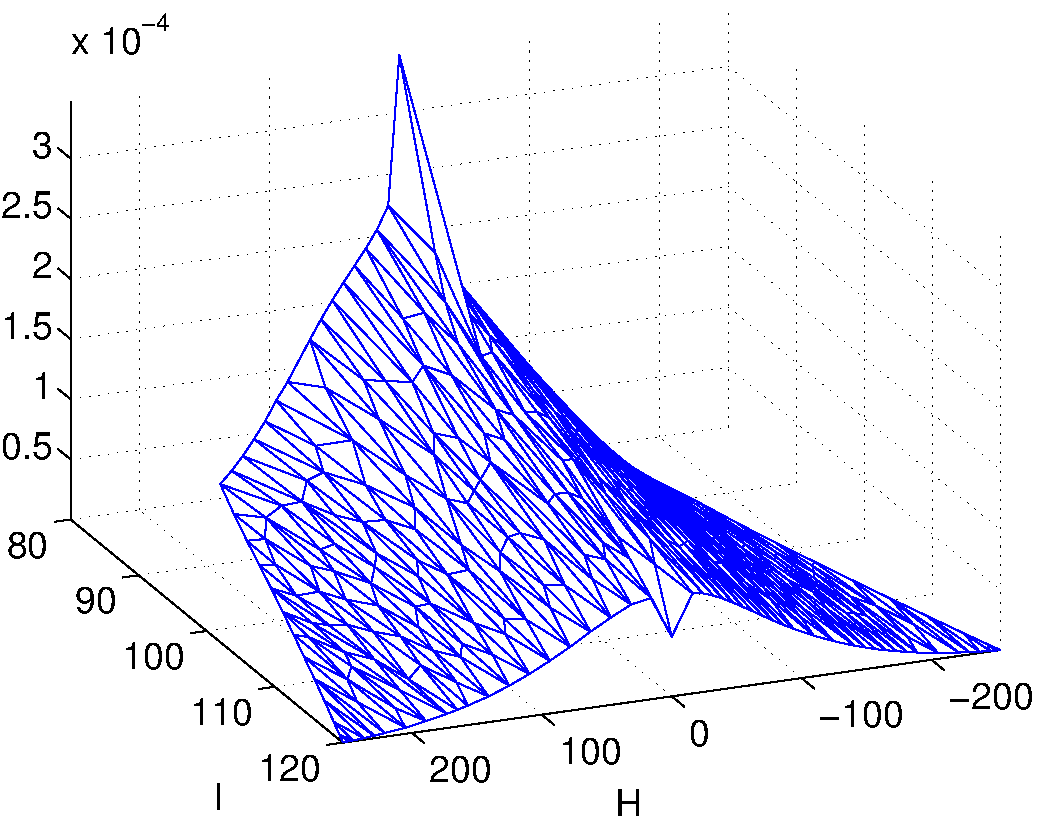
\includegraphics[width=\textwidth]{figures/fpe_solution_sigma_p5}
\caption{Steady-state solution to the FPE obtained by the finite-element method for $\sigma = 0.5$.}
\label{f:fpe_sigma_.5}
\end{center}
\end{figure}

\begin{figure}
\begin{center}
\psfrag{H}{$y_1$}
\psfrag{I}{$y_2$}
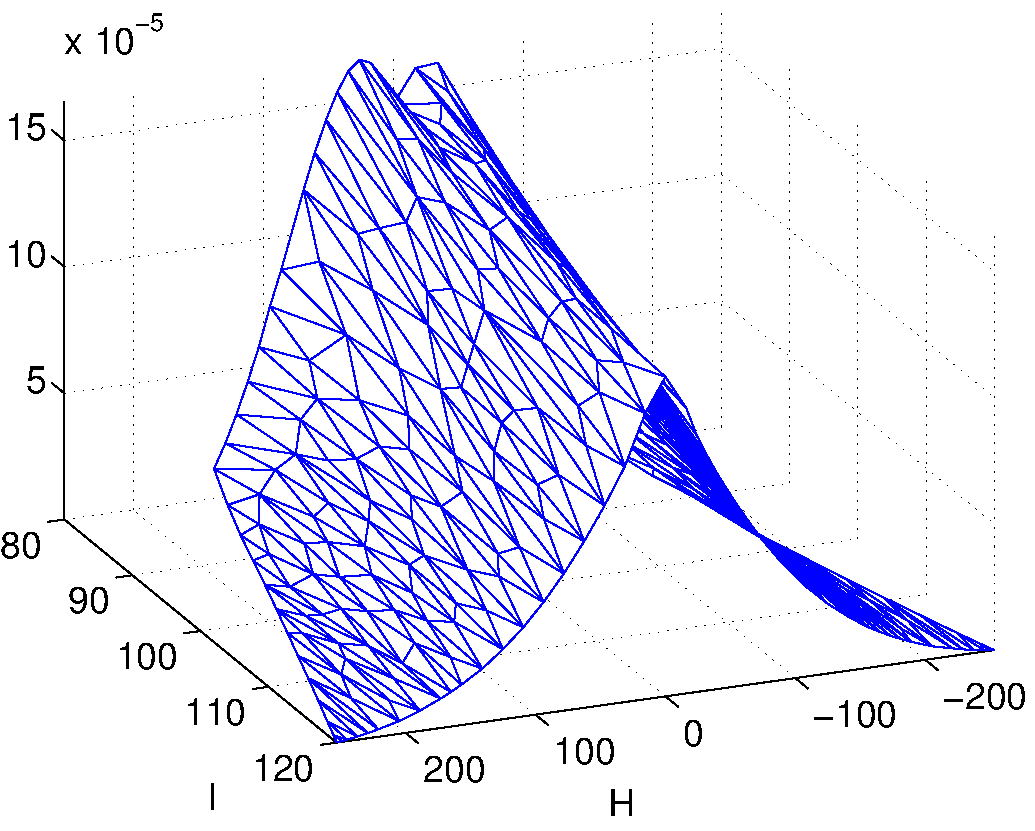
\includegraphics[width=\textwidth]{figures/fpe_solution_sigma_1p5}
\caption{Steady-state solution to the FPE obtained by the finite-element method for $\sigma = 1.5$.}
\label{f:fpe_sigma_1.5}
\end{center}
\end{figure}

\section{FEM Validation With Sample Path Method}

In this section, the solutions to the FPE obtained with the FEM are reproduced using an alternate approach. Instead of solving the FPE, the underlying stochastic differential equations are solved numerically. The validation method presented in this section can be used with the autoparametric and the wave systems, but results have been computed only for the autoparametric oscillator. The method presented was inspired by the heterogeneous multiscale method, as applied to stochastic differential equations \citep{e05:_analy}.

To begin, recall that unperturbed dynamics are governed by a Hamiltonian
\[
\dot z = \bar \nabla K, \quad z_0 \in \reals^4.
\]
After a canonical transformation, the dynamics of $z$ can be separated so that the fast dynamics are restricted to being in a 2-D plane. For the autoparametric oscillator, recalling Equation \eqref{E:vector-int}, the fast dynamics were given by
\begin{align*}
\dot u_1 &= - u_1 u_2, & \dot u_2 &= \frac12 (3 u_1^2 + u_2^2 - I).
\end{align*}
For the surface gravity wave model, similar 2-D fast dynamics are described by Equation \eqref{e:sgwaves fast planar}. These dynamics are obtained after time averaging and they are perturbed by higher order noise and damping effects. $X_t = (u_1,u_2)$ will be used as the fast variables and $Y_t = (K,I)$ will be the slow variables. Note that because $u_1, u_2$ and $K$ are constrained by Equation \eqref{E:AvgH}, it should be possible to have only one of the variables from the $(u_1,u_2)$ pair as the fast variable, but computationally it seems easier to use Equation \eqref{E:vector-int} than Equation \eqref{E:AvgH}. The general form of the fast equations is
\[
d X_t = \epsilon^{-2} f(X_t,Y_t) dt
\]
After time-averaging, the slow dynamics are given by
\begin{equation}
d \Tave[Y_t] = \epsilon^{-1} \Tave[F^2](X_t,Y_t) dt + \epsilon^{-2} \Tave[G](X_t,Y_t) dt.
\end{equation}
It is important to understand why the dynamics of the slow variables are time averaged. Prior to time averaging, the equation for $Y_t$ contains a term of order $\epsilon^{-2}$, therefore the dynamical timescales of the fast and slow equations are not separated. It should be possible to perform $\Tave$-averaging numerically, but for simplicity, here time averaged quantities are considered straightaway.
The averaged equation is
\begin{equation}
\label{e:averaged}
d\Aave[\Tave[Y_t]] = \Aave[\Tave[m]](Y_t) dt + \Aave[\Tave[\sigma]](Y_t) dt
\end{equation}
with $m$ defined in Equation \eqref{E:drift2} and $\sigma$ will be derived from \eqref{E:diffusion2}. Conceptually, $\Aave$-averaging represents averages over Hamiltonian orbits.

Having described the two timescale nature the equations to be solved, now the numerical procedure is setup. Since the fast dynamics are deterministic, the equivalent of what is called the \emph{microsolver} in the HMM can be implemented using widely available numerical ODE solvers. The microsolver serves to generate paths over which to calculate the averaged coefficients, symbolically
\[
\Aave[f](y) = \frac{1}{T(y)} \int_0^{T(y)} f(X_t, y) dt.
\]
For simplicity analytic results of Chapter \ref{c:autoparametric} are used for $T(y)$, but in principle this quantity could be discovered with the microsolver. Note that in \citet{e05:_analy} the case where the fast equations are stochastic is treated; this can make the choice of an optimal time-span for the microsolver more difficult. Referring to terminology used in the HMM context, an \emph{estimator} is used to approximate the averaging operator. The estimator resembles numerical integration formulas:
\[
\frac{1}{T(y)} \sum_{i=1}^N f(u(t_i),y) \Delta t_i.
\]
Thus estimated values for $\Aave[\Tave[m]]$ and $\Aave[\Tave[\sigma \sigma^T]]$ are obtained. Let us denote these estimates by $\tilde{\mathfrak b}$ and $\tilde{\mathfrak a}$ respectively. Because the fast equations are deterministic, the computations performed by the microsolver and estimator for the problems considered in this thesis are rather simple. Nonetheless, they make it possible to validate the results obtained analytically for the autoparametric oscillator and the results obtained with numerical quadrature for the surface gravity waves system. Comparisons between the analytically obtained drift and diffusion coefficients and their estimated values show good agreement (typically differences smaller than $10^{-8}$.)

Whereas averaging provides the diffusion matrix $\mathfrak{a} = \Aave[\Tave[\sigma \sigma^T]]$, to produce sample paths, $\sigma$ is needed. Cholesky decomposition is used to make this connection. Symbolically, let's use the notation
\[
\tilde{\mathfrak a} = \tilde \sigma \tilde \sigma^T.
\]
The key point is that the variance of $\tilde{\mathfrak a}$ is reproduced when $\tilde \sigma^T$ multiplies a Wiener process \citep{law82:_simul}.

In the HMM, the slow equations are approximated numerically with the \emph{macrosolver}. For numerical solutions to System \eqref{e:averaged}, a stochastic ODE solver is used. The simplest of these is the Euler-Maruyama first order scheme \citep{kloeden92:_numer_solut_stoch_differ_equat}:
\[
Y_{n+1} = Y_n + \tilde{\mathfrak b}_n \Delta t + \tilde \sigma_n \Xi_{n+1} \sqrt{\Delta t}
\]
where $\Xi_n$ are normally distributed random numbers with mean zero and variance one. This completes the description of the numerical method used to generate stochastic samples in a multiscale context. An analysis of the convergence properties and efficiency of the scheme presented here has not been performed.

In order to validate the solutions obtained by the FEM multiple sample paths must be produced. This can be done systematically with the following procedure. First, initial conditions must be generated so as to reproduce a uniform distribution across the entire $K-I$ domain. First a FEM triangulation is produced and the area of each element is calculated. The initial conditions of the samples are set at the center of each element, and the number of samples in each element is proportional to each element's area. Such a placement scheme is automated by dividing the unit interval into segments with length proportional to each element's area. A uniform random number generator is then used to draw numbers in the unit interval and the number of samples placed at the center of each element is determined by the uniform random number generator. Thus larger elements end up with more samples and smaller elements with fewer.

At each time-step of the macrosolver, the microsolver is initialized with conditions consistent with the state of the macrosolver. The microsolver is then simulated for the time-span of one period so as to compute the values of $\tilde{\mathfrak b}$ and $\tilde{\mathfrak a}$. In order to impose reflective boundary conditions, at each step of the macrosolver a check is made to determine if the sample has gone outside the domain. If it has, the sample is returned to its last location inside the domain, but the time-step is still increased by one. This approach ensure that the reflective boundary condition does not lead to infinite simulation times.

% FIXME Provide pseudo-code of the function macrosolver_ic here.

All the samples are simulated for an equal number of time-steps of the macrosolver. The number of samples in each element is then counted and the value of each node is set by taking the average of the number of samples of all the elements that contain that node.

% FIXME The average should, perhaps, be weighed by the element areas.

Results produced with this numerical approach are shown in Figures \ref{f:hmm sigma=.5} to \ref{f:hmm sigma=1.5}. These results bear a qualitative resemblance to the FEM results. Namely, as the noise intensity is increased, the probability distributions move away from the origin, but remain centered around the $K=0$ axis. The solutions shown in the Figures are not particularly smooth. Presumably smoother solutions could be produced, but producing the Figures shown takes several hours. Optimizing numerical parameters such as the time-step of the Euler-Maruyama solver and the time-span of the macrosolver may be necessary to avoid excessively long simulations.

\begin{figure}
\begin{center}
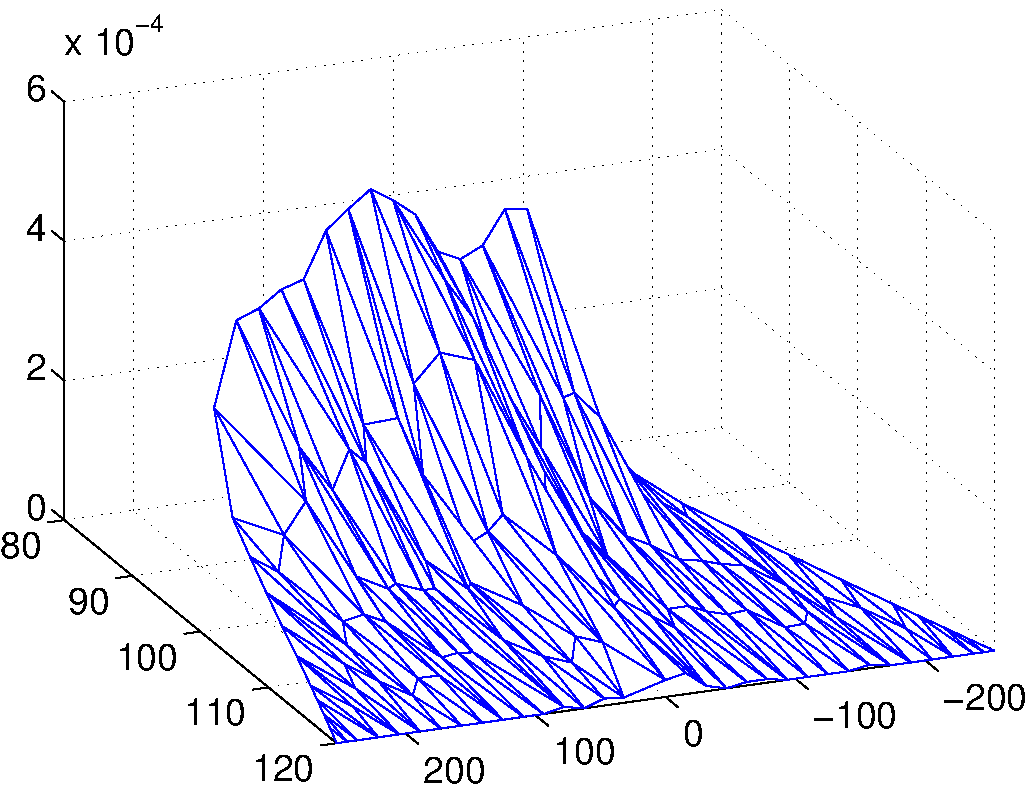
\includegraphics[width=\textwidth]{figures/hmm_pdf_sigma_p5}
\end{center}
\caption{HMM solution for $\sigma = 0.5$. 1000 samples are used to produce this PDF.}
\label{f:hmm sigma=.5}
\end{figure}

\begin{figure}
\begin{center}
\label{f:hmm sigma=1}
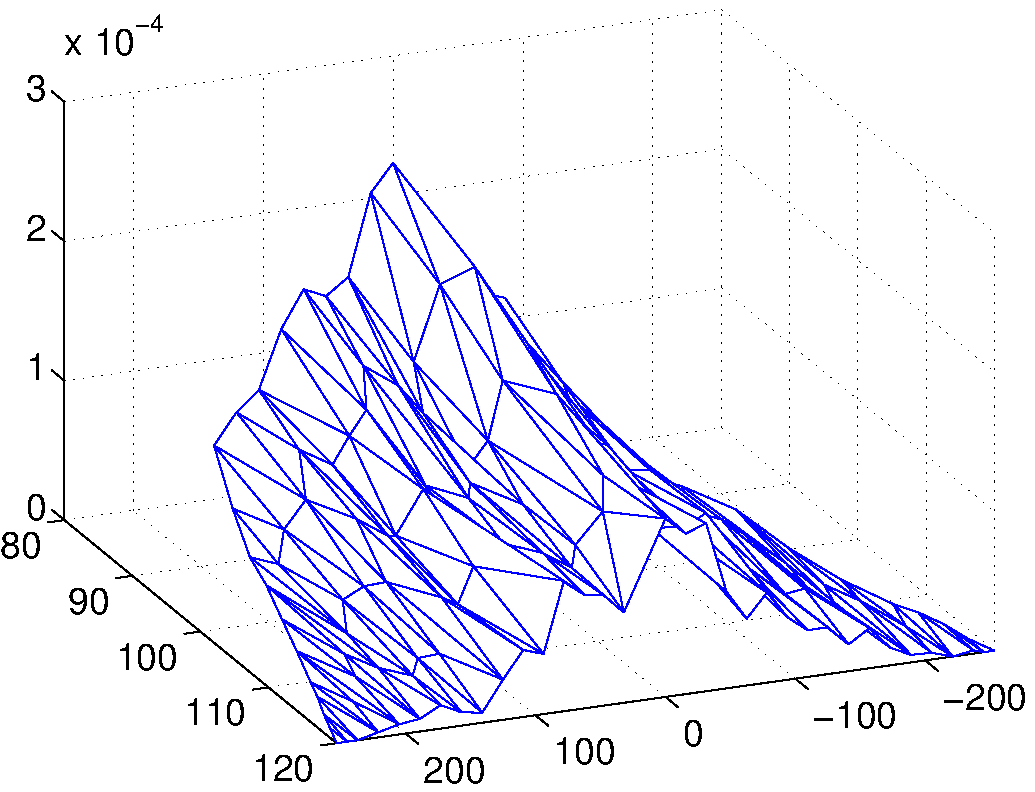
\includegraphics[width=\textwidth]{figures/hmm_pdf_sigma_1}
\end{center}
\caption{HMM solution for $\sigma = 1$. 2000 samples are used to produce this PDF.}
\end{figure}

\begin{figure}
\begin{center}
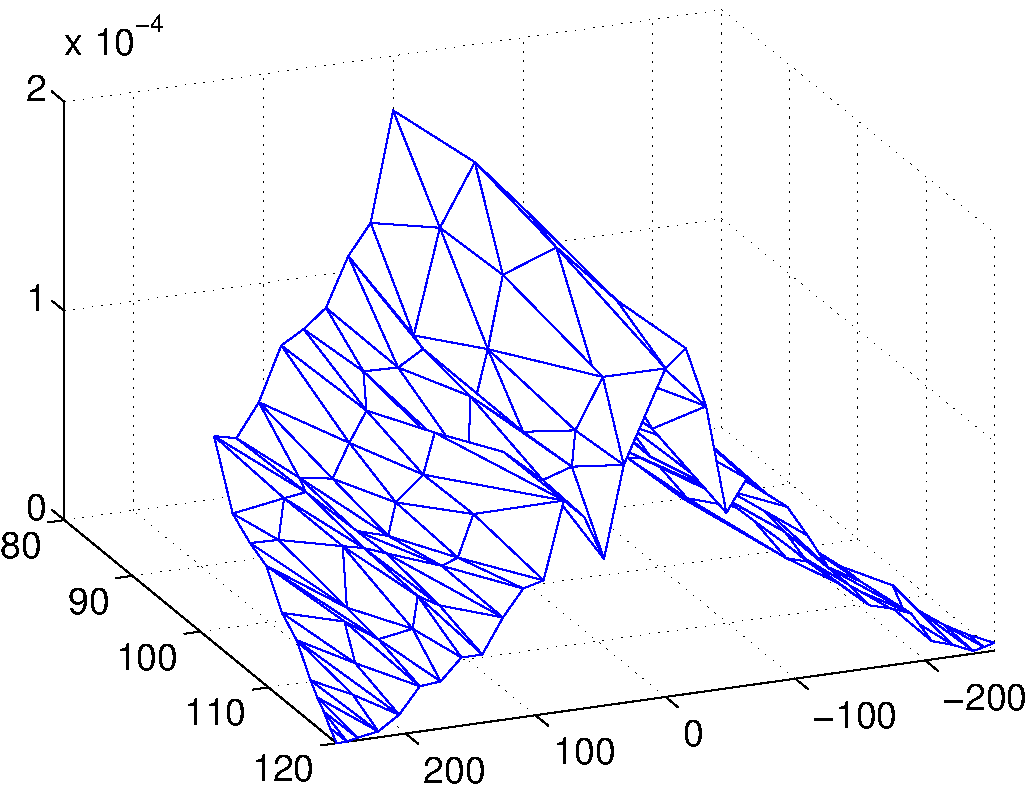
\includegraphics[width=\textwidth]{figures/hmm_pdf_sigma_1p5}
\end{center}
\caption{HMM solution for $\sigma = 1.5$. 4000 samples are used to produce this PDF.}
\label{f:hmm sigma=1.5}
\end{figure}

It is worth mentioning that producing the solutions shown in Figures \ref{f:hmm sigma=.5} to \ref{f:hmm sigma=1.5} takes several hours whereas the solutions produced with the FEM takes no more than a few minutes. Establishing exact figures on the computational advantage of FEM methods over SDE methods would require additional work; numerical parameters should be chosen optimally. Nonetheless, the large difference in computation times between the two methods suggests that averaging methods can lead to significantly faster computational methods. It seems plausible that in some circumstances, problems that have been deemed too complicated could be solved if stochastic averaging methods were used.

%%% Local Variables: 
%%% mode: latex
%%% TeX-master: "main"
%%% End:


% The Fokker--Planck equation
% Finite Element Formulation
% Solutions for the Surface Gravity Waves Problem
% Solutions for the Autoparametric Oscillator
% Validation With a Sample Path Method

\chapter{Conclusions}
\label{c:conclusions}
Summarizing the results of this thesis, the theory of stochastic averaging has been applied to study the behavior of mechanical systems with bifurcations in their fast deterministic dynamics. After setting the systems near low-order resonance, the reduced space of the averaged systems was determined. Stochastic averaging theory was then applied to calculate drift and diffusion coefficients of the reduced Markov process. The steady response of the systems has been characterized by finding solutions of the Fokker--Planck equation. From a physical point of view, the solutions obtained exhibit peculiarities that are not anticipated from deterministic analysis. A comprehensive interpretation of these peculiarities remains an open area of research.

In closing this thesis, possible extensions are covered.

% Physical issues with wave model
A number of things could be done to improve physical insight into the surface waves problem. Two of the easiest extensions would be to (i) carry out calculations for vertical forcing and (ii) carry out calculations for 1:2 resonance. Given that analytical formulas have been found for the autoparametric problem in 1:2 resonance, it would be interesting to see if the same could be achieved with the surface wave equations.

The Miles wave model presented in Section \ref{s:governing equations} is highly idealized. To make the model more realistic, surface tension could be added. The potential energy with surface tension terms is given in~\citet{miles90:_param_forced_surfac_waves}:
\[
V = \rho S(-Q_n q_n) + \frac12(g + \ddot{z}) q_n q_n + \frac12 \hat{T} (\delta_{mn} k^2_n - \frac{1}{4} b_{jlmn} q_j q_l + \Order(q^3)) q_m q_n
\]
$\rho \hat{T}$ is the surface tension. It should be straightforward to replace Equation \eqref{e:potential energy}. Since surface tension, like gravity, acts on terms quadratic in $q$, and because the averaged drift and diffusion coefficients do not vanish, the inclusion of surface tension effects should lead to quantitative but not qualitative changes in the averaging results.

In the surface wave model, linear damping has been used. It would be good if the fluid viscosity could be related to the damping coefficients. This may allow the removal of damping terms as free parameters. The work presented in \citet{vega01:_nearl_invis_farad_waves} may provide a good starting point since it uses a model similar to the Miles wave model.

% Resonant wave triads & turbulence

The averaging results presented in this thesis have used a Hamiltonian and an angular momentum as the slow variables. For the models analyzed, there is little doubt that these are the optimal slow variables. For other applications finding slow variables can be non-trivial. Therefore, developing automated methods to select slow variables, such as the method based on anisotropic diffusion maps \citep{singer09:_detec} seems worthwhile.

With regards to applications of stochastic averaging theory, this thesis has presented steady probability densities obtained from the Fokker--Planck equation as the ultimate application. Another application frequently sought for engineering applications is the calculation of exit times from a prescribed domain. Once the averaged drift and diffusion coefficients are known, calculating exit times should not require much more work. For the problems presented here, one could calculate the exit time associated with different values of $I_\text{max}$.

Steady solutions of the Fokker--Planck equation have been obtained directly. For certain applications, it may be desirable to know the transient behavior of the FPE. For example, in filtering problems one seeks to merge theoretically predicted dynamics with experimentally obtained data. This requires time-dependent solutions.

Another numerical aspect that could be explored is the nature of the Fokker--Planck equation as a convection-diffusion equation. The numerical methods required to solve convection-diffusion equations can change dramatically depending on the magnitude of the convective terms relative to the diffusive terms. While the steady solutions produced seem acceptable, it may be that for time-dependent solutions a detailed understand of numerical methods for convection-diffusion PDEs will be necessary, particularly since the drift and diffusion coefficients can vary greatly near gluing vertices.

The FEM used to solve the Fokker--Planck equation has not been analyzed for numerical convergence properties. It appears that this is an areas that it still open for research. \citet{kumar09:_fokker_planc} provide some results in this direction, however their work uses spectral decompositions and as such, may be difficult to apply to domains like the ones encountered in this thesis, with non-trivial shapes.

In finding reduced domains, it has been observed that for both the surface waves and autoparametric oscillator models, a cusp exists at the gluing boundary that joins two fixed points. To obtain solutions, this issue has been ``swept under the rug'' by removing the portion of the domain that contains the cusp and by imposing reflective boundary conditions instead. While it has been demonstrated numerically that such an approach gives reasonable solutions, it would be good to analyze this problem analytically. For this, the first step might be to study the one-dimensional diffusion process along the gluing edge. For one dimensional diffusions one might start by calculating scale and speed measures\cite[\S 15.6]{karlin81:_secon_cours_stoch_proces}.

The numerical scheme devised in the second half of Chapter \ref{c:pdf} was inspired by the heterogeneous multiscale methods\citep{e05:_analy}. To keep the analysis simple, the fastest of the three timescales in our mechanical systems was not incorporated. Developing a three timescale HMM should be possible, and this would form a more complete counterpart, and validation method, to the stochastic averaging method.

% Scaling parameter \epsilon does not have a physical significance

% Second-order averaging for surface waves

% Explain why reflective boundary conditions are imposed

%%% Local Variables: 
%%% mode: latex
%%% TeX-master: "main"
%%% End: 


\appendix
\chapter{Surface Gravity Waves}
\section{Non-linear Hamiltonian}
\label{a:non-linear Hamiltonian}

The equation below give the detailed form of terms appearing in non-linear Hamiltonian coefficient appearing in Equation~\ref{e:hamiltonian coefficient expansion}. These expressions are copied from \citep{miles76:_nonlin}.
\begin{equation}
h_{lmn} = D_{lmn} - C_{lmn} k_m k_n
\end{equation}
\begin{equation}
h_{jlmn} = D_{jlmn} (k_m + k_n) - 2 C_{jmi} D_{lni} k_m - 2 C_{lni} D_{jmi} k_n + 2 C_{jmi} C_{lni} k_i k_m k_n
\end{equation}
\begin{equation}
C_{lmn} = S^{-1} \iint \psi_l \psi_m \psi_n dS
\end{equation}
\begin{equation}
C_{jlmn} = S^{-1} \iint \psi_j \psi_l \psi_m \psi_n dS
\end{equation}
\begin{equation}
D_{lmn} = S^{-1} \iint \psi_l \nabla \psi_m \cdot \nabla \psi_n dS
\end{equation}
\begin{equation}
D_{jlmn} = S^{-1} \iint \psi_j \psi_l \nabla \psi_m \cdot \nabla \psi_n dS
\end{equation}

Formulas for the eigenfunctions, $\psi_k$, are determined by the geometry of the wave basin. For a cylindrical tank, complete specifications are given in \citet{miles84:_inter}.

% FIXME Add formulas for \psi_1 and \psi_2

\section{Drift and Diffusion Coefficient Integrands}
\label{a:drift and diffusion coefficient integrands}

The results given below are for the case of horizontal forcing.

\begin{multline}
\Tave(F^2_H) = \frac{k^2 \omega^2}{48 g}\Big\{\alpha_1 \big[K_1 (\{X^2 + Y^2\} X^2 + I\{X^2 + 3Y^2\})\\
+ 16 K_{-1} (2I - X^2 - Y^2) X^2\big]\\
+ \alpha_2 \big[2I - X^2 - Y^2\big] \big[3 K_1 I - (K_1 - 16 K_{-1}) X^2 \big]\Big\}\\
+ \frac12 (\sigma_1 \alpha_1 - \sigma_2 \alpha_2) (X^2 + Y^2) + \sigma_2 \alpha_2 I
\end{multline}
\begin{multline}
\Tave(\mathfrak{g}_H) = \frac{\sqrt{2 \pi}}{24} \frac{x_{11}^2 \ \omega \mathcal{F}_c(\omega)}{g^2 S^2} \big\{k^2 \omega^2 [(K_1 - 4 K_{-1})(X^2 + Y^2) + (K_1 + 8 K_{-1}) I ]\\
+ 12 g \sigma_1 \big\}
\end{multline}
\begin{equation}
\Tave(F^2_I) = \frac12 \big[(\alpha_1 - \alpha_2) (X^2+Y^2) + 2 \alpha_2 I \big]
\end{equation}
\begin{equation}
\Tave(\mathfrak{g}_I) = \frac{\sqrt{2 \pi} x^2_{11} \omega \mathcal{F}_c(\omega)}{2 g S^2}
\end{equation}
\begin{multline}
\Tave(\sigma \sigma^T)_{HH} = \frac{\sqrt{2 \pi} x^2_{11} \omega \mathcal{F}_c(\omega)}{1152 g^3 S^2}\big[k^4 \omega^4 \{256
K_{-1}^2 X^2 (X^2 + Y^2 - 2I)\\
- 32 K_1 K_{-1} X^2 [(X^2+Y^2)^2 - I(X^2+Y^2) - 2I^2]\\+ K_1^2 [2IX^2(X^2 + Y^2) + X^2(X^2 + Y^2)^2 + I^2(X^2 + 9Y^2)] \}\\
+ 48 g k^2 \omega^2 \sigma_1 \big\{K_1(IX^2 + X^4 + 3 I Y^2 + X^2 Y^2) + 16 K_{-1} X^2 (2I - X^2 - Y^2) \big\}\\
+ 576 g^2 \sigma_1^2(X^2 + Y^2) \big]
\end{multline}
\begin{multline}
\Tave(\sigma \sigma^T)_{HI} = \frac{\sqrt{2\pi} x_{11}^2 \omega \mathcal{F}_c(\omega)}{48 g^2 S^2} \big[k^2 \omega^2 \{K_1 (I X^2 + X^4 + 3IY^2 + X^2Y^2)\\
+ 16 K_{-1} X^2 (2I - X^2 - Y^2)\} + 24 g \sigma_1 (X^2 + Y^2) \big]
\end{multline}
\begin{equation}
\Tave(\sigma \sigma^T)_{II} = \frac{\sqrt{2 \pi} x^2_{11}
\omega \mathcal{F}_c(\omega )}{2 g S^2} (X^2 + Y^2)
\end{equation}


\chapter{Autoparametric System}
\section{Nonlinear vector fields}
\label{A:autoparam nonlin vec fields}

In this appendix, we derive exact formulae for $b^1$ and $b^2$ in~\eqref{E:standard1}. Although quadratic nonlinearities in coupled oscillators affect the normal froms or the averaged equations at higher order, the presence of $1:2$ resonance make their contribution at ${\Order}(\epsilon)$ paramount. For the problem under consideration, we have:
\begin{align*}
b^1_1(x,t) &= \frac{1}{4} (x_2^2 - x_4^2) [\sin(2q + 1)t + \sin(2q - 1)t]\\
&\quad - \frac12 x_2 x_4 [\cos(2q + 1)t + \cos(2q - 1)t]\\
% b^1_2(x,t) &= \frac12 \left(x_1x_4 - x_2x_3\right)\cos(2q - 1)t + \frac12 \left(x_1x_2 - x_4x_3\right) \sin(2q + 1)t\\
% &\quad - \frac12 \left(x_1x_2 + x_3x_4\right) \sin(2q - 1)t - \frac12 \left(x_1x_4 + x_2x_3\right) \cos(2q + 1)t\\
b^1_2(x,t) &= \frac12 (x_1 x_2 - x_3 x_4) [\sin(2q + 1)t - \sin(2q - 1)t]\\
&\quad + \frac12 x_1 x_4 [\cos (2q - 1)t - \cos(2q + 1)t]\\
&\quad - \frac12 x_2 x_3 [\cos(2q - 1)t + \cos(2q + 1)t]\\
b^1_3(x,t) &= \frac14 (x_2^2 - x_4^2) [\cos(2q - 1)t - \cos(2q + 1)t]\\
&\quad - \frac12 x_2 x_4 [\sin(2q + 1)t - \sin(2q - 1)t]\\
% b^1_4(x, t) &=\frac12 \left(x_1 x_2 + x_3 x_4\right) \cos(2q - 1) t - \frac12 \left(x_1 x_4 + x_2 x_3\right) \sin(2q + 1)\\
% &\quad + \frac12 \left(x_1 x_4 - x_2 x_3\right) \sin(2q - 1) t + \frac12 \left(x_4 x_3 - x_2 x_1\right) \cos(2q + 1) t
b^1_4(x,t) &= \frac12 x_1 x_2 [\cos(2q - 1)t - \cos(2q + 1)t]\\
&\quad - \frac12 x_1 x_4 [\sin(2q + 1)t - \sin(2q - 1)t]\\
&\quad - \frac12 x_2 x_3 [\sin(2q - 1)t + \sin(2q + 1)t]\\
&\quad + \frac12 x_3 x_4 [\cos(2q - 1)t + \cos(2q + 1)t]
\end{align*}
In these expressions, those terms that contain $\cos(2q - 1)t$ will remain constant while averaging with the condition of resonance, i.e., $q=1/2$.

At $\Order(\epsilon^2)$, we consider the cubic nonlinearities of the original equations of motion, the dissipative effects and the effect of detuning. It is worth pointing out that, while averaging there will be higher order terms from the quadratic nonlinearities,and they have to be considered at ${\Order}(\epsilon^2)$ to be consistent.
\begin{align*}
b^2_1(x,t) &= -\zeta_o x_1 + \frac{1}{4q} x_3 \left({x_2}^2+{x_4}^2\right) + \frac{1}{4q} {x_3 \left({x_2}^2+{x_4}^2\right)\cos(2t)}\\
&\quad + \frac{1}{8q} {\left(2\,x_2x_4x_1+{x_2}^2 x_3-{x_4}^2 x_3\right) \cos(1 + q)2\,t}\\
&\quad - \frac{1}{8q}\,{ \left(-{x_2}^2 x_3 + {x_4}^2 x_3 + 2\,x_2 x_4 x_1\right) \cos(q-1)2\,t}\\
&\quad + \frac{1}{4q}{x_3 \left(x_2 - x_4\right) \left(x_2 + x_4 \right) \cos(2\,qt)}\\
&\quad - \frac{1}{8q}\,{\left(-{x_4}^2x_1+{x_2}^2x_1 - 2\,x_2 x_4 x_3\right) \sin(1+q)2\,t}\\
&\quad + \frac{1}{8q}\, {\left({x_2}^2 x_1 + 2\, x_2 x_4 x_3 - {x_4}^2x_1\right)\sin(q-1)2\,t}\\
&\quad - \frac{1}{4q} {x_1\left({x_2}^2+{x_4}^2\right)\sin(2\,t)} + \frac{1}{2q} {x_2x_4x_3\sin(2\,qt)}\\
&\quad + \zeta_o x_1\cos(2t) + \zeta_ox_3 \sin(2\,t)
\end{align*}
\begin{align*} 
b^2_2(x,t) &= -\frac{1}{2q} \left({2 \zeta_p q x_2 - \mu x_4}\right)\\
&\quad+\frac{1}{16{Rq}}\,{x_4\left(4\,R \,({x_1}^2 + {x_3}^2) + (4\,Rq - q)({x_2}^2
+ {x_4}^2) \right)}\\
&\quad-\frac{1}{4q}{x_4\left(x_1-x_3\right)\left(x_1 + x_3\right)\cos(2t)}\\
&\quad+\frac{1}{8q}\,{\left(2\,x_2x_1 x_3+x_4{x_1}^2-x_4{x_3}^2\right)\cos(1+q)2t}\\
&\quad+\frac{1}{8q}\,{\left(-x_4{x_3}^2+x_4{x_1}^2 - 2\,x_2x_1x_3\right)\cos(q-1)2\,t}\\
&\quad-\frac{1}{12Rq}\,{ x_4 \left(3\,R{x_3}^2+3\,R{x_1}^2-q{x_4}^2\right)\cos(2\,qt)}\\
&\quad+\frac{1}{48{R}}\,{x_4\left(-{x_4}^2+3\,{x_2}^2\right)\left(1+12\,R\right)\cos(4\,qt)}\\
&\quad-\frac{1}{8q} {\left(-2\,x_4x_1x_3+x_2{x_1}^2-x_2{x_3}^2\right)\sin(1+q)2\,t}\\
&\quad-\frac{1}{8q}\,{\left(x_2{x_1}^2+2\,x_4x_1x_3-x_2{x_3}^2\right)\sin(q-1)2\,t}\\
&\quad-\frac{1}{48{R}}\,{x_2\left({x_2}^2-3\,{x_4}^2\right)\left(1+12\,R\right)\sin(4\,qt)}\\
&\quad-\frac{1}{2q}\,{x_4x_1x_3\sin(2\,t)}\\
&\quad+\frac{1}{24{Rq}} x_2 \left(-q{x_2}^2+6\,R{x_1}^2 + 6\,R{x_3}^2 - 3\,q{x_4}^2\right) \sin(2qt)\\
&\quad+\frac{1}{2q}\,{\left(2\,\zeta_pqx_2-\mu\,x_4 \right) \cos(2\,qt)}+\frac{1}{2q}\,{\left(\mu\,x_2+2\,\zeta_2qx_4\right)\sin(2\,qt)}
\end{align*}
\begin{align*}
b^2_3(x,t) &= -\zeta_o x_3 - \frac{1}{4q}{x_1\left({x_2}^2+{x_4}^2\right)}+ \frac{1}{4q}{x_1\left({x_2}^2 + {x_4}^2 \right) \cos(2t)}\\
&\quad + \frac{1}{8q}\,{\left(-{x_4}^2 x_1 + {x_2}^2 x_1 - 2\,x_2 x_4 x_3\right)\cos(1+q)2t}\\
&\quad +\frac{1}{8q}\,{\left
    ({x_2}^2x_1+2\,x_2x_4x_3-{x_4}^2x_1
   \right)\cos(q-1)2\,t}\\
&\quad - \frac{1}{4q}{x_1\left
    (x_2-x_4\right)\left(x_2+x_4\right)\cos
   (2\,qt)}\\
&\quad+\frac{1}{8q}\,{\left
    (2\,x_2x_4x_1+{x_2}^{2
    }x_3-{x_4}^2x_3\right)\sin(1+q)2\,t}\\
&\quad+\frac{1}{8q}\,{\left
    (-{x_2}^2x_3+{x_4}^2x_3+2\,x_2
    x_4x_1\right)\sin(q-1)2\,t}\\
&\quad+\frac{1}{4q}{x_3\left({
     x_2}^2+{x_4}^2\right
   )\sin(2\,t)}-\frac{1}{2q}\,{x_2
   x_4x_1\sin(2\,qt)}+\zeta_ox_1\sin(2\,t)\\
&\quad- \zeta_o x_3 \cos(2t)
\end{align*}
\begin{align*}
b^2_4(x,t) &= - \frac{1}{2q} \left(\,{\mu\,x_2 + 2\,\zeta_p q x_4}\right)\\
&\quad- \frac{1}{16{Rq}}\,{x_2 \left(4\,R \,({x_1}^2 + {x_3}^2) + (4\,Rq - q)({x_2}^2 + {x_4}^2) \right)}\\
&\quad + \frac{1}{4q}{x_2\left (x_1-x_3\right) \left(x_1+x_3\right)\cos(2t)}\\
&\quad + \frac{1}{8q}\,{ \left(-2\,x_4x_1x_3+x_2{x_1}^2-x_2{x_3}^2\right)\cos(1+q)2t}\\
&\quad +\frac{1}{8q}\,{\left(x_2{x_1}^2+2\,x_4x_1x_3-x_2{x_3}^2\right)\cos(q-1)2\,t}\\
&\quad -\frac{1}{12{Rq}}\,{x_2\left(3\,R{x_3}^2-q{x_2}^{2}+3\,R{x_1}^2\right)\cos(2\,qt)}\\
&\quad + \frac{1}{48{R}}\,{x_2 \left({x_2}^2 - 3{x_4}^2\right) \left(1+12\,R\right)\cos(4\,qt)}\\
&\quad + \frac{1}{8q} {\left(2\,x_2x_1x_3 + x_4{x_1}^2 - x_4{x_3}^2\right)\sin(1+q)2\,t}\\
&\quad + \frac{1}{8q} {\left(-x_4{x_3}^2+x_4{x_1}^2-2\,x_2x_1x_3\right)\sin(q-1)2\,t}+\frac{1}{2q}\,{x_2x_1 x_3\sin(2\,t)}\\
&\quad - \frac{1}{24{Rq}}\,{x_4\left (6R{x_1}^2 - 3q{x_2}^2 + 6R{x_3}^2 - q{x_4}^2\right)\sin(2\,qt)}\nonumber\\
&\quad + \frac{1}{48{R}}\,{x_4\left(-{x_4}^2+3\,{x_2}^2 \right)\left(1+12\,R\right)\sin(4\,qt)}\nonumber \\
&\quad - \frac{1}{2q}\,{\left(\mu\,x_2+2\, \zeta_pqx_4\right)\cos(2\,qt)} +\frac{1}{2q}\,{\left(2\,\zeta_pqx_2-\mu\,x_4\right) \sin(2\,qt)}
\end{align*}

\section{Path integrals}
\label{A:autoparam path_integrals}

Making use of the fact
\[
dt = -\frac{du}{uv},
\]
we change the time integrals
\[
{T_{i}(z)}\equiv\int_0^{\period_{i}} dt, \qquad \INT_{i}^{j}\equiv\int_0^{\period_{i}} \frac{1}{u_1^j(t)}dt
\] 
to path integrals with respect to the fast variable $u_1(t),u_2(t)$. This process effectively removes the fast variable $u_1(t),u_2(t)$. To this end, for an arbitrary value of $h$ we define from~\eqref{E:AvgH}
\begin{equation}
u_2^{\pm}= \pm \sqrt{\frac{I u_1 - u_1^3 - 2 h}{u_1}} \equiv \pm\sqrt{f(u_1)}
\end{equation}
and the intersections of the periodic orbits with the $u_1$-axis are obtained by solving
\begin{equation}\label{E:roots}
\begin{aligned} 
I u_1 - u_1^3 - 2 h = (u_1^- - u_1)(u_1^+ - u_1)(u_1^* - u_1) = 0\\
u_1^- u_1^+ u_1^* = - 2 h, \quad u_1^- u_1^+ + u_1^- u_1^* + u_1^+ u_1^* = -I,\quad u_1^- + u_1^+ + u_1^* = 0
\end{aligned}
\end{equation}
where two of the three roots $\bar{u}_1^{-},\;\bar{u}_1^{+}$ represent the intersections of an orbit of energy level $H$ encircling the elliptic fixed point, while the third root $\bar{u}_1^{*}$ corresponds to the intersection of the orbit which lies out side the heteroclinic orbit but of the same energy level $H$. It is clear that at the elliptic fixed point $B^+$, $H$ is positive and since the fixed point lies on the right hand plane, the intersections $u_1^{-}$ and $u_1^{+}$ (points where the periodic orbit intersects the $u_1-$axis, i.e., the points where $u_2 = 0$) are positive while $u_1^{*}$ is negative, i.e,
\[
0 \leqslant h \leqslant \frac{I}{3}\sqrt{\frac{I}{3}}, \qquad u_1^{{2}^{*}} \leqslant
\, 0 \, \leqslant u_1^{2^-} \leqslant u_1^{2^+}.
\]
Similarly for the elliptic fixed point $B^-$, $H$ is negative and it can be shown that $u_1^-$ and $u_1^+$ are negative while $u_1^{*}$ is positive, i.e.,
\[
-\frac{I}{3}\sqrt{\frac{I}{3}} \leqslant h \leqslant 0, \qquad u_1^{{1}^{-}} \le
u_1^{{1}^{+}} \leqslant \, 0 \, \leqslant u_1^{{1}^{*}}.
\]
Due to the symmetry of the phase plane, we have
\begin{equation}
\begin{aligned} 
\lambda_1=u_1^{{2}^{+}}=-u_1^{{1}^{-}},\qquad \lambda_2=u_1^{{2}^{-}}=-u_1^{{1}^{+}},\qquad \lambda_3=u_1^{{2}^{*}}=-u_1^{{1}^{*}}
\end{aligned}\label{E:intersects}
\end{equation}
where superscript $1$ represents the region $u_1<0, H<0$ while superscript $2$ represents the region $u_1>0, H>0$. A sample plot of the three roots is shown in Figure~\ref{F:lambdas}.
\begin{figure}
\begin{center}
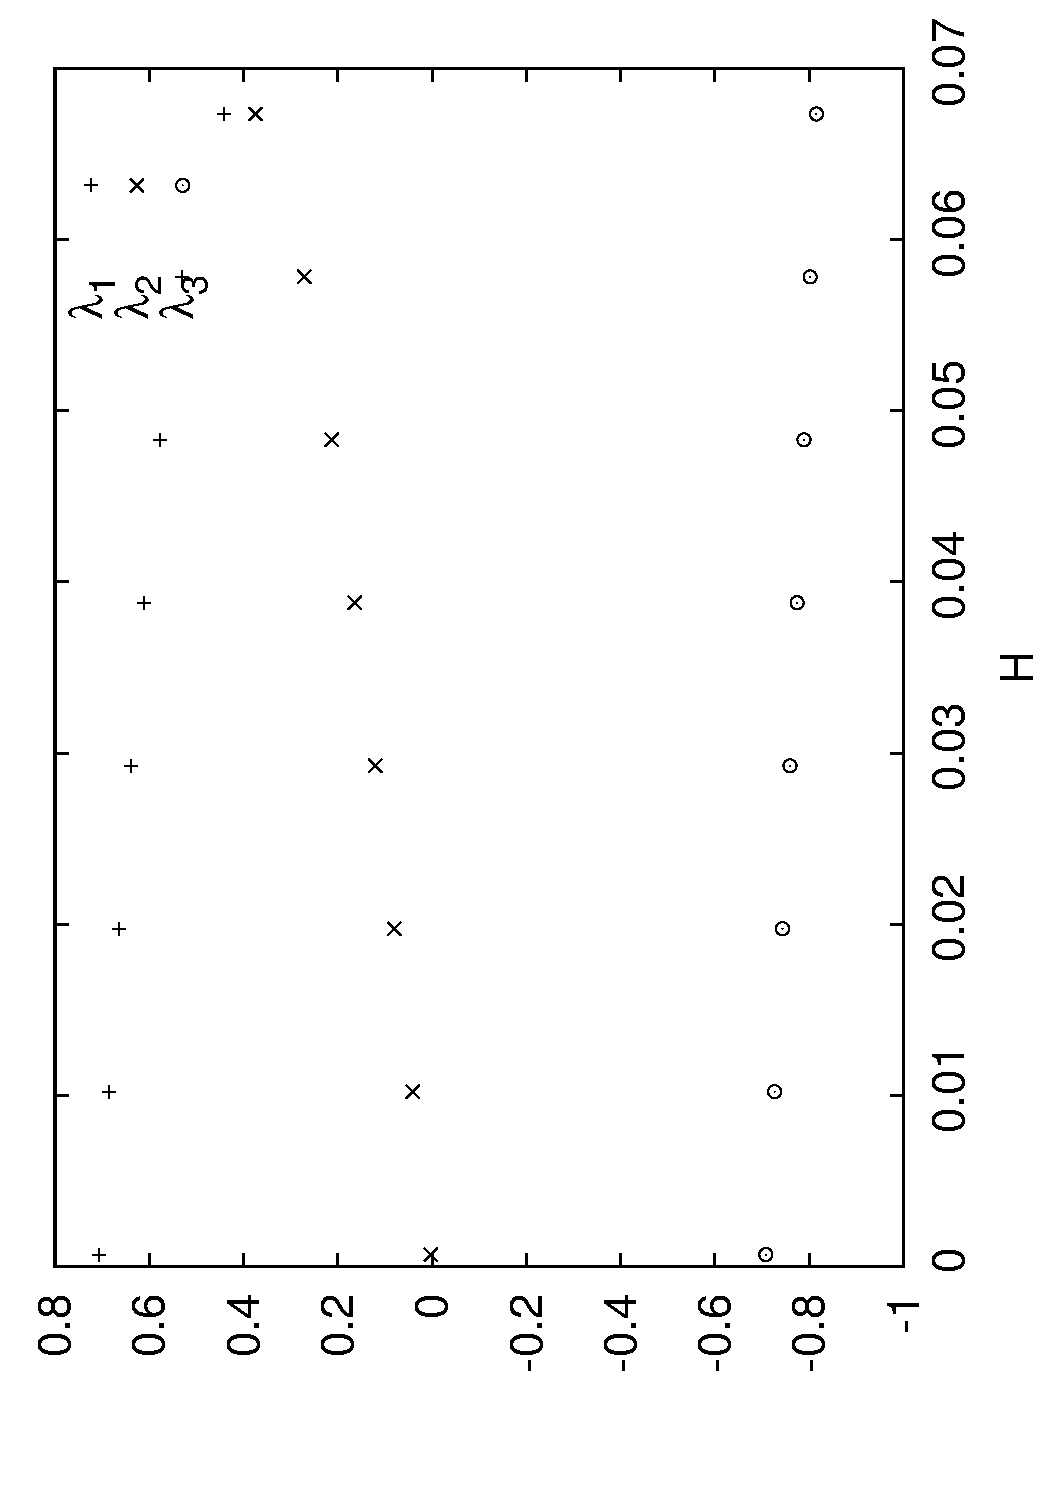
\includegraphics[angle=-90,width=\textwidth*7/8]{figures/lambdas}
\caption{Three roots shown for $I = 0.5$ and $0\le h \le H_c$. This figure is meant to help understand the limiting value of $\kappa$ which in turns helps in evaluating the gluing boundary condition}
\label{F:lambdas}
\end{center}
\end{figure}
Since the roots of $I u_1 - u_1^3 + 2 h$ for $h \le 0$ are the same as the roots of $I u_1 - u_1^3 - 2 h$ for $h \ge 0$, keeping the order $u_1^{2^+} > u_1^{2^-} > 0 > u_1^{2^*}$
\[
\begin{aligned}
\period_1(z)= \period_2(z) &= 2\int_{u_1^{{2}^{-}}}^{u_1^{{2}^{+}}}\frac{dt}{\sqrt{ t \,(I t - t^3 - 2 h)}}=2\, g K(\kappa)
\end{aligned}
\]
where
\[
g \equiv \frac{2}{\sqrt{\lambda_1 (\lambda_2-\lambda_3)}}, \qquad
\kappa^2 \equiv \frac{\lambda_3(\lambda_2 - \lambda_1)}{\lambda_1
(\lambda_2 - \lambda_3)} >0 ,\qquad \kappa^2 < \alpha^2 \equiv
\frac{\lambda_1 - \lambda_2}{\lambda_1} < 1
\]
By \citet[formula 256.12]{byrd54:_handb_of_ellip_integ_for}, the integrals
$\INT_{j}^1$,
% \[
% \begin{aligned}
%  \INT_1^1&\equiv\int_0^{\period_1}\frac{dt}{u_1(t)} = -
%
%
%  2\int_{u_1^{{1}^{-}}}^{u_1^{{1}^{+}}}\frac{d %u_1}{u_1^2\,\sqrt{f(u_1)}} \quad \text{for} \quad u_1 \le 0,\; h<0\\
%   \INT_2^1&\equiv\int_0^{\period_2}\frac{dt}{u_1(t)} =
%
%
%   2\int_{u_1^{{2}^{-}}}^{u_1^{{2}^{+}}}\frac{d %u_1}{u_1^2\,\sqrt{f(u_1)}} \quad \text{for} \quad u_1 \ge 0,\; h>0
%   \end{aligned}
% \]
reduce to
\begin{align*}
-\INT_1^1 = \INT_2^1 &= 2\int_{u_1^{2^-}}^{u_1^{2^+}} \frac{dt}{t \sqrt{t (I t - t^3 - 2 h)}}\\
&= 2 \int_{u_1^{2^-}}^{u_1^{2^+}} \frac{dt}{t \sqrt{t (u_1^{2^+}-t)(t-u_1^{2^-})(t-u_1^{2^*})}} = A_1 K(\kappa) + B_1 E(\kappa),
\end{align*}
where
\[
\begin{aligned}
 A_1&=2\,{\frac {g\left(\kappa-\alpha\right)\left
    (\kappa+\alpha\right)}{ \lambda_2{\kappa}^2}}= {\frac
  {4}{\lambda_3 \sqrt {\lambda_1 \left(\lambda_2 - \lambda_3
    \right)}\;}}\\
 B_1 &=2\,{\frac {g{\alpha}^2}{\lambda_2{\kappa}^2}}=
 \frac{4(\lambda_3 - \lambda_2)}{\lambda_2 \lambda_3 \sqrt
  {\lambda_1\left( \lambda_2-\lambda_3\right)}}
\end{aligned}
\]
Similarly, we can show the second set of integrals $\INT_{j}^2$
reduces to
\[
\begin{aligned}
 \INT_1^2 = \INT_2^2 &=
 2\int_{u_1^{{2}^{-}}}^{u_1^{{2}^{+}}}\frac{dt}{t^2\,\sqrt{ t \,(I t - t^3 - 2 h)}}\\
 &=2 \int_{u_1^{{2}^{-}}}^{u_1^{{2}^{+}}}\frac{dt}{t^2\,\sqrt{ t
   \, (u_1^{{2}^{+}}-t)(t-u_1^{{2}^{-}})(t-u_1^{{2}^{*}})}} =
 A_2\, K(\kappa) + B_2\, E(\kappa)
\end{aligned}
\]
where
\[
\begin{aligned}
 A_2&= \frac{2}{3}\,{\frac {g\left
    (3\,{\kappa}^4-6\,{\alpha}^2{\kappa}^2+2\,{
     \alpha}^4+{\alpha}^4{\kappa}^2\right
   )}{{\lambda_2}^2{\kappa}^4}}\\
 &= \frac{4}{3}\,{\frac {\left
    ({\lambda_3}^2+{\lambda_2}^2-2\,\lambda
    _3\lambda_2\right){\kappa}^2}{\sqrt
   {\lambda_1\left( \lambda_2-\lambda_3\right
    )}{\lambda_2}^2{\lambda_3}
   ^2}}+\frac{4}{3}\,{\frac
  {-{\lambda_3}^2+2\,\lambda_3\lambda_2
   +2\,{\lambda_2}^2}{\sqrt {\lambda_1\left
     (\lambda_2-
     \lambda_3\right)}{\lambda_2}^2{\lambda_3}^2}}\\
B_2 &=-\frac{4}{3}\,{\frac {g{\alpha}^2\left(-3\,{\kappa}^2+{\alpha}^2+{
\alpha}^2{\kappa}^2\right)}{{\lambda_2}^2{\kappa}^{4}}}\\
& = -\frac{8}{3} {\frac{\left(\lambda_2-\lambda_3\right)^2{\kappa}^{2}}{\sqrt{\lambda_1\left(\lambda_2-\lambda_3\right)}{\lambda_2}^2{\lambda_3}^2}}-\frac{8}{3}\,{\frac{\left(\lambda_2-\lambda_3\right)\left(\lambda_2+2\,\lambda_3\right)}{\sqrt{\lambda_1\left(\lambda_2-\lambda_3\right)}{\lambda_2}^2{\lambda_3}^2}}
\end{aligned}
\]

The drift and diffusion terms are evaluated making use of these
results.

\section{Simplification of the Gluing Condition}
\label{A:gluing BC simplification}

The general form for the conservation of probability flux condition was given in equation~\eqref{E:cpfc}. The probability flux, $J$, is given in equation~\eqref{E:prob flux} and $\nu^n$ represents the outward normal vector of leaf $n$. $z = (h,i) = \mathcal{O}$ is used to denote the gluing vertex. In this appendix we show that the conservation of probability flux condition simplifies to equation~\eqref{E:cpfc simplified}.

The first step towards this simplification is to exploit the fact the gluing vertex is aligned with the $h=0$ axis, therefore equation~\eqref{E:cpfc} for the two-leaf autoparametric system becomes
\begin{equation}
\lim_{h \to 0} \left(J^1_1(h,i) - J^2_1(h,i)\right) = 0.
\label{E:cpfc intermediate}
\end{equation}
Next, individual terms of the probability flux must be considered. First we consider those simplifications that can be made analytically. From~\eqref{E:drift h}, it follows that $\mathring{\mathfrak{b}}_1^n = - (\zeta_o + 2\zeta_p) H \period_n$ (for $n=1,2$.) Since as $h \to 0$, the period is asymptotically equivalent to $\period(z) \sim \ln |H|$, the following results:
\[
\lim_{h \to 0} \mathring{\mathfrak{b}}_1^n = 0
\]
Similarly, from equation~\eqref{E:diffusion hi} it follows that $\mathring{\Aa}_{12}^n = \sigma^2 S_{\xi\xi}(1) H \period_n$. Again, the asymptotic behavior of $\period(z)$ yields:
\[
\lim_{h \to 0} \mathring{\mathfrak{a}}_{12}^n = 0
\]
The fact that $\mathring{\mathfrak{a}}_{11}^1 = \mathring{\mathfrak{a}}_{11}^1 = \sigma^2 S_{\xi\xi}(1) I \sqrt{I}/3$ (see equation~\eqref{E:lim drift_11}) is also used to simplify equation~\eqref{E:cpfc intermediate}.

The final two simplifications are
\begin{align*}
\lim_{h \to 0} \frac{\partial \mathring{\Aa}_{11}^n}{\partial h} &= 0,&
\lim_{h \to 0} \frac{\partial \mathring{\Aa}_{12}^n}{\partial i} &= 0
\end{align*}
for $n=1,2$. These two simplifications can be demonstrated numerically, as shown in Figures~\ref{F:lim a11} \& \ref{F:lim a12}.

\begin{figure}
\begin{center}
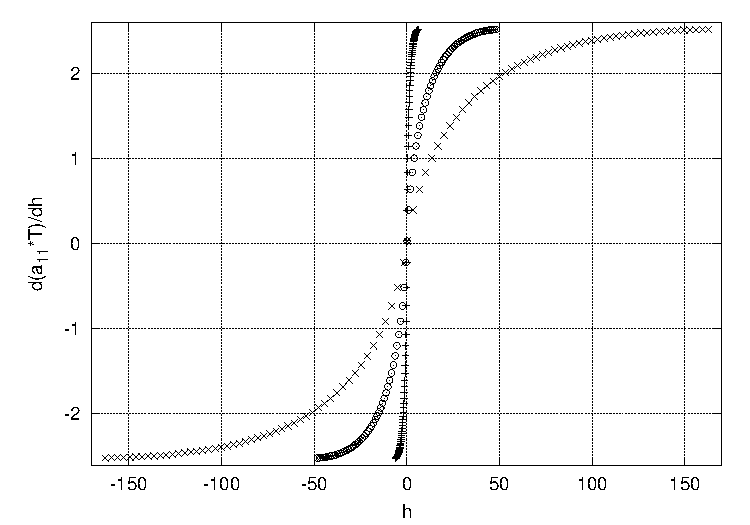
\includegraphics[width=\textwidth*7/8,angle=0]{figures/lim_a11}
\caption{Numerical demonstration that $\lim_{h \to 0} \frac{\partial\mathring{\Aa}_{11}^n}{\partial h} = 0$. Each dataset is for a different value of $i$.}
\label{F:lim a11}
\end{center}
\end{figure}

\begin{figure}
\begin{center}
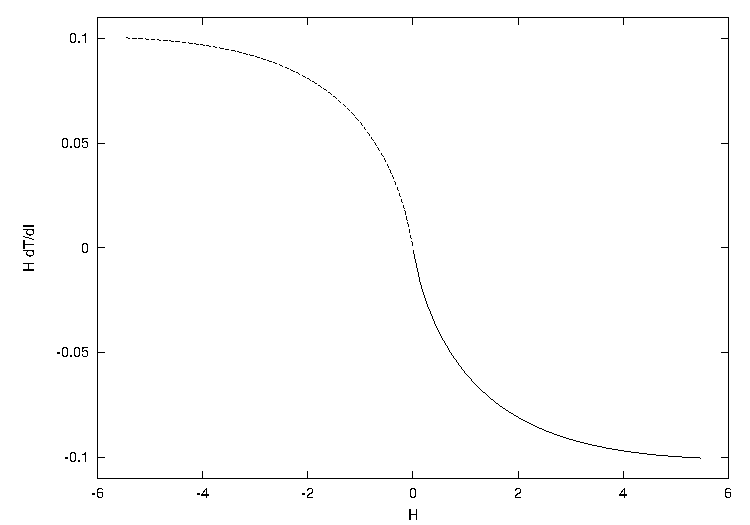
\includegraphics[width=\textwidth*7/8]{figures/cpfbc_numerical_demo}
\caption{Numerical demonstration that $\lim_{h \to 0} h \cdot d\period/di = 0$. This result demonstrates that $\partial \mathring{\Aa}_{12}/\partial I = 0$, that is used to simplify the conservation of probability flux condition.}
\label{F:lim a12}
\end{center}
\end{figure}

% Kludge to fix Figure numbering problem
\begin{figure}
\begin{center}
\label{F:lim a122}
\end{center}
\end{figure}

%% How might numerical simplifications be made analytic?


\backmatter

\bibliographystyle{abbrvnat}
\bibliography{main}

\aubio
% -*- mode: LaTeX -*-

Kristjan Onu received a bachelor's degree in applied mathematics from the University of Western Ontario, Canada, in 2001. In 2003, he completed a master's of science in theoretical and applied mechanics from the University of Illinois at Urbana--Champaign. His doctoral research has allowed him to study stochastic dynamical systems, averaging methods and scientific computing.


\end{document}
